\documentclass[
12pt, % The default document font size, options: 10pt, 11pt, 12pt
%oneside, % Two side (alternating margins) for binding by default, uncomment to switch to one side
english, % ngerman for German
singlespacing, % Single line spacing, alternatives: onehalfspacing or doublespacing
%draft, % Uncomment to enable draft mode (no pictures, no links, overfull hboxes indicated)
%nolistspacing, % If the document is onehalfspacing or doublespacing, uncomment this to set spacing in lists to single
%liststotoc, % Uncomment to add the list of figures/tables/etc to the table of contents
%toctotoc, % Uncomment to add the main table of contents to the table of contents
%parskip, % Uncomment to add space between paragraphs
%nohyperref, % Uncomment to not load the hyperref package
headsepline, % Uncomment to get a line under the header
%chapterinoneline, % Uncomment to place the chapter title next to the number on one line
%consistentlayout, % Uncomment to change the layout of the declaration, abstract and acknowledgements pages to match the default layout
]{mormontThesis} % The class file specifying the document structure

\usepackage[utf8]{inputenc} % Required for inputting international characters
\usepackage{csquotes}
\usepackage[T1]{fontenc} % Output font encoding for international characters

\usepackage{mathpazo} % Use the Palatino font by default

\usepackage[backend=biber, style=ext-authoryear, maxnames=2, maxbibnames=4, natbib=true]{biblatex} 

\addbibresource{thesis.bib} % The filename of the bibliography

% for having brackets when citing
\DeclareOuterCiteDelims{parencite}{\bibopenbracket}{\bibclosebracket}

\DeclareFieldFormat{citehyperref}{%
  \DeclareFieldAlias{bibhyperref}{noformat}% Avoid nested links
  \bibhyperref{#1}}

\DeclareFieldFormat{textcitehyperref}{%
  \DeclareFieldAlias{bibhyperref}{noformat}% Avoid nested links
  \bibhyperref{%
    #1%
    \ifbool{cbx:parens}
      {\bibcloseparen\global\boolfalse{cbx:parens}}
      {}}}

\savebibmacro{cite}
\savebibmacro{textcite}

\renewbibmacro*{cite}{%
  \printtext[citehyperref]{%
    \restorebibmacro{cite}%
    \usebibmacro{cite}}}

\renewbibmacro*{textcite}{%
  \ifboolexpr{
    ( not test {\iffieldundef{prenote}} and
      test {\ifnumequal{\value{citecount}}{1}} )
    or
    ( not test {\iffieldundef{postnote}} and
      test {\ifnumequal{\value{citecount}}{\value{citetotal}}} )
  }
    {\DeclareFieldAlias{textcitehyperref}{noformat}}
    {}%
  \printtext[textcitehyperref]{%
    \restorebibmacro{textcite}%
    \usebibmacro{textcite}}}

\usepackage{lipsum}

% ========== %
%  Acronyms  %
% ========== %
\makeglossaries

\newacronym{acc}{ACC}{accuracy}
\newacronym{ai}{AI}{artificial intelligence}
\newacronym{afds}{AFDS}{attentive feature distillation and selection}
\newacronym{auc}{AUC}{area under the curve}
\newacronym{bce}{BCE}{binary cross-entropy}
\newacronym{bn}{BN}{batch normalization}
\newacronym{cnn}{CNN}{convolutional neural network}
\newacronym{ct}{CT}{computed tomography}
\newacronym{cv}{CV}{cross-validation}
\newacronym{dl}{DL}{deep learning}
\newacronym{dp}{DP}{digital pathology}
\newacronym{erm}{ERM}{empirical risk minimization}
\newacronym{etdic}{ET-DIC}{extremely randomized trees as direct-learner}
\newacronym{etfl}{ET-FL}{extremely randomized trees as feature-learner}
\newacronym{et}{ET}{extremely randomized trees}
\newacronym{fpr}{FPR}{false positive rate}
\newacronym{fcn}{FCN}{fully-convolutional network}
\newacronym{fc}{FC}{fully connected}
\newacronym{fnab}{FNAB}{fine-needle aspiration biopsy}
\newacronym{gan}{GAN}{generative adversarial networks}
\newacronym{heeo}{H\&E}{hematoxylin \& eosin}
\newacronym{ilsvrc}{ILSVRC}{ImageNet Large Scale Visual Recognition Challenge}
\newacronym{loto}{LOTO}{leave-one-task-out}
\newacronym{ml}{ML}{machine learning}
\newacronym{mlp}{MLP}{multi-layer perceptron}
\newacronym{mtl}{MTL}{multi-task learning}
\newacronym{nlp}{NLP}{natural language processing}
\newacronym{ovo}{OVO}{one-vs-one}
\newacronym{ovr}{OVR}{one-vs-rest}
\newacronym{relu}{ReLU}{rectified linear unit}
\newacronym{rfe}{RFE}{recursive feature elimination}
\newacronym{roc}{ROC}{receiver operating characteristic}
\newacronym{sgd}{SGD}{stochastic gradient descent}
\newacronym{sl}{SL}{supervised learning}
\newacronym{ssl}{SSL}{semi-supervised learning}
\newacronym{svm}{SVM}{support-vector machine}
\newacronym{tl}{TL}{transfer learning}
\newacronym{tpr}{TPR}{true positive rate}
\newacronym{usl}{USL}{unsupervised learning}
\newacronym{vgg}{VGG}{very deep convolutional neural network}
\newacronym{vit}{ViT}{vision transformer}
\newacronym{wsi}{WSI}{whole-slide image}
\newacronym{wsl}{WSL}{weakly-supervised learning}
\renewcommand{\glsnamefont}[1]{\textsc{\bfseries #1}}
\newcommand{\acrfirst}[1]{\acrlong{#1} (\acrshort{#1})}
\newcommand{\acrfirstbf}[1]{\textbf{\acrlong{#1}} (\acrshort{#1})}
\newcommand{\acrfirstit}[1]{\textit{\acrlong{#1}} (\acrshort{#1})}

% ================= %
%  Custom commands  %
% ================= %
\newcommand{\ie}{\textit{i.e.~}}
\newcommand{\eg}{\textit{e.g.~}}
\newcommand{\etal}{\textit{et al.~}}
\newcommand{\aka}{\textit{a.k.a.~}}
\newcommand{\resp}{\textit{resp.~}}
\newcommand{\etc}{\textit{etc}}
\newcommand{\vs}{\textit{vs.}}
\newcommand{\quoteit}[1]{``\textit{#1}"}
\newcommand{\TODO}[1]{{\color{red}(TODO: #1)}}
\newcommand{\argmax}[1]{\text{arg}\,\underset{#1}{\text{max}}\,}
\newcommand{\argmin}[1]{\text{arg}\,\underset{#1}{\text{min}}\,}
\newcommand{\rocauc}{\acrshort{roc} \acrshort{auc}}
\newcommand{\rocaucs}{\rocauc~}
\newcommand{\vect}[1]{\mathbf{#1}}

\author{Romain Mormont}
\title{Addressing data scarcity with deep transfer learning and self-training in digital pathology}

\begin{document}% 
\pagestyle{empty}

\makeatletter

\newgeometry{left=1in,top=1in,bottom=1in}

\begin{titlepage}

  \begin{center}
    {\Large University of Liège} \\
    \vspace{10pt}
    Faculty of Applied Sciences \\
    Department of Electrical Engineering \& Computer Science

    \vfill 

    PhD dissertation 

    \vspace{2em}

    {
      \color{primary}
      \rm
      \bf
      \Huge
      \@title
    }

    \vspace{1em}

    by \@author

    \vfill


    \begin{minipage}{0.4\linewidth}
      
\includegraphics[scale=0.22]{uliege_logo_rvb_pos.png}
    \end{minipage}
    \begin{minipage}{0.55\linewidth}
      \begin{flushright}
        Advisors: Pierre Geurts \& Raphaël Marée \\
        September 2022
      \end{flushright}
    \end{minipage}

  \end{center}
\end{titlepage}

\restoregeometry 

\makeatother


% =========== %
% FRONTMATTER %
% =========== %
\frontmatter


\chapter*{Jury}
\chapter*{Acknowledgements}

Un doctorat est une aventure parsemée de joies, de peines et d'obstacles. Cette aventure, je n'en aurais jamais vu le bout sans bon nombre de personnes que j'aimerais remercier. 

\vspace{15pt}

Mes premiers remerciements vont évidemment à mes promoteurs, Pierre et Raphaël. Lorsqu'en 2015, j'ai contacté Pierre à la recherche d'un sujet de TFE en ``machine learning sur des images'' et qu'il m'a mis en contact avec Raphaël, je n'aurais jamais osé m'imaginer que cela m'amènerait environ 7 ans plus tard à défendre une thèse de doctorat. Je me souviens encore très bien de la première réunion avec Raphaël à l'extérieur de Montefiore et l'introduction à Cytomine puis les réunions de suivi avec le duo au GIGA. Ces premiers échanges furent aussi enrichissants qu'agréables.

Je me souviens également de la discussion avec Pierre au cours de laquelle il m'a proposé d'entamer une thèse. Si le challenge avait attisé ma curiosité, ce sont aussi les qualités humaines de mes futurs promoteurs qui m'ont convaincues d'accepter la proposition. On entend souvent parler de doctorats qui tournent mal à cause d'une relation doctorant-promoteur compliquée, voire toxique. Dans mon cas, ce fut tout le contraire. J'ai eu l'infinie chance de tomber sur deux personnes bienveillantes, encourageantes, curieuses de ce que j'avais à proposer, toujours prêtes à accorder du temps pour une réunion ou une discussion. Au-delà des aspects humains, leur apport scientifique, technique et leur complémentarité dans ces deux domaines abordés dans ma thèse m'ont évidemment grandement aidé et m'ont permis d'apprendre énormément. Pierre, Raphaël, je ne vous remercierai probablement jamais assez d'avoir cru en moi et de m'avoir permis d'arriver où je suis maintenant!

\vspace{15pt}

J'aimerais aussi remercier tous les collègues que j'ai eu la chance de côtoyer au long de ces six années. Que ça soit en temps de midi, en LAB Meeting, en conférence ou autres, votre présence et nos discussions étaient toujours bien agréables. Vous avez contribué à me faire aimer mon travail ! Un grand merci à Laurine, Jean-Michel, Ulysse, Vân Anh, Pierre, Raphaël, Michaël, Antho, Navdeep, Marie, Antoine, Pascal L., Matthia, Nicolas, Rémy, Pascal F., et encore plein d'autres que j'oublie fort probablement (désolé!).

\vspace{15pt}

Je souhaite également remercier les membres du jury internes, Louis et Marc, et externes, Christine Decaestecker et Francesco Ciompi, qui ont pris le temps de lire mon travail en détail et m'ont fourni un feedback précieux. Merci également à Laurine, Fabrice, Michel, Ulysse et Jean-Michel qui ont relu ce manuscrit avant soumission.

\vspace{15pt}

Ce travail n'aurait jamais été possible sans l'accès à des ressources de calcul et j'aimerais également remercier toutes les personnes m'ont permis de près ou de loin d'y avoir accès. Remerciements, donc, à tous les professeurs et équipes de Montefiore qui ont financé le cluster GPU et remerciements particuliers à Joeri qui a mis en place l'infrastructure.  

\vspace{15pt} 

Amis et famille, je ne vous oublie pas ! Durant ces six années remplies de hauts et de bas, au fond de moi, je n'ai jamais perdu cette petite flamme alimentée par votre amour, amitié et soutien. Quoiqu'il se passe, quelle que soit l'épreuve, je sais que je peux compter sur vous et mine de rien, ça fait toute la différence. 

À ma famille, Papa, Maman et Odile en tête mais aussi tous les autres, merci pour votre présence et votre soutien inconditionnel. Un remerciement tout particulier à Babone et Papy Linlin de m'avoir accueilli tous les vendredis pendant presque un an. Chez vous, j'ai trouvé un havre de quiétude et de concentration qui m'ont permis d'avancer significativement dans la rédaction de ce manuscrit. Un grand merci à toi aussi Florence, qui m'a rejoint sur la fin du parcours pour ton soutien et ton amour pendant la finalisation du travail. 

Les amis, ensuite, que vous soyez présent physiquement ou derrière un écran et un micro, vous m'avez aidé plus que vous ne le pensez dans les périodes difficiles (pandémie, je te vois). Les Componions évidemment (Fabrice, Chloé, Élo, Arnaud, Laurine, Quentin, Hubert), merci pour votre présence, merci d'être ce que vous êtes et de ce que nous devenons. Floriane, merci pour tes visites lors de passages à Montefiore et nos discussions techniques ou non. Michel, merci de m'avoir fait visiter le service d'anatomopathologie du CHU de Liège. Sans toi, mon chapitre 3 ne serait pas ce qu'il est. Les colocs en commençant par Charly, Mirabelle et Nicolas. Que ce fut enrichissant d'emménager et de vivre ensemble. Je n'oublie pas ceux qui ont suivi aussi: Hubert, Michaël, Jérôme, Jiyeon. L'amitié n'est pas toujours là où on l'attend et peut parfois se développer par écran interposé: je tiens à vous remercier les Bloude et en particulier la team "Off" pour tous les bons moments passés ensemble en ligne qui m'ont grandement aidé à passer le cap de la pandémie.

\vspace{15pt}

J'aimerais clôturer ces remerciements avec une mention toute particulière pour toi, Nonno, qui nous a quittés voilà maintenant 11 ans. Tu avais 25 ans et ne savais ni lire ni écrire quand tu as quitté ton Italie natale pour trouver un travail afin de demander la main de Nonna. Tu as échangé le soleil et la chaleur des Pouilles pour le ciel gris belge, la pénombre et la poussière des mines. Ce sont les combats que vous avez menés avec Nonna pour permettre à vos enfants de vivre une vie décente qui m'ont permis d'obtenir le titre de Docteur aujourd'hui. C'est pour cela que je te dédie cette réussite. 


\chapter*{Contents}
\tableofcontents


% ========== %
% MAINMATTER %
% ========== %
\mainmatter
\pagestyle{scrheadings}

% CHAPTERS
\chapter{Introduction}

\section{Context}

Artificial intelligence (\acrshort{ai}) and, more specifically, \acrfirstit{ml} has been through quite a journey since its inception in the 1940s and 1950s. From a small research domain, it has grown into a massive rapidly-developing field of research and applications with ramifications in many branches of science and technology. This growth is not surprising in a world where computers become more and more powerful and data, the bread-and-butter of machine learning, is becoming increasingly collectable, structured, available and queryable. Applications of \acrlong{ml} are as varied as they are numerous: spam filtering, fraud detection, face recognition, self-driving cars, robotics and automation, medical data analysis and diagnosis, simulation in particle physics... to name only a few. While it has already revolutionized many domains, \acrlong{ml} research has still a bright future ahead. In the last decade only, along with \acrfirstit{dl}, several new family of techniques have been (re-)discovered and have enabled unexpectedly-fast progress (\eg \acrlong{cnn}, \acrlong{gan}, transformers). One can only expect that the next ground-breaking \acrshort{ml} method is on the brink of being discovered in a research lab somewhere around the world. Aside from that, research is still ongoing of many fronts such as understanding, applying or improving existing methods.

Medicine is among the numerous fields where \acrlong{ml} is showing great promises. Although often misrepresented in the mainstream media as a tool that will eventually replace practitioners, the real potential of \acrlong{ml} in medicine actually lies in its capacity to become a strong, resilient and consistent assistant to the physicians \parencite{rajkomar2019machine}, assisting them for tasks ranging from diagnosis and analysis to paperwork. Rather than replacing physicians, an \acrshort{ai}-based diagnosis system would be able to complement their opinion and advise them based on experiences of millions of other patients and colleagues. Moreover, such a system would be able to produce these advice based on a very large number of parameters and sources of data that a human could not realistically consider (imaging, written reports, laboratory values, vital signs). However, the road to an \acrshort{ai}-assistant is still long and many questions and challenges have yet to be addressed. From a scientific standpoint, current research mostly focuses on improving solutions for tasks of significantly smaller scale and scope (\eg outlining organs in x-rays, detecting disease in \acrshort{ct}-scans, classifying skin cancer as malignant or benign \TODO{non imaging example}). Many recent contributions, although some arguably lacking scientific rigor, have claimed to have matched or surpassed human experts accuracies by applying machine and \acrlong{dl} methods on different medical tasks \parencite{nagendran2020artificial}. Whereas progress is certain, many challenges have yet to be solved. 

One of these major challenges is \textit{data scarcity}. Not that data itself is lacking as \parencite{pramanik2019healthcare} reported that the amount of health data stored worldwide could reach 2,258 exabytes in 2020. What is scarce is actually data that is at least partially annotated and of good-enough quality to be used to train \acrlong{ml} models. Data scarcity has many causes: privacy concerns prevent sharing patient data, the annotation process is time-consuming and expensive... The usage of \acrlong{dl} makes it even worse as \acrshort{dl} methods are very data-hungry.

In this thesis, we are interested in one specific field of medicine and, more specifically, medical imaging: \acrfirstit{dp}. Microscope have been used in medicine to analyse samples (\eg cells, tissue or blood) since the 17th century \parencite{hajdu2002first} but recent technological progress has enabled the digitization of microscope glass slides into images called \textbf{\acrlong{wsi}s} (\acrshort{wsi}). Digital pathology concerns all the aspects of acquiring, managing, sharing and interpreting these \acrshort{wsi}s \parencite{doolan2019whatisdp}. With the help of image management systems and new visualization tools, \acrshort{wsi}s have greatly facilitated the day-to-day work of practitioners (\eg pathologists, biologists) who do not have to manipulate physical glass slides anymore. More importantly, the digitization has opened the way for \textit{automated analysis} with computer vision techniques, including \acrlong{ml} \parencite{ciompi2021editorial}. Whereas acquiring and managing \acrshort{wsi}s provide interesting challenges, our contributions focus mostly on (automated) analysis and, throughout the thesis, we will refer to this part when using the term \quoteit{\acrlong{dp}}.

\begin{figure}
  \centering
  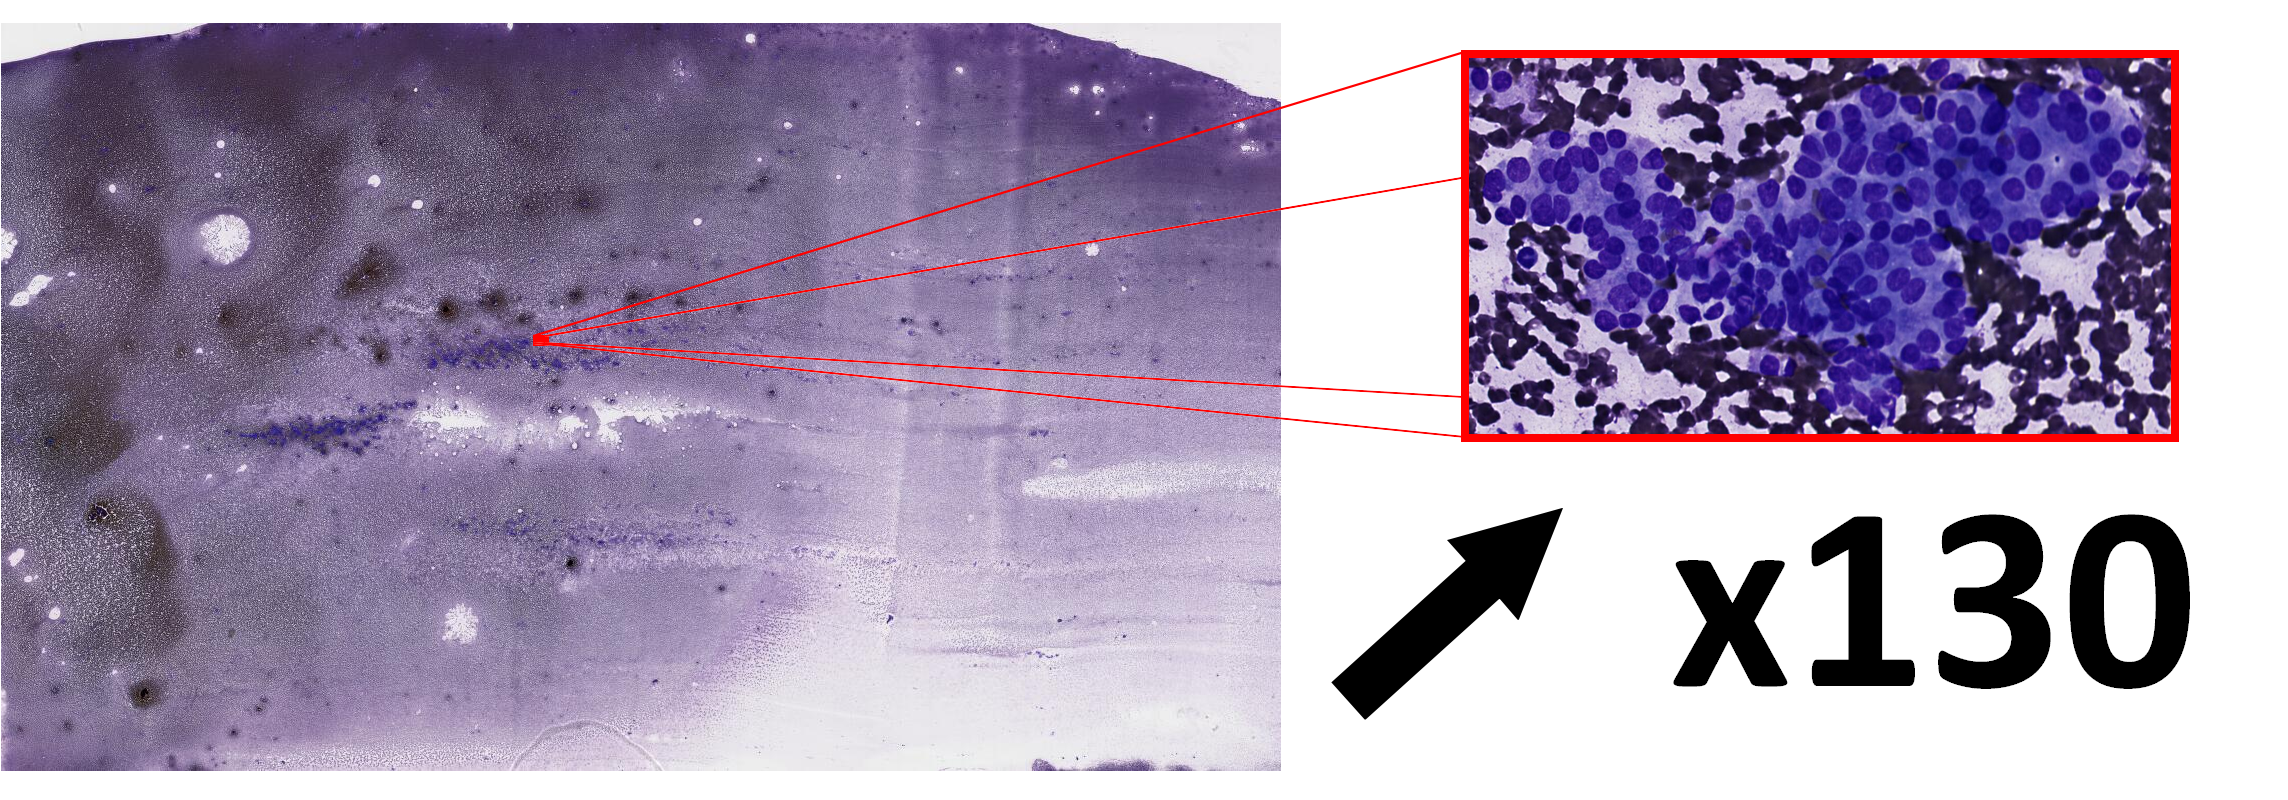
\includegraphics[scale=0.25]{intro/whole-slide-dim.png}
  \caption{A typical \acrlong{wsi} of size 163840 $\times$ 95744 pixels and file size of 2.3 gigabytes. To the left is the original slide and to the right is a structure of interest at zoom level $\times130$ (size in pixels: 1354 $\times$ 736)}.
  \label{fig:intro:wsi}
\end{figure}

Automating the analysis of \acrshort{wsi}s is quite a challenge. Typically, a \acrshort{wsi} is a very large image that can reach few billion pixels at minimum zoom level (see Figure \ref{fig:intro:wsi}, a single file can weight several gigabytes) therefore making classical computer vision methods inapplicable without adaptation. The image content is usually complex (see Figure \TODO{find mosaic}) which excludes the use of simplistic computer vision methods (\eg thresholding). This explains why \acrlong{dl} is currently so popular among \acrlong{dp} researchers because of its ability to cope with complexity. However, the use of \acrlong{dl} is hampered by data scarcity of which the field is not spared since billion-pixels images are as tedious to analyse as to annotate exhaustively, even for trained pathologists. The data scarcity problem is made worse by the variability introduced by the process of \quoteit{transforming} a sample into a slide and then into a digital image.


\section{Contributions}

In this thesis, we explore different ways of tackling data scarcity in \acrlong{dp} using \acrlong{dl}. Our contributions leverage \acrfirst{tl}, \acrfirst{mtl} and self-training which we apply to the tasks of image classification and segmentation. \TODO{elaborate}

Our contributions are as follows.

First, we review, compare and study different deep \acrlong{tl} techniques using 8 classification datasets in order to evaluate the viability and best practices of \acrlong{tl} in \acrlong{dp}. We show that using neural networks pre-trained on a dataset unrelated to digital pathology (\ie ImageNet) is indeed interesting compared to training a network from scratch. We also draw guidelines from our experiments on how the transfer should be performed.

We then propose a \acrlong{mtl} architecture and training scheme for pre-training a network based on an ensemble of potentially-small datasets rather than a single large dataset. We use these in order to pre-train a neural network on 22 classification \acrlong{dp} datasets and show that our resulting models yield competitive results compared to networks pre-trained on ImageNet. The code and models are also publicly available online. \TODO{url}

The third contribution concerns image segmentation in an imperfect annotation setting. More precisely, we investigate a self-training scheme for training a U-Net architecture on a \acrshort{dp} dataset where a pathologist only annotated the images partially.

\TODO{final contribution}


\section{Outline}

The thesis is structured in four parts. 

Part \ref{part:background} introduces \acrlong{ml} and \acrlong{dp}. It is not intended to explain the matters in depth but rather to give sufficient background for a reader with a basic knowledge of machine learning to understand the contributions.

Chapter \ref{chap:backml} focuses on machine learning and presents \TODO{complete}... 

Chapter \ref{chap:backdp} focuses on digital pathology and presents \TODO{complete}...

Part \ref{part:transfer} presents our first and second contributions which are both related to \acrlong{tl}. 

Chapter \ref{chap:comp} ...

Chapter \ref{chap:mtask} ...

Part \ref{part:segmentation} presents our third contribution on self-training in an imperfect dataset setting. 

Chapter \ref{chap:strain}, presents ...

Part \ref{part:software} presents our software contributions including Biaflows and SLDC.

\section{Publications}

\begin{itemize}
  \item \fullcite{mormont2016sldc}
  \item \fullcite{mormont2018comparison}
  \item \fullcite{mormont2020multi}
  \item \fullcite{rubens2020biaflows}
\end{itemize}



\part{Background}
\chapter{Machine learning}
\label{chap:backml}

\begin{overview}{Overview}
The goal of this chapter is to provide machine learning background and keys to understand our contributions. It is not aimed at being an exhaustive tour of the field of machine learning but rather an overview of topics relevant to this thesis. For the readers who would still like to deepen their knowledge about these methods, we provide pointers to relevant litterature. In this chapter, we also introduce the notations that we use throughout this thesis.

Section \ref{sec:backml:whatisml} provides a short definition of \acrlong{ml} and a first example of an \acrshort{ml} problem. Section \ref{sec:backml:families} explores the different ways the field of \acrlong{ml} can be structured (\eg supervised vs. unsupervised learning, classification vs. regression, classical machine vs. \acrlong{dl}...) in order to position our work in its context. Section \ref{sec:backml:modeleval} discusses what guides \acrlong{ml} model training from a theoritical point of view. Then, it presents practical concerns regarding model selection and evaluation. It finally provides a description of different evaluation metrics used in this thesis. This chapter then shifts its focus on specific machine learning methods and algorithms: \acrlong{svm} in Section \ref{sec:backml:svm}, tree-based methods in \ref{sec:backml:treebased} and deep learning in Section \ref{sec:backml:deeplearning} in which we also discuss more thouroughly deep transfer learning (see Section \ref{ssec:backml:dl:deeptransfer}). In the final Section \ref{sec:backml:wrapup}, we wrap up by positioning our work in the context of \acrlong{ml}.
\end{overview}

\section{What is machine learning ?}
\label{sec:backml:whatisml}

A computer program is said to learn from experience $E$ with respect to some class
of tasks $T$ and performance measure $P$ if its performance at tasks in $T$, as
measured by $P$, improves with experience $E$ \parencite{mitchell1997machine}.
Machine learning concerns the study of such programs, commonly referred to as
\textit{models}, and how to build them by learning. A \textit{model} $h$ can be
seen a function taking an input $\vect{x} \in \mathcal{X}$ (\aka observation,
example, instance) and producing an ouput $h(\vect{x})$ or $\hat{y} \in \mathcal{Y}$.
Entities $\vect{x}$ and $h(\vect{x})$ are n-dimensional tensors and can encode
many kind of data types: data record, image, graph, time series, text... When
$\vect{x}$ is a vector, its components are commonly called \textit{features},
\textit{variables} or \textit{attributes}. A model can have several inputs (\resp
outputs) in which case $\vect{x}$ (\resp $y$) is a $n$-tuple.

In \acrlong{ml}, a model is built by a \textit{learning algorithm}. Formally, a
learning algorithm is defined by a set $\mathcal{H}$ of candidate models called
the \textit{hypothesis space}, a performance measure $P$ for a model and an
optimization strategy. As input, the algorithm is provided with \textit{training data}
(the experience $E$, \aka learning or training set) that it uses to build and
optimize the model. The algorithm output is a model $h \in \mathcal{H}$ that
maximises the performance criterion. A model being built by a learning algorithm
is said to be in the \textit{training phase}. When this model has been trained
and is used on new data, it is said to be in the \textit{inference phase}.

As an example, a common task is \textit{natural image classification} where the
model must assign a label to a picture. For instance, one would want to detect
whether a picture contains a human, an animal or an inanimate object. In this
case, considering that the images are encoded with integers, the input space is
the set of all possible color images: $\mathcal{X} \subset \mathbb{N}^{r\times c\times b}$
where $r$, $c$ and $b$ are respectively the image width, height and number of
channels (which equals to 3 in the case of RGB color images). The output space is
composed of the 3 labels of interest: $\mathcal{Y} = \left\{\textit{human}, \textit{animal}, \textit{object}\right\}$.
The model would take an image $\vect{x} \in \mathcal{X}$ as input and, based on
its content, output $\hat{y}$, one of the predefined labels. This label $\hat{y}$
might be false if the model makes a mistake. Therefore, for the sake of distinction,
the correct label is denoted $y$ (\aka ground truth). As a performance measure
$P$, one could assess the correctness of the ouput label by assigning 0 to correct
predictions and 1 to errors. This performance measure is called the \textit{zero-one loss}
and is written as:

\begin{equation}
\ell_{0-1}(y, \hat{y}) = \mathbb{1}_{y\neq\hat{y}}
\end{equation}

There are numerous tasks beyond natural image classification to which \acrlong{ml}
can be applied nowadays. In the next sections, we will discuss some of them and
dive a little deeper into algorithms and topics related to learning which are
relevant to this thesis.

\section{Families of learning methods}
\label{sec:backml:families}

There are many ways to structure the ecosystem of \acrlong{ml} methods. This
section explores some of them.

\subsection{Supervised learning}
\label{ssec:backml:sl}

\textit{Supervised learning} (\acrshort{sl}) regroups methods where the learning
process is guided by an output signal. We formalize a supervised task as the tuple
$\left(\mathcal{X}; \mathcal{Y}; p(\vect{x}, y)\right)$ where $\mathcal{X}$ and
$\mathcal{Y}$ are respectively the input and output spaces and $p(\vect{x}, y)$
is a probability distribution over those joint spaces. The learning algorithm is
provided with a training set
\begin{equation}
\label{eqn:backml:supervised}
\mathcal{S} = \left\{(\vect{x}_i, y_i) \mid i = 1,...,n ; (\vect{x}_i, y_i) \sim p(\vect{x}, y) \right\}
\end{equation}
where $y_i \in \mathcal{Y}$ is the output signal for the observation
$\vect{x}_i \in \mathcal{X}$. The learning algorithm objective is to find a model
$h \in \mathcal{H}$ that approximates at best the output.

When the output space is a finite set of discrete values
$\mathcal{Y} = \left\{v_1, v_2, ..., v_C\right\}$, the problem is called
\textit{classification}. The $v_i$ elements are called the classes (or label) and
$C$ denotes the cardinality of the set $\mathcal{Y}$ (\ie the number of classes).
When $C = 2$, the problem is said to be \textit{binary}. In classification, the
model should predict the most probable output class given an example:
\begin{equation}
\hat{y}_i = \argmax{y_k \in \mathcal{Y}} p(y=y_k|\vect{x}=\vect{x}_i)
\end{equation}
Examples of classification tasks are for instance assigning a label to an image
or detecting whether an email is a spam or not.

When the output space is continuous and the output is a real scalar value, the
problem is called \textit{regression}. In this case, the model should predict the
expected value $y$ given any input $\vect{x}_i$:
\begin{equation}
h(\vect{x}_i) = \mathbb{E}\left[y|\vect{x}=\vect{x}_i\right]
\end{equation}
Examples of regression problems are trying to predict the price of a house given
its area, the amount of product generated by a factory in a given time period or
the review score of a product on an e-commerce platform.

Some models can also predict structured outputs. This is the case with
\textit{image segmentation} which focuses on classifying each pixel of an image
(\ie answering the question: what kind of object does this pixel belong to in the
image?). The output of the model is a segmentation mask where pixel at row $i$
and column $j$ of the image is classified as $\hat{y}_{ij} \in \mathcal{Y}$. For
some tasks, a mask is not always necessary, one is rather interested in the coarse
location of the objects. This kind of task is called \textit{detection} for which
the output of the model, the location, can be encoded as image coordinates $(i, j)$
representing the object's center of gravity or any of its points. Another common
representation is the bounding box, a box containing exactly the object of interest,
encoded by the position of a corner of the box in the image and its height and
width.

In \acrlong{sl}, the training signal is often created by humans manually annotating
examples. Such guidance allows using well-studied methods and usually helps learning
strong models but also comes at the cost of human intervention. This is especially
aggravated when the target task is difficult as, the more complex, the more data
is required to sample sufficiently the input space. In some domains, annotations
are particularily cumbersome to obtain because one lacks raw data, or because the
annotation process requires the intevention of experts (\eg medical data). This
issue is referred to as \textit{data scarcity}. In general, the lack of data
hampers successful application of \acrlong{sl} but several approaches exist to
work it around which are presented briefly in Sections \ref{ssec:backml:transfer}
and \ref{ssec:backml:mtl}.

\subsection{Unsupervised learning}
\label{ssec:backml:usl}

In opposition to \acrlong{sl}, \acrfirstit{usl} regroups methods where no output
signal is provided to guide the learning process. The learning algorithm is provided
with
\begin{equation}
\mathcal{S} = \left\{\vect{x}_i \mid i = 1,..., n ; \vect{x}_i \sim p(\vect{x})\right\}
\end{equation}
and attempts to extract information from this dataset. A common unsupervised task
is \textit{density estimation} where the goal is to model the generating distribution
$p(\vect{x})$ but there also exists other types of methods. With \textit{clustering},
for instance, the algorithm searches for natural groups of observations or features.
Another example is \textit{dimensionality reduction} where the algorithm projects
high-dimensional data into a lower-dimensional space while attempting to preserve
as much information as possible. An interested reader will find more information
about these methods in \parencite{friedman2017elements}. There exists another
family of \acrlong{usl} methods that was first explored in the 1980s with autoencoders
but has gained much traction recently. It is called \textit{self-supervised learning}
\parencite{lecun2021self}. The idea behind this family of methods is to exploit
supervised learning algorithms but rather than guiding the learning process with
human annotations, the training signal is found in the data itself. An example of
such methods is \textit{image reconstruction}. Random parts of the input images
are truncated (\eg replaced by black squares) and the model must be able to
re-generate the truncated parts. In this case, input and output signal are
respectively the original and the truncated image. The model input can be generated
from the original data without human intervention.

\subsection{Between supervised and unsupervised learning}
\label{ssec:backml:inbetween}

The families discussed in Sections \ref{ssec:backml:sl} and \ref{ssec:backml:usl}
do not cover all existing \acrlong{ml} methods but are rather at the ends of a
spectrum. There also exists intermediate families of methods. Halfway between
supervised and \acrlong{usl} is \acrfirstit{ssl} which focuses on methods that
use a dataset where only a part of the observations have an associated output
signal. The dataset is composed of two subsets:
\begin{eqnarray}
\mathcal{S}_a = \left\{(\vect{x}_i, y_i) \mid i = 1,...,n_a; (\vect{x}_i, y_i) \sim p_{\mathcal{X},\mathcal{Y}}; \vect{x}_i \sim p_a(\vect{x})\right\} \\
\mathcal{S}_u = \left\{\vect{x}_i \mid i = 1,...,n_u; \vect{x}_i \sim p_u(\vect{x})\right\}
\end{eqnarray}
These methods make some assumptions about the ``closeness'' of the input distributions
$p_a(\vect{x})$ and $p_u(\vect{x})$ \parencite{chapelle2006semi} which allow
exploiting both sets to solve some particular tasks. One of the earliest forms of
\acrlong{ssl} is \textit{self-training} \parencite{scudder1965probability} where
the model is initially trained in a supervised manner on the set $S_a$, then
iteratively refined by using both $S_a$ and $S_u$ as training data until a certain
quality criterion is met. In order to use the second set, an output signal is
predicted for all samples of $S_i$ with the model being trained.

Closer to \acrlong{sl} is \acrfirstit{wsl} which focuses on methods where the
annotations are noisy (\eg $y$ can be incorrect or imprecise), incomplete (similar
to \acrlong{usl}) or coarse. With coarse annotations, the model must produce more
information than contained in the training signal $y$. Coming back to our example
of Section \ref{sec:backml:whatisml}, a weakly-supervised problem would consist
in locating the human, animal or object in the image using only the class as the
coarse training signal.

\subsection{Shallow versus \acrlong{dl}}
\label{ssec:backml:shallowdeep}

Many things in our world can be viewed as hierarchies of concepts. For instance,
a human body is composed of body parts like the head for instance. The head itself
includes the face which is itself composed of several elements: cheeks, eyes,
nose, \etc. This kind of decomposition could also be applied to other concepts.
Grasping hierarchies is key for understanding and learning efficiently. As humans,
our visual cortex process information in a hierarchical manner \parencite{van1994neural}.
Similarly, this can be applied to computer vision. An image can be seen as a
hierarchy going from the actual objects it contains down to the pixels. Direct
interpretation of individual pixels is rarely enough for learning anything
meaningful. However, pixels combined together make edges, which themselves make
textures, which are eventually combined in several rounds to reach meaningful
semantic elements (see Figure \ref{fig:backml:hierarchy}). Therefore, being able
to somewhat exploit these inherent hierarchies is relevant to achieve image
understanding by learning.

\begin{figure}
  \centering
  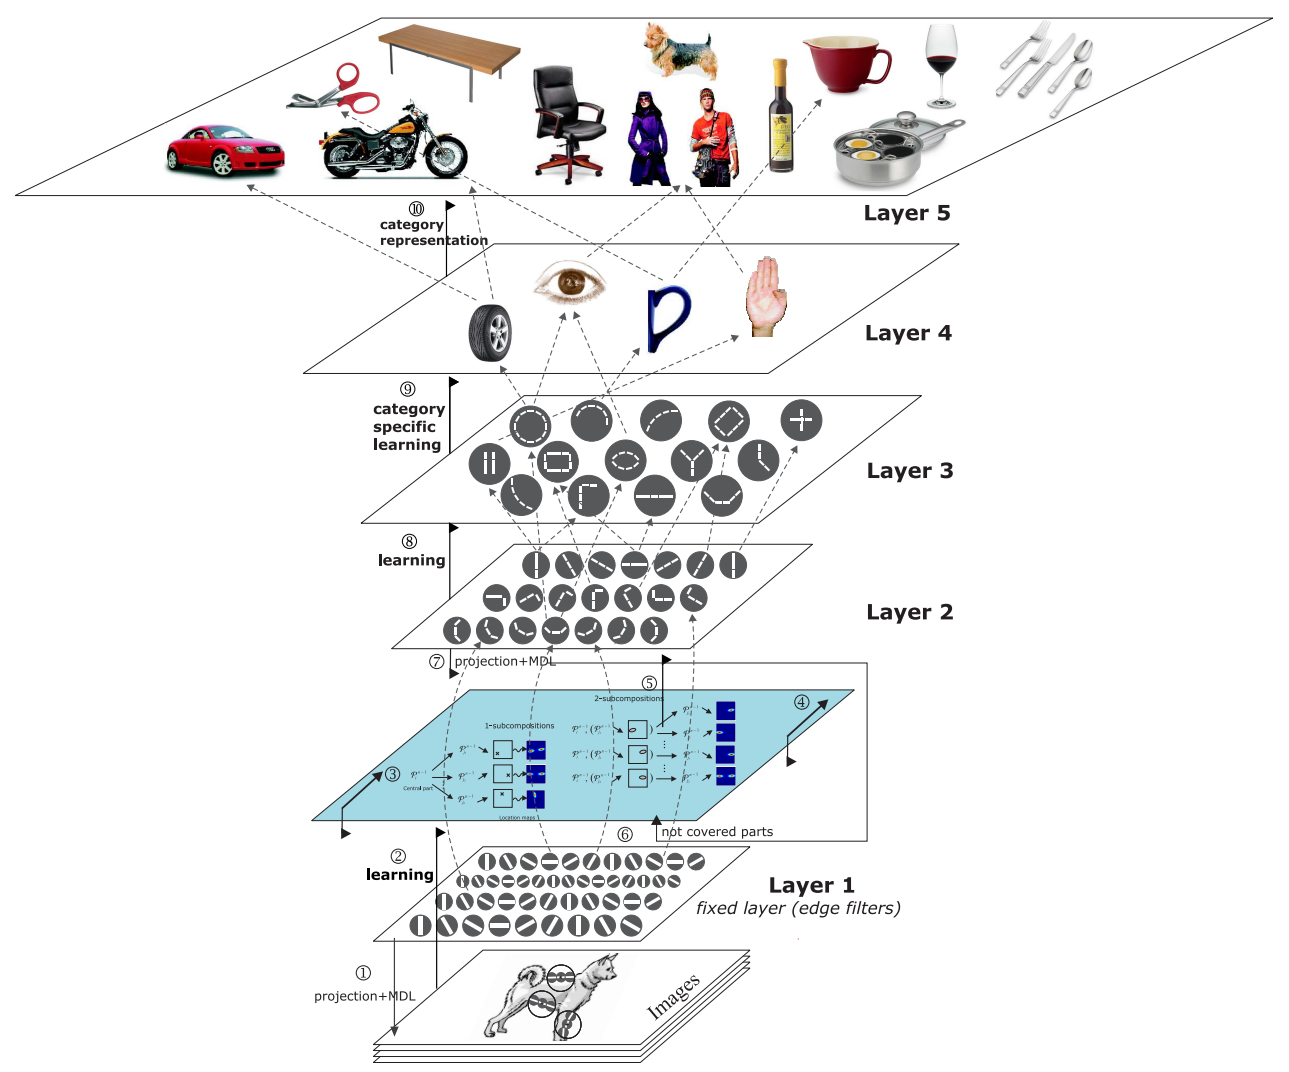
\includegraphics[scale=0.45]{backml/image-hierarchy.png}
  \caption{A custom hierarchical model illustrating the compositionnality and hierarchical nature of vision tasks (source: \parencite{leonardis2010learning}).}
  \label{fig:backml:hierarchy}
\end{figure}

Most of the \acrlong{ml} methods developed until recently can arguably be considered
``\textit{shallow}'' which means that they are not complex enough or their learning
process does not include a mechanism to learn or exploit such hierarchies. In
order to successfully apply these methods to complex data with hierarchical
structures, one usually needs to help the learning algorithm by pre-processing
the data and extracting meaningful information using field knowledge. This process
is called \textit{manual feature extraction} or \textit{engineering} and has been
an important part of the application of machine learning algorithms. In computer
vision, a great body of work has been focused on creating complicated pipelines
of feature extraction that produce hundreds of different features that can be used
for image understanding (\eg SURF \parencite{bay2006surf}, ORB \parencite{rublee2011orb}).
However, more recently ``\acrlong{dl}'' methods based on neural networks have
shown that manual feature extraction was usually not the best performing approach
for a wide variety of tasks.

Although neural network research is as old as machine learning itself, the real
breakthrough of \acrlong{dl} happened in 2012 at the occasion of the third iteration
of a \acrlong{ml} challenge called \acrfirstit{ilsvrc} \parencite{russakovsky2015imagenet}.
One of the tasks was image classification and all but the best method used
combinations of shallow learning algorithms and feature extraction. However, the
winning team followed a different approach. Building upon neural network research
form the previous decades, they used a deep convolutional neural network, AlexNet,
trained on the raw images directly \parencite{krizhevsky2012imagenet}. They beat
the second best method by a margin of 11\% error rate. This extraordinary improvement
revived the interest of the \acrlong{ml} community to neural networks and launched
the ``\acrlong{dl} revolution''. The success of this method can be partly attributed
to some particularily beneficial \textit{inductive bias}, a set of assumptions
that narrow the search of a good model in the hypothesis space. This inductive
bias includes the use of a trainable multi-layered (hence ``deep'') structure that
can automatically learn hierarchical concepts from the data directly. In other
words, instead of manual feature engineering, features are learned automatically.
Nowadays, \acrlong{dl} is a thriving research field that has grown far beyond
image classification. Section \ref{sec:backml:deeplearning} dives a little further
into \acrlong{dl} concepts relevant to this thesis.

\subsection{Transfer learning}
\label{ssec:backml:transfer}

As humans, we have extraordinary learning capabilites. Throughout our lives, we
learn to move, communicate, interact with our environments and more. One specific
learning ability that we possess is to use knowledge we have acquired in a given
context to learn faster in a different context. For example, someone who already
plays the violin will probably feel it easier to learn to play the piano than
someone who has no music education at all. In a way, we ``transfer'' knowledge
and skills from a task to another.

This idea has been applied in \acrlong{ml} and from this application emerged
\acrfirstit{tl} \parencite{yang2020transfer}. This field studies the ways knowledge
learned from one or more tasks, called the \textit{source tasks}, can be exploited
to learn more effectively on another task, the \textit{target task}. This subject
has been researched for few decades now, as the first contributions about \acrlong{tl}
date back to the end of the 1970s \parencite{bozinovski2020reminder}. A surge of
interest happened in the 1990s notably with a NIPS-95 workshop called
``\textit{Learning to Learn: Knowledge Consolidation and Transfer in Inductive Systems}''
which discussed the importance of retaining previously-learned information for
efficient learning. Since then, the interest has only been growing and the emergence
of \acrlong{dl} has created new opportunities for \acrlong{tl}.

Transfer learning methods are organized based on the properties of the source and
target tasks. The different types of supervision (or lack thereof) discussed in
Sections \ref{ssec:backml:sl} and \ref{ssec:backml:usl} also apply to \acrlong{tl}
in which case the supervision qualifier relates to the target task only. In other
words, in supervised \acrlong{tl}, the target task is a supervised dataset as
described in Equation \ref{eqn:backml:supervised}. For the remainder of the section,
we will assume that the source tasks are also supervised.

Transfer learning can be \textit{homogeneous} (see Definition \ref{def:backml:homotransfer})
when the source and target tasks only differ by the distributions of their data.
As an example, let us suppose we would want to classify pictures taken with a
camera equipped with a certain sensor (target dataset $B$) and that we also have
at hands another dataset of pictures taken with a camera equipped with another
type of sensor (source dataset $A$). Each captor has a certain noise pattern which
results in dataset $A$ and $B$ to have a slighlty different distributions in the
pixel intensities (\ie $p_A(x) \neq p_B(x)$). This specific setup where only the
inputs distributions differ is called \textit{domain adaptation}.

\begin{definition}
\label{def:backml:homotransfer}
Transfer learning between a source task $\left(\mathcal{X}_{s}, \mathcal{Y}_{s}, p_{s}(\vect{x}, y)\right)$ and a target task $\left(\mathcal{X}_t, \mathcal{Y}_t, p_t(\vect{x}, y)\right)$ is said to be \textbf{homogeneous} when $\mathcal{X}_s \cap \mathcal{X}_t \neq \emptyset$ and $\mathcal{Y}_s = \mathcal{Y}_t$ but $p_s(\vect{x}) \neq p_t(\vect{x})$ or $p_s(y|\vect{x}) \neq p_t(y|\vect{x})$.
\end{definition}

Transfer learning can be \textit{heterogeneous} (see Definition
\ref{def:backml:heterotransfer}). An example that will be addressed later in this
thesis is the transfer of a model trained for natural image classification to
medical image classification. In this case, the tasks are different as the first
consists in identifying the presence of a type of object in the image whereas the
other consists in assessing the malignancy of a tumor from an image of a tissue.
The input distributions also differ as medical images have completely different
content and appearance.

\begin{definition}
\label{def:backml:heterotransfer}
Transfer learning between a source task $\left(\mathcal{X}_{s}, \mathcal{Y}_{s}, p_{s}(\vect{x}, y)\right)$ and a target task $\left(\mathcal{X}_t, \mathcal{Y}_t, p_t(\vect{x}, y)\right)$ is said to be \textbf{heterogeneous} when $\mathcal{X}_s \cap \mathcal{X}_t = \emptyset$ and/or $\mathcal{Y}_s \neq \mathcal{Y}_t$.
\end{definition}

There exists many different transfer approaches. Based on how they operate,
\parencite{yang2020transfer} have identifed four different categories of \acrlong{tl}
algorithms. The case when knowledge transfered corresponds to the weights attached
to the source examples is called \textit{instance-based} \acrlong{tl}. Is referred
to as \textit{feature-based} \acrlong{tl} the case when knowledge is represented
by a subspace spanned by the features in the source and target domains. The
transferred knowledge can also be embedded as part of the source domain model:
this is \textit{model-based} \acrlong{tl}. Finally, when the knowledge is transferred
as rules specifying the relations between examples in the source domains, transfer
is referred to as \textit{relation-based}.

Transfer learning performance is influenced by serveral factors including how well
the method is able to capture and use transferable knowledge. The task-relatedness
is also an important factor: usually the more similar the tasks, the better the
performance. Sometimes, performance are worsen by the use of \acrlong{tl}. This
happens for instance when the source and target tasks are not related enough.
Moreover, the training process on the target task can cause some of the
previously-learned knowledge to be lost as most \acrlong{ml} methods do not have
an explicit memory mechanism to retain information. These two phenomena are
respectively called \textit{negative transfer} \parencite{zhang2020overcoming}
and \textit{catastrophic interference} \parencite{french1999catastrophic}. Although
some methods have been proposed to tackle these challenges, how to anticipate and
correct them are still open research questions.

We explore further \acrlong{tl} in the context of deep learning in Section
\ref{ssec:backml:dl:deeptransfer}.

\subsection{Multi-task learning}
\label{ssec:backml:mtl}

In \acrlong{tl}, the transfer process happens in two steps. First, knowledge is
extracted from the source tasks one way or another, then later used for learning
the target task. A similar approach is \acrfirstit{mtl} where, rather than performing
the transfer in two steps, everything happens at once: a model is trained on all
tasks simultaneously. Compared to learning each task individually, this approach
has several advantages: it increases the total amount of data available for training
a model, a more robust and universal representation can be learned by sharing
knowledge between tasks and, to a certain extent, it prevents the model to
overfit\footnote{See more on overfitting in Section \ref{ssec:backml:bvtradeoff}.}
a specific task. In the best scenarii, the use of \acrlong{mtl} improves the
performance of each individual task compared to a setup where the tasks are treated
independently. In opposition, it happens that antagonistic tasks worsen the
resulting individual tasks performance. This issue is related to negative transfer
and catastrophic interference introduced in Section \ref{ssec:backml:transfer}.

Similarily to \acrlong{tl}, \acrlong{mtl} methods can be either \textit{heterogeneous}
when the tasks are of different types (\eg supervised, unsupervised, classification,
regression), or \textit{homogeneous} when tasks have only one type. In supervised
\acrlong{mtl}, \parencite{zhang2017survey} have identified three families of
methods. \textit{Feature-based} \acrlong{mtl} is about sharing knowledge through
learning features common among all tasks. With \textit{instance-based} \acrlong{mtl},
knowledge is shared through examples deemed useful. Finally, \textit{model} or
\textit{parameter-based} \acrlong{mtl} use learned models as proxies to extract
information about tasks relatedness.

% ===================
% Eval and selection
% ===================

\section{Model evaluation and selection}
\label{sec:backml:modeleval}

As stated in Section \ref{sec:backml:whatisml}, evaluation is a core principle of
\acrlong{ml} as a learning algorithms should select a model that maximizes a
performance criterion. In this section, we introduce different concepts related
to the evaluation and selection of machine learning models. In Sections
\ref{ssec:backml:bvtradeoff} and \ref{ssec:backml:bvtradeoff}, we discuss the
importance of generalization for \acrlong{ml} models and the related topics of
bias-variance trade-off and overfitting. In Section \ref{ssec:backml:modelselection},
we discuss further practical consideration related to model selection. In Section
\ref{ssec:backml:metrics}, we finally introduce different metrics used in this
thesis.


\subsection{Empirical risk minimization}
\label{ssec:backml:modelselection}
As stated in the introduction, the objective of a learning algorithm is to find
a model $h \in \mathcal{H}$ that maximizes a performance measure or, alternatively,
minimizes the expected risk $R(h)$ (for a supervised problem)
\parencite{vapnik1992principles}:

\begin{equation}
\label{eqn:backml:expriskmin}
R(h) = \mathbb{E}_{\mathcal{X},\mathcal{Y}}\left\{\ell\left(h(\vect{x}), y\right)\right\}
\end{equation}

where $\ell: \mathcal{Y}\times\mathcal{Y} \rightarrow \mathbb{R}$ is a loss function
which measures the closeness between $h(\vect{x})$ and $y$. The expected risk is
also called the \textit{generalization error}. The model that minimizes $R(h)$ is
therefore the best possible model for the task and is called the Bayes model $h_B$.
In practice, it is rarely possible to directly minimize the expected risk as one
does not have access to the true distributions. It is therefore more convenient
to work with an unbiased estimator of the estimated risk, the empirical risk,
which is evaluated using the available supervised training set $\mathcal{S}$:

\begin{equation}
\label{eqn:backml:empiricalrisk}
R_e(h) = \frac{1}{n} \sum_{i=1}^{|\mathcal{S}|} \ell(h_\mathcal{S}(\vect{x}_i), y_i), (\vect{x}_i, y_i) \in \mathcal{S}
\end{equation}

The \acrfirstit{erm} principle suggests that a learning algorithm should pick a
model that minimizes the emprical risk in order to approximate $h_B$ as well as
possible. Most machine learning algorithms apply this principle.

\subsection{Bias-variance trade-off and overfitting}
\label{ssec:backml:bvtradeoff}

Whereas it can be shown that the empirical risk, under some assumptions, converges
to the expected risk when the training set grows ($n \rightarrow \infty$), in
practice, one does not have access to an infinitely-large dataset. Therefore, the
learned model will often differ from $h_B$ and its expected risk will often be
larger. The effect of the ``\textit{choice}'' of a finite training set on the
generalization error can be studied using the \textit{bias-variance decomposition}
\parencite{geman1992neural, geurts2009bias, friedman2017elements}:

\begin{equation}
\label{eqn:backml:biasvariancedec}
\mathbb{E}_{LS}\left\{\mathbb{E}_{\mathcal{X},\mathcal{Y}}\left\{ \ell(h_{LS}(\vect{x}), y)\right\}\right\} = \text{noise}(\vect{x}) + \text{bias}^2(\vect{x}) + \text{variance}(\vect{x})
\end{equation}

where $\mathbb{E}_{LS}$ is the expectation over all training sets of size $n$ that
can be extracted from $p(\vect{x},y)$ and $h_{\mathcal{S}} \in \mathcal{H}$ is
the model learned from a learning set $\mathcal{S} \in LS$. The \textit{noise}
term is the error of $h_B$ and is therefore irreductible. The \text{bias} is the
error of the average model (over models generated from $LS$) with respect to $h_B$.
The \textit{variance} measures the variability of the predictions around the
average model caused by the training set randomness. Several elements have a direct
impact on these error terms such as: model capacity, training set size, noise in
the data, \etc.

The \textit{capacity} or \textit{complexity} of a model is related to its ability
to capture complex relationships in the data. Linear models (see Section
\ref{sec:backml:svm}) are examples of low-capacity models as they are only able
to capture linear relationships. Non-linear models such as random forests (see
Section \ref{sec:backml:treebased}) or deep neural networks have a higher complexity
or capacity compared to linear models.

Low-capacity models usually have low variance as their limited expressiveness does
not allow them to change much based on the training data but they also have high
bias as failing to capture complex relationships prevents the model from approximating
$h_B$ correctly. This behavior is called \textit{underfitting}. In opposition,
high-capacity models have low bias as their expressiveness allow them to approximate
$h_B$ more accurately but this expressiveness also leads to high-variance as the
model can learn a function which is too expressive compared to $h_B$ and can fit
the noise in the training data. Such models suffer from \textit{overfitting} which
hampers generalization, although these models typically present a low empirical
risk. The \textit{bias-variance trade-off} results from these observations and
states that finding a model that generalizes consists in finding the trade-off
between low- and high-capacity or underfitting and overfitting. In Figure
\ref{fig:backml:biasvariancetradeoff} is plotted the classical representation of
this trade-off.

\begin{figure}
  \centering
  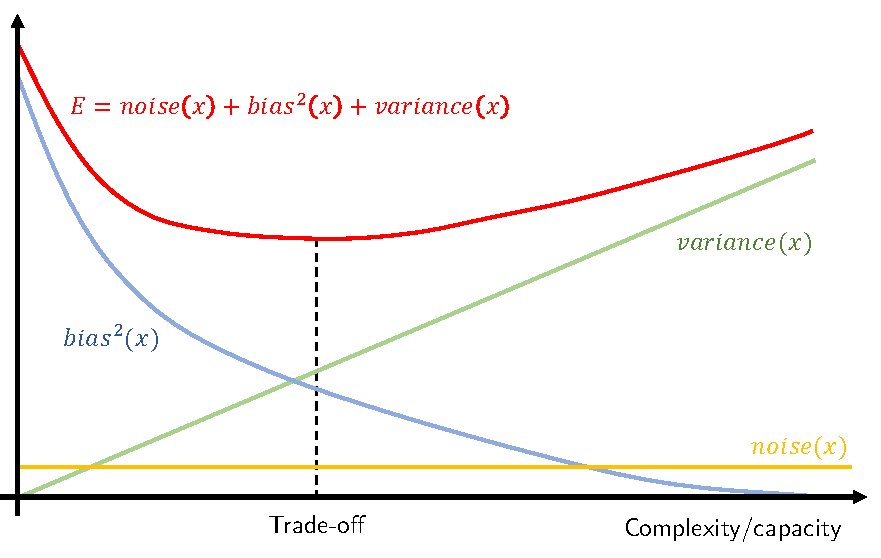
\includegraphics[scale=0.75]{backml/biasvariancetradeoff.pdf}
  \caption{The bias-variance trade-off illustrated.}
  \label{fig:backml:biasvariancetradeoff}
\end{figure}

\subsubsection{Over-parametrized models}

With the advent of \acrlong{dl}, model complexity has exploded as typical \acrlong{dl}
models have millions or even billons of parameters (see Section
\ref{ssec:backml:dl:modernarchi}). The bias-variance trade-off tells us that these
models should be extremely prone to overfitting but the reality is different.
Typically, it is not uncommon to find tasks for which \acrlong{dl} models reach
an empirical risk close to zero but actually generalize well to unseen data
\parencite{zhang2021understanding}. Although the models are able to basically
memorize the training data, the learned function is actually very robust and
generalize well. This phenomenon is currently being investigated and several
explanations have been proposed such as the deep double-descent
\parencite{belkin2019reconciling}.

\subsection{Model selection and evaluation in practice}
\label{ssec:backml:modelselinpractice}

These considerations have direct consequences on practical applications of machine
learning. In particular, the presence of overfitting causes the empirical risk to
reflect poorly the generalization error of a model. There are two common tasks
where using the empirical risk only is not reliable which are \textit{model selection}
and \textit{model evaluation}. The former consists in finding the model that would
generalize best among a set of candidates and the latter consists in evaluating
the expected performance of a model when it will be used on new data. Both tasks
involve evaluating the generalization of a model. There exists several approaches
to solve these tasks.

The simplest one is the use of an independant test set: the source dataset is
split into two subsets, the train and test sets, which are used to respectively
train and evaluate the model. The size of the subsets should be made such that
the train set is large enough for the model to be able to learn but the test set
should be large enough for the estimate of the error to be reliable. Those two
objectives are obviously antagonistic. Therefore, this approach is not viable if
the source dataset is too small as reducing even more the size of the sets will
make both the training and evaluation unreliable. The test-set approach actually
evaluates the generalization error of the model for the given dataset but not the
expected generalization error presented in Equation \ref{eqn:backml:biasvariancedec}.

Another approach that actually estimates the expected generalization error is
\acrfirstit{cv} which simply repeats the train-test approach with different splits
of the source dataset. For each train-test split, a model is trained on the train
set and evaluated on the test set. The \acrlong{cv} score is computed by averaging
the test scores of all splits. There exists several approaches for \acrlong{cv}
which differ by how they generate their splits. A common approach is
\textit{$k$-fold \acrlong{cv}} where the data is randomly split into $k$ subsets
and each subset is selected in turn to be the test set while the remaining folds
make the train set.

An important consideration is to never use a model selection score as the evaluation
score of a model. Indeed, optimizing the choice of a model usually results in the
selection score to be an overly optimistic estimator of the generalization
performance of the model. In practice, this results in a three-way split of the
training dataset: one extracts some train, validation and test sets. The models
are trained on the train set, selected on the validation set and the final model
is evaluated on the test set. When the dataset is too small for such a three-way
split, a common approach consists in extracting a test set from the whole dataset
and then performing \acrlong{cv} on the train set. As a general rule, every decision
influenced one way or another by the output $y$ should be done within a validation
loop to avoid overfitting (using either \acrlong{cv} or an independant
test-set).

These two approaches are based on a strong assumption that the extracted sets are
independant. If they are not, this would most probably lead to overfitting and
the resulting selection or evaluation scores being overly optimistic. Therefore,
it is sometimes not enough to split the sets randomly and domain knowledge must
be used during the splitting procedure to enforce sets independance. This issue
is sometimes called \textit{data leakage} \parencite{kaufman2012leakage} as
information ``leaks'' between the sets. This topic will be discussed in Section
\ref{sec:backdp:dataset} as \acrlong{dp} datasets must treated carefully to avoid
this issue.

\subsection{Metrics}
\label{ssec:backml:metrics}

% F1 ?
The metrics presented in this section are mostly supervised classification
performance measures. Given a supervised dataset as described in Equation
\ref{eqn:backml:supervised}, the metrics evaluate how the predicted class $\hat{y}_i$
compares to the ground truth class $y_i$. In the remainder of the thesis, when
the higher the better for a metric, we will call it a \textit{score}. In opposition,
when the lower the better, we will call it a \textit{loss}. In terms of notations,
a loss and a score computed over a set of data will respectively be noted
$\mathcal{L}$ and $\mathcal{M}$.

\subsubsection{Accuracy}
\label{sssec:backml:metric:acc}
The accuracy was introduced in our first example of a machine learning problem in
Section \ref{sec:backml:whatisml} with its dual, the zero-one loss. The accuracy
assigns 1 to correct predictions and 0 to misclassified samples. The accuracy
score can be computed over a dataset:

\begin{equation}
\label{eqn:backml:accuracy}
\mathcal{M}_{\text{acc}} = \dfrac{1}{n} \sum\limits_{i = 1}^n (1 - \ell_{\text{0-1}}(y_i, \hat{y}_i))
\end{equation}

It has the advantage of being simple to interpret, to compute and it applies to
both binary and multi-class problems. However, it is affected by \textit{class imbalance}.
This phenomenon designates the situation when there is a disparity in the numbers
of examples belonging to each of the problem classes in the dataset. For instance,
given binary dataset where $n-1$ examples belong to class $A$ and the last example
to class $B$, a classifier predicting only class $A$ would obtain an accuracy
close to $1$ which seems very good but in reality the classifier did not learn
anything from the data.

\subsubsection{Area under the ROC curve}
\label{sssec:backml:metric:rocauc}

In binary classification, a specific name is given to each type of successful or
unsuccessful predictions and these different types of successes and errors form
what is called the \textit{confusion matrix} (see Table \ref{tab:backml:confusion}).
Each element of this table can be either a number or a proportion of samples
falling in the category. The accuracy presented in Section \ref{sssec:backml:metric:acc}
can be re-expressed based on this confusion matrix: $\frac{TN + TP}{N + P}$. In
some context, however, it is more informative to look at other types of errors.
For instance, when the target task consists in diagnosing cancer, one is more
interested in assessing the number of false positives and negatives of the method
using, for instance, the \textit{specificity} or \textit{sensitivity} (\aka recall)
scores.

\begin{equation}
\label{eqn:backml:specifity}
\textit{Specifity} = \frac{TN}{TN + FP} = 1 - \frac{FP}{N}
\end{equation}

\begin{equation}
\label{eqn:backml:sensitivity}
\textit{Sensitivity} = \frac{TP}{P}
\end{equation}

\begin{table}
  \centering
  \begin{tabular}{c|cc|c}
  & \multicolumn{2}{c}{Predicted ($\hat{y}$)} & \\
  Actual ($y$) & 0 & 1 & Total \\
  \hline
  0 & \textbf{T}rue \textbf{N}egative & \textbf{F}alse \textbf{N}egative & \textbf{N}egative \\
  1 & \textbf{F}alse \textbf{P}ositive & \textbf{T}rue \textbf{P}ositive & \textbf{P}ositive \\
  \end{tabular}
  \caption{A confusion matrix for a binary classification problem.}
  \label{tab:backml:confusion}
\end{table}

\textit{Sensitivity} and $1 - \textit{specificity}$ are also called \acrfirstit{tpr}
and \acrfirstit{fpr} respectively. These metrics should always be studied together
as it is often possible to optimize one at the expense of the other. Therefore a
common analysis consists in plotting a model as a point $(\acrshort{tpr}, \acrshort{fpr})$
in a two-dimensional graph. Some classification models are able to produce class
probabilities instead of just a class. In this case, one can vary a threshold
applied to these probabilities in order to generate several points to plot. These
points form a visual metric called the \acrfirstit{roc} curve (see Figure
\ref{fig:backml:roc-curve}) which can be derived into a score: the
\textit{area under the \acrshort{roc} curve} (\rocauc). The drawbacks of this
score are that it can only be computed for model which produce a meaningfully
thresholdable number, it is relatively computationally expensive to obtain as one
have to evaluate all possible thresholds and it only applies to binary classification.
However, it provides a measure which is not impacted by class imbalance which is
a very interesting property in domains where this issue is common. Another advantage
of the the \rocaucs is its finer grasp of how a model performs as it evaluates
the probablities unlike the accuracy where the model is either wrong or right but
there is no in-between.

\begin{figure}
  \centering
  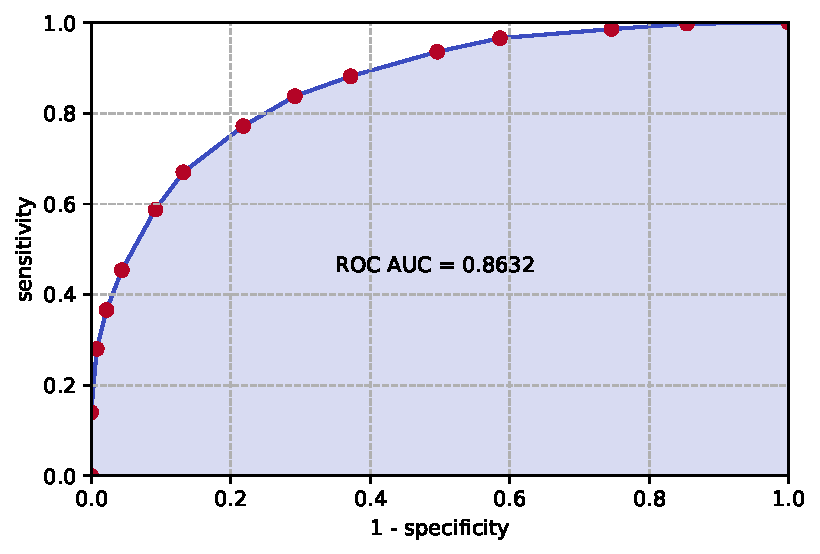
\includegraphics[scale=0.9]{backml/roc-curve.pdf}
  \caption{A \acrshort{roc} curve. The red points correspond to different threshold values applied to the probabilities produced by the model. The area of the light blue zone under the curve is the \acrshort{roc} \acrshort{auc} score.}
  \label{fig:backml:roc-curve}
\end{figure}


\subsubsection{Cross-entropy loss}
\label{sssec:backml:metric:crossentropy}

Cross-entropy is rooted in information theory and measures the similarity of two
probability distributions $p$ and $q$ that, when defined over a finite and discrete
set of events $\mathcal{X}$, is given by:
\begin{equation}
\label{eqn:backml:crossentropy}
H(p, q) = - \sum\limits_{x_i \in \mathcal{X}} p\left(x_i\right) \log q\left(x_i\right)
\end{equation}

When the model outputs class probabilities, this similarity measure can be used
to evaluate the discrepency between the prediction and the ground-truth. The
cross-entropy becomes a loss function called the
\textit{categorical cross-entropy}:
\begin{equation}
\label{eqn:backml:crossentropyloss}
\mathcal{L}_{ce} = - \frac{1}{n} \sum\limits_{i=1}^n \sum\limits_{c=1}^{\left|\mathcal{Y}\right|} y^{(c)}_{i} \log \hat{y}^{(c)}_i
\end{equation}
where $\hat{y}^{(c)}_i$ is the probability predicted by the model for example $i$
and class $c$ and $y^{(c)}_i$ is the one-hot encoding of the ground truth:
\begin{equation}
\label{eqn:backml:onehotencoding}
y^{(c)}_i =
\begin{cases}
1,\,\text{if}\, y_i = c \\
0,\,\text{otherwise}
\end{cases}
\end{equation}

In the case of binary classification, the metric falls back to the
\acrfirstit{bce}:
\begin{equation}
\label{eqn:backml:bce}
\mathcal{L}_{bce} = - \frac{1}{n} \sum\limits_{i=1}^n \left(y_i \log \hat{y}_1 + (1 - y_i) \log (1 - \hat{y}_i)\right)
\end{equation}

Similarly to \rocauc, the cross-entropy evaluates probabilities and therefore has
a fine grasp on how the model performs. Another important advantage is its
differentiability as it can be used as a loss for directly training differentiable
models (\eg \acrlong{dl} models, see Section \ref{ssec:backml:dl:opti}).

\subsubsection{Dice score}
\label{sssec:backml:metric:dice}

As opposed to the previous metrics, the dice score is a set similarity measure
that is used to evaluate binary image segmentation. Considering two sets $\mathcal{A}$
and $\mathcal{B}$, the dice score is defined as:
\begin{equation}
\label{eqn:backml:diceAB}
\mathcal{D} = \frac{2 \left|\mathcal{A}\cap \mathcal{B}\right|}{\left|\mathcal{A}\right| + \left|\mathcal{B}\right|}
\end{equation}
When working with image segmentation, $\mathcal{A}$ and $\mathcal{B}$ become the
sets of true and predicted binary labels for the pixels in the image and the
intersection falls back to a dot product. The resulting formula is:
\begin{equation}
\label{eqn:backml:dice}
\mathcal{M}_{dice} = \dfrac{2 \sum_i\sum_j y_{ij} \hat{y}_{ij} + \epsilon}{\sum_i\sum_j y_{ij} + \sum_i\sum_j \hat{y}_{ij} + \epsilon}
\end{equation}
where $\epsilon$ is a small value added for numerical stability, $y_{ij}$ is the
actual class of pixel $(i, j)$ and $\hat{y}_{ij}$ the predicted class for this
pixel. The predicted $\hat{y}_{ij}$ can either be binary or a probability. In the
latter case, the metric is called the \textit{soft dice score} which is differentiable.
When the model outputs class probabilities, instead of using the soft dice score,
$\hat{y}_{ij}$ can be binarized using a threshold.

\subsubsection{Rankings of metrics}
\label{ssec:backml:metric:rankings}

In Part \ref{part:transfer} of this thesis, we use a relatively large set of image
classification datasets to study \acrlong{tl}. In order to compare the different
methods, we evaluate how it performs on those datasets. Unfortunatly, for reasons
that will be explained later, it is not possible to use the same metric for all
datasets. Moreover, a metric computed on a dataset is not always comparable to
the same metric computed on a different dataset. For this reason, we resort to
using \textit{rankings of methods}. First, for each dataset in our pool, we evaluate
the methods each with their most appropriate metric and then rank them: the best
method gets rank 1 and the worst gets rank $m$ (where $m$ is the number of methods).
Finally, in order to draw general conclusions, we average the rankings over all
the datasets. The average ranks therefore provides a single metric for comparing
the methods across datasets. This metric is not ideal
\TODO{rankings are apparently unstable metrics, would like to discuss it more but haven't found any source yet discussing the issue.}.

% ===================
% Methods
% ===================

\section{Support vector machines}
\label{sec:backml:svm}

The \acrfirstit{svm} algorithm was invented in the early 1990s \parencite{boser1992training}.
It is originally a linear method that can be used for regression and classification.
By using the \textit{kernel trick}, \acrshort{svm} can also learn non-linear models
but it is out of the scope of this thesis. An interested reader will learn more
about kernel methods and the kernel trick in \parencite{friedman2017elements}.

In general, assuming a supervised dataset where inputs are such that
$\vect{x} \in \mathbb{R}^m$ where $m$ is the number of features, a linear model
is an hyperplane:

\begin{equation}
\label{eqn:backml:linearmodel}
f(\vect{x}) = \theta_0 + \sum_{j=1}^m \theta_j x_j
\end{equation}

where $\theta_0$ and the $\theta_j$ are the learnable parameters, respectively
called the \textit{bias} and the \textit{weights}. This model can be used for
regression in which case the model $h(\vect{x}) = f(\vect{x})$. A linear model
can also be used for binary classification in which case the linear function is
called the \textit{decision boundary} and is considered to separate positive from
negative samples in the input space: $h(\vect{x}) = \text{sign}(f(\vect{x}))$ (\ie
$\mathcal{Y} = \left\{-1, 1\right\}$). Linear methods differ from each other by
the way they learn and generate these weights.

Support vector machines optimize the parameters $\theta_0$ and $\theta_j$ to
generate $f$ in such a way that the minimal distance from the hyperplane to the
nearest points from the learning set is maximized. These nearest points are called
the \textit{support vectors} and the margin between the support vectors is called
the \textit{gutter}. An example of a \acrshort{svm} hyperplane is given in Figure
\ref{fig:backml:svm}. It can be shown that the \acrshort{svm} optimization problem
falls back to the Lagrange dual:

\begin{align}
\label{eqn:backml:svmoptimizationproblem}
\underset{\boldsymbol{\alpha}}{\text{max}}& \sum_{k=1}^n \alpha_k - \frac{1}{2} \sum_{i,j=1}^n \alpha_i\alpha_j y_i y_j \vect{x}_i^T \vect{x}_j \\
\text{subject to}~& 0 \leq \alpha_k \leq C, \forall k = 1, ..., n \\
& \sum_{i=1}^n \alpha_i y_i = 0
\end{align}

which can be solved efficiently with classical linear solvers such as LIBLINEAR
\parencite{fan2008liblinear}. When the optimal solution has been found, the weights
can be derived by solving the system:

\begin{equation}
\label{eqn:backml:svmweights}
\alpha_k\left(y_k \left(\theta^T \vect{x}_k + b\right) - 1\right) = 0, \forall k = 1, ..., n
\end{equation}

In Equation \ref{eqn:backml:svmweights}, $\alpha_k > 0$ for the support vectors
$x_k$ and $\alpha_k = 0$ for the other samples. This is an interesting property
as it implies that only the support vectors and their weights $\alpha_k$ should
be stored for future inference. This makes the model very memory efficient for
problems where $m \gg n$. This property has also a negative side effect as it
means that the model is highly dependent on the support vectors $x_k$. It can
therefore change significantly if the $x_k$ are removed or changed which yields
high variance.

The $C$ term in the Lagrange dual formulation is an hyperparameter that relaxes
the need for linear separability of the training data and allows for training
examples to lie within the gutter or to be misclassified. Low values of $C$ make
the optimal solution tolerate more of such examples. Reducing the dependency of
the model on very few points also decreases the variance but increases the bias.
In opposition, high values of $C$ puts a large penalty on points that lie withing
the gutter or are misclassified which increases variance but decreases bias.

\begin{figure}
  \centering
  \subfloat[$C=10000$]{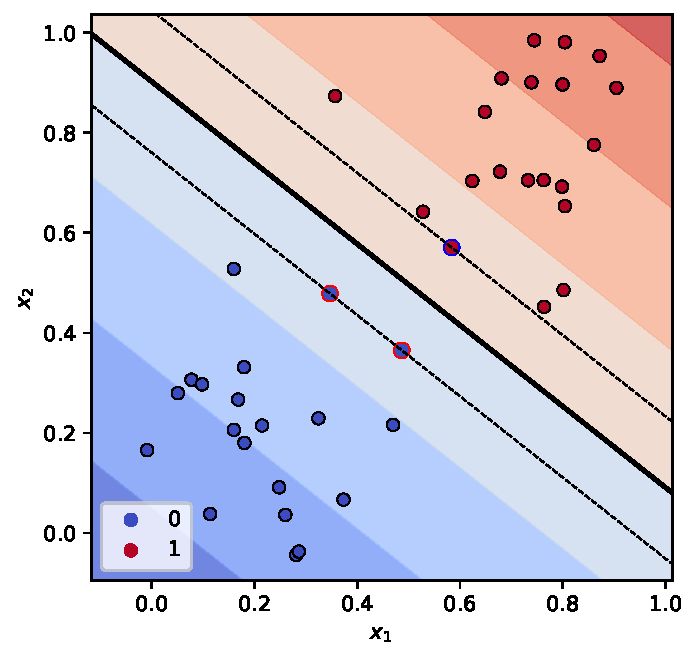
\includegraphics[scale=0.65]{backml/svm_c10000.pdf}}
  \subfloat[$C=25$. Notice the new points \\ of class $1$ in the class $0$ cluster.]{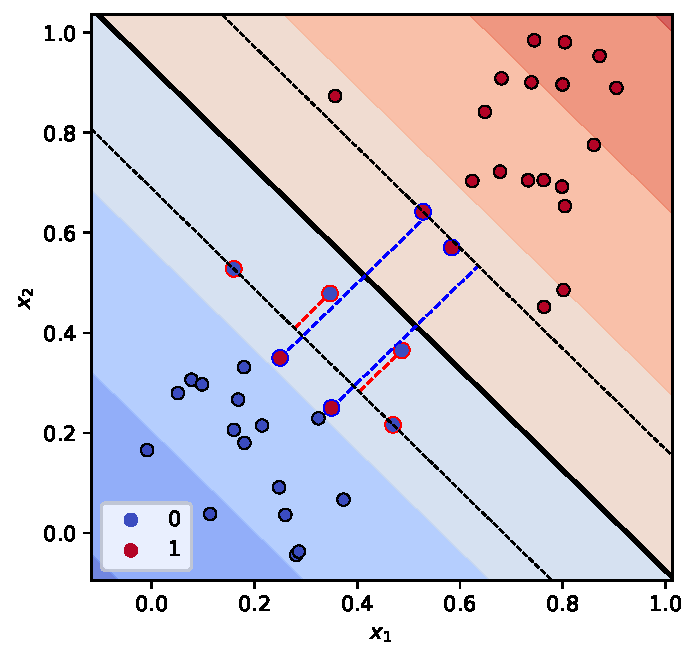
\includegraphics[scale=0.65]{backml/svm_c25.pdf}}
  \caption{Examples of an hyperplane (the thick black line) learned with \acrshort{svm} applied to a binary classification task ($\vect{x} = (x_1, x_2) \in \mathcal{X} \subseteq \mathbb{R}^2$ and $\mathcal{Y} = \left\{0, 1\right\}$). The support vectors are delineated with bold coloured border. A large value of $C$ penalizes more severely points in the gutter or misclassified.}
  \label{fig:backml:svm}
\end{figure}


\subsection{Multi-class problems}

There exists few approaches to use a binary classification algorithm like
\acrshort{svm} in a multi-class context. One of them is called \acrfirstit{ovo}
and consists in training $K=\frac{C(C-1)}{2}$ binary classifiers (where $C$ is
the number of classes), one for each pair of classes of the dataset. The prediction
for a new sample will be the majority class among the predictions of these $K$
models. This requires learning a model number quadratic with regard to the number
of classes. When C is large, this can be quite inefficient.

Another approach is called \acrfirstit{ovr} and consists in training $C$ models
each of which deals with the classification problem of a class versus all the
others. The final prediction is given by the model of which the decision function
returned largest value. This approach is more computationally efficient than
\acrshort{ovo} as only $C$ classifier have to be trained.

\section{Tree-based methods}
\label{sec:backml:treebased}

Tree-based methods are a popular family of methods invented at least twice in the
1980s by the \acrshort{ai} \parencite{quinlan1986induction} and the statistics
\parencite{breiman2017classification} communities. Section \ref{ssec:backml:dt}
presents the basics of decision tree inference and induction, Section \ref{ssec:backml:rf}
introduces the random forest algorithms. Section \ref{ssec:backml:et} presents a
variant of the random forest called \acrfirstit{et} and Section \ref{ssec:backml:et_image}
finally explores how this method can be used for image classification.

\subsection{Decision trees}
\label{ssec:backml:dt}

Let us consider a supervised dataset where each $\vect{x}_i$ is a vector of
attributes:
\begin{equation}
\label{eqn:backml:dt:vectattributes}
\vect{x}_i = \left(a^{(i)}_1, a^{(i)}_2, ..., a^{(i)}_m\right),~a^{(i)}_j \in \mathcal{X}_j
\end{equation}
and each attribute can be either numerical or categorical (binary or multi-valued).
A decision tree is a model structured as a tree of which the nodes $\mathcal{Q}$
are divided in two subsets: the internal and leaf nodes $\mathcal{I} \subset \mathcal{Q}$
and $\mathcal{F} \subset \mathcal{Q}$. Each internal node $q \in \mathcal{I}$
tests an input attribute $k_q \in \left\{1,...,m\right\}$ and its $E_q$ outwards
edges are associated with non-overlapping subsets of this attribute's domain:
\begin{equation}
\label{eqn:backml:dt:splitsgeneric}
\mathcal{A}^{(q)}_l \subset \mathcal{X}_{k_q},~l = 0,...,E_q-1
\end{equation}
which are called \textit{splits}. A leaf node of the tree is labelled with a
prediction $\hat{y} \in \mathcal{Y}$. In classification, it can also be a probability
distribution over $\mathcal{Y}$. In regression, the output is a real value
$\hat{y} \in \mathcal{Y}$. Given $x_i$, predicting an output value consists in a
top-down traversal of the tree. When reaching an internal node $q$ during the
traversal, $\vect{x}_i$ will follow the edge $l$ such that $a^{(i)}_{k_q} \in \mathcal{A}^{(q)}_l$
which leads to one of the children nodes of $q$. This process is repeated until
the algorithm reaches a leaf of which the associated labelling is the output of
the algorithm for $\vect{x}_i$.

In the remainder of the thesis, we will only consider numerical attributes and
binary splits at each internal node ($E_q = 2$). These splits are defined by a
threshold $v_q$ such that:
\begin{align}
\label{eqn:backml:dt:splitsbinary}
\mathcal{A}^{(q)}_0 &= \left]-\infty, v_q\right]\\
\mathcal{A}^{(q)}_1 &= \left]v_q, +\infty\right[
\end{align}
This representation allows for an efficient check at each node as the attribute
has just to be compared to the treshold. The inference algorithm is formalized in
Algorithm \ref{algo:backml:dtinference} for classification with numerical
attributes.

\begin{algorithm}[t]
  \SetAlgoLined
  \KwData{A sample $\vect{x}_i = \left(a^{(i)}_1, a^{(i)}_2, ..., a^{(i)}_m\right)$ and the root $r$ of a decision tree.}
  \KwResult{A probability distribution over $\mathcal{Y}$, the prediction for $\vect{x}_i$.}
  \SetKwFunction{dtinfer}{TreeInference}
  \Fn{\dtinfer{$r$, $\vect{x}_i$}}{
    $q = r$\;
    \While{$q \not\in \mathcal{F}$}{
      \eIf{$a^{(i)}_{k_q} \leq v_q$}{
        $q = q.\text{left}$\;
      }{
        $q = q.\text{right}$\;
      }
    }
    \KwRet{$q.\text{pred}$}\;
  }
  \caption{Inference with a classification tree and numerical attributes. $q.\text{left}$ and $q.\text{right}$ denote the left and right children of a node $q$ and the prediction associated with the leaf node $f \in \mathcal{F}$ is accessed through $f.\text{pred}$. The regression algorithm only differs by its type of output.}
  \label{algo:backml:dtinference}
\end{algorithm}

\subsubsection{Decision tree induction}
\label{sssec:backml:dtinduction}

Top-down tree induction is the name of the process of building a decision tree
from a supervised dataset. It is a greedy algorithm that, for a node and a set of
examples $S$, will select an attribute and a split which reduce the most the
so-called \textit{impurity} of the node. Then, $S$ will be divided in two subsets
$S_0$ and $S_1$ based on the selected split and these will be used to build
recursively the left and right sub-trees respectively. This procedure is repeated
until a certain stopping criterion is met. An impurity measure $I(S)$ evaluates
the disparity of the output labels $y_i$ in a set $S$ of training examples. For
classification, a common impurity measure is the Shannon entropy computed on the
class frequencies $p_i$:
\begin{equation}
\label{eqn:backml:shannon_entropy}
I(S) = - \sum_{i=1}^C p_i \log p_i
\end{equation}
The simplest stopping criterion would be to stop developing the tree when the
subset at the node cannot be further divided because either it is pure (\eg only
one class represented in $S$) or because all attributes have a constant value.
This algorithm is formalized in Algorithm \ref{algo:backml:dtinduction}.


\begin{algorithm}[t]
  \SetAlgoLined
  \SetKwFunction{dtinduct}{TreeInduction}
  \SetKwFunction{stopsplit}{StopSplit}
  \SetKwFunction{computepred}{ComputePred}
  \KwData{A  supervised dataset $S$ where each sample $\vect{x}_i = \left(a^{(i)}_1, a^{(i)}_2, ..., a^{(i)}_m\right)$.}
  \KwResult{The root node of a decision tree built for $S$.}

  \Fn{\dtinduct{$S$}}{
    \If{\stopsplit($S$)}{
      \KwRet{\text{a node associated with most appropriate labelling given} $S$}\;
    }
    Find the best split $v_q$ for attribute $k_q$ for new node $q$:\;
    $\argmin{v,k} \left[\frac{|S_0|}{|S|} I\left(S_0\right) + \frac{|S_1|}{|S|} I\left(S_1\right)\right] : S_0 = \left\{(\vect{x}_i, y_i) \mid a^{(i)}_k < v\right\}, S_1 = S \setminus S_0 $\; \label{algo:backml:dtinduction:argmax}
    $q.\text{left} =~$\dtinduct{$S_0$}\;
    $q.\text{right} =~$\dtinduct{$S_1$}\;
    \KwRet{$q$}\;
  }
  \;
  \Fn{\stopsplit{$S$}}{
    \KwRet{$true~$\text{if either the $y_i$ or all the attributes are constant in} $S$, $false~$\text{otherwise}}\;
  }
\caption{Decision tree induction.}
\label{algo:backml:dtinduction}
\end{algorithm}

\begin{figure}
  \centering
  \subfloat[Fully-developped]{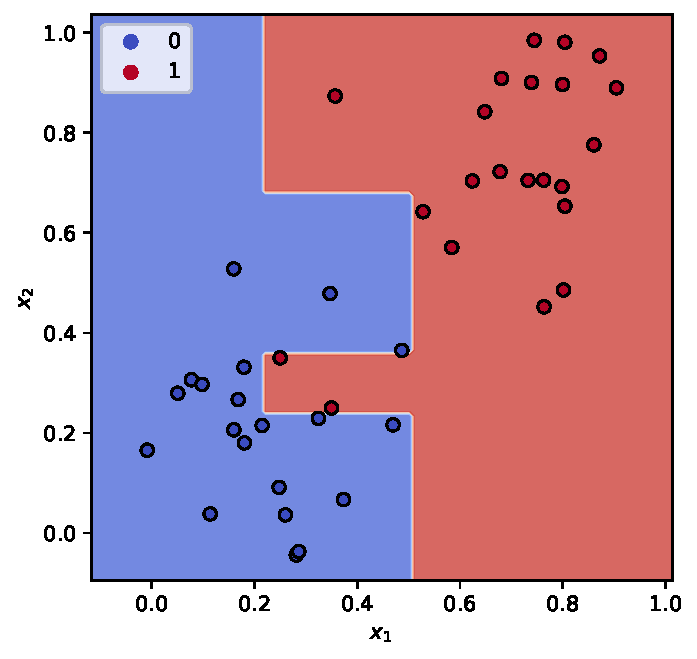
\includegraphics[scale=0.65]{backml/dt_full.pdf}}
  \subfloat[Maximum depth = 3]{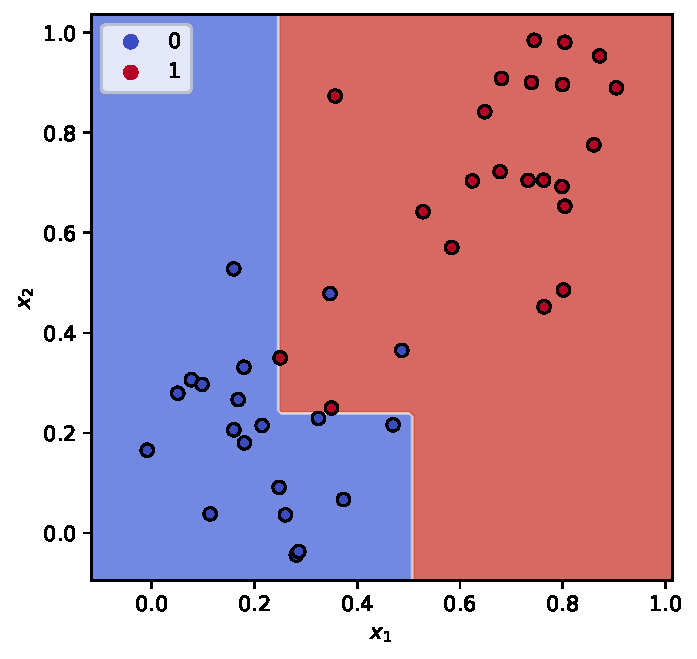
\includegraphics[scale=0.65]{backml/dt_max_depth3.pdf}}
  \caption{Decision tree decision boundary (white line). Pre-pruning using the maximum depth parameter reduces the complexity of the model.}
  \label{fig:backml:dt_boundary}
\end{figure}

A tree built using this simple stopping criterion is said to be \textit{fully-developed}.
Such a tree is able to capture the training set perfectly which, in practice,
hurts generalization as it usually leads to overfitting. In order to alleviate
the problem and reduce the variance, there exists several methods such as pre-pruning
which consists in preventing the final tree to grow too deep. Simple pre-pruning
techniques are, for example, stopping the induction when a branch reaches a certain
depth, or ensuring that all leaf nodes contain at least a given number of samples
(see Figure \ref{fig:backml:dt_boundary}). An advantage of decision trees are
their interpretability as the rules learned by the model can be easily understood
by looking at the tree. In practice, decision trees are rarely used alone because
of their high variance.

\subsection{Random forests}
\label{ssec:backml:rf}

Random forests \parencite{breiman2001random} is an ensemble method based on decision
trees. Ensemble methods combine the predictions of several models to produce a
final prediction. Random forest is part of the family of averaging techniques
where models are built independently and their predictions are averaged (\eg a
majority vote for classification). It can be shown that this approach reduces
variance compared to that of the base model (\eg decision trees) and the more
decorrelated the individual models, the more the variance reduction.

In random forests, decorrelation is achieved through \textit{bagging} (\aka
bootstrap aggregating) and \textit{random attribute subset selection}. The former
consists in training each individual model on a bootstrap sample of the training
set: the training set for the $t^{\text{th}}$ decision tree in the ensemble is a
set $S_t$ built by sampling $n$ examples with replacement from the original training
set $S$. Regarding the attribute subset selection, each tree only considers a
subset of $K \in \left\{1,..., m\right\}$ randomly selected features when looking
for the best split. In other words, only $K$ random features are considered when
searching for $k_q$ at line \ref{algo:backml:dtinduction:argmax} in Algorithm
\ref{algo:backml:dtinduction}. These two sources of randomness usually increase
the bias as the individual models do not have access to all the original training
examples and attributes. However, the variance reduction resulting from ensembling
is usually of much greater magnitude resulting in a significant performance
improvement compared to using a decision tree alone.

\subsection{Extremely randomized trees}
\label{ssec:backml:et}

The \textit{\acrlong{et}} (\acrshort{et}, \aka extra-trees) \parencite{geurts2006extremely}
are a variant of the random forests algorithm and introduces yet another source
of decorrelation by selecting the split $v_q$ at random during the induction
(instead of optimizing it, see line \ref{algo:backml:dtinduction:argmax} in
Algorithm \ref{algo:backml:dtinduction}). Moreover, to attenuate the bias increase,
each individual tree is built on the whole training set instead of a boostrap
sample. These choices makes the algorithm particularily computationally efficient
as it is not necessary to iterate over the training samples to optimize the split
anymore.

\subsection{Image classification with extra-trees}
\label{ssec:backml:et_image}

Extra-trees can be used for image classification as presented in \parencite{maree2016towards}.
The core idea behind this algorithm is to represent an image as a set of $n_w$
random subwindows. Subwindows are rectangle patches extracted from the image,
resized to have all the target height $t_r$ and width $t_c$ and flattened into a
vector of dimension $t_r \times t_c \times b$ ($b$, the number of color channels,
or bands, in the image). The original dimensions of the rectangular patches are
drawn uniformly at random in a range of proportions $s_{min}$ and $s_{max}$ of
the image size ($0 <= s_{min} < s_{max} <= 1$). The position of the patches are
also drawn uniformly at random. Each subwindow is attributed the class of its
parent image. The resulting training dataset containing $n \times n_w$ examples,
each a vector of dimension $t_h \times t_w \times c$, can be used to train an
extra-trees classifier. At inference, the same extraction process is applied and
the final prediction for the image is determined by a majority vote on the predicted
classes for its subwindows. Regarding parameters, the more windows and the more
trees in the forest, the better. In addition to the tree complexity hyperparameters,
the image colorspace, $s_{min}$ and $s_{max}$ should be tuned as well to optimize
generalization.

This variant of the algorithm is called \acrfirstit{etdic} but another variant
exists where the forest is used as a feature-learner (\acrshort{etfl}). The idea
of \acrshort{etfl} is to train a limited number of trees with the subwindows
dataset similarly to the \acrshort{etdic} approach. But rather than using the
forest as a direct classifier, it is used to create a new representation for the
images. This representation is a vector of the same dimension as the number of
leaves in the forest and value $\nu_i$ for leaf $i$ corresponds to the frequency
of subwindows of the image reaching the leaf when propagated into the forest. This
representation can then be used to train another classifier like \acrshort{svm}.
At inference, the representation for the new samples is extracted from the forest
which are then classified with the second classifier. In general, \acrshort{etfl}
is superior to \acrshort{etdic} in terms of performance.

\section{Deep learning}
\label{sec:backml:deeplearning}

As introduced in Section \ref{ssec:backml:shallowdeep}, \acrlong{dl} is a broad
research field that has grown rapidly since the breakthrough of AlexNet in 2012.
It encompasses many different research topics covering all areas of machine
learning. In this section, we dive a little further in \acrlong{dl} concepts and
methods relevant to this thesis. We introduce the basic components of modern neural
network architectures in Section \ref{ssec:backml:dp:components}. Section
\ref{ssec:backml:dl:opti} discusses how neural networks are learned and optimized
in practice. Section \ref{ssec:backml:dl:modernarchi} presents few modern neural
network architectures. Finally, in Section \ref{ssec:backml:dl:deeptransfer}, we
discuss deep \acrlong{tl}.

\subsection{Components of modern neural networks}
\label{ssec:backml:dp:components}

A feedforward neural network can be seen as a parametrized function approximator
$h$ which combines several intermediate functions $h^{(l)}(\cdot, \theta^{(l)})$
($l=1, ..., L$), also called \textit{layers}, through composition:
$h(\vect{x}, \theta) = (h^{(1)} \circ h^{(2)} \circ ... \circ h^{(L)})(\vect{x})$.
$\theta$ is the set containing all the learnable parameters of the neural network
$h$ and $\theta^{(l)}$ are the parameters of the function $h^{(l)}$ (or layer
$l$). The feedforward nature of the network specifies that information only flows
one-way, from the input $\vect{x}$ to the output $y$. In other words, there is no
feedback loop.

Unlike decision trees, for instance, which learn the tree structure automatically,
the architecture of a neural network is built manually (most of the time) and
consists in choosing and combining the appropriate functions $h^{(l)}$ for the
task at hand. Although it introduces some complexity when it comes to finding the
best architecture for a problem, this modularity actually offers a unprecedented
way of approaching model design as an engineering porblem and implementing inductive
bias. Moreover, as long as the chosen functions are differentiable, the final
network can be trained using the \textit{backpropagation} algorithm (see Section
\ref{ssec:backml:dl:opti}) independently of the architectural choices.

The idea behind one of the first machine learning algorithm ever published, the
perceptron \parencite{rosenblatt1958perceptron}, is still at the core of most
\acrlong{dl} architectures today. Loosely modeling the working of brain neurons,
the perceptron can be represented as:
\begin{equation}
\label{eqn:backml:perceptron}
f(\vect{x}) = \sigma\left(\theta_0 + \sum_{i=0}^m \theta_i x_i\right)
\end{equation}
where $\sigma(\cdot): \mathcal{X} \rightarrow \mathbb{R}$ is a non-linear
differentiable function called the \textit{activation function}, $\theta_0$ and
$\theta_i$ are respectively the learnable bias and weights. An eligible function
for $\sigma(x)$ should have at least two modes transitioning around $x=0$. In the
past decades, typical $\sigma$ functions were the hyperbolic tangent, the sigmoid
or the step function. Nowadays, the most common is the \acrfirstit{relu} function
(see Equation \ref{eqn:backml:relu}) which is particularily efficient to compute
and has some properties that interacts favorably with the training algorithm making
neural networks easier to train.

\begin{equation}
\label{eqn:backml:relu}
\sigma(x) = \text{ReLU}(x) = \begin{cases}
0\text{, if}~ x < 0\\
x\text{, else}
\end{cases}
\end{equation}

The perceptron, or \textit{neuron}, is simply a linear model and is therefore not
complex enough for many type of tasks. However, perceptrons can be combined together
into a perceptron layer: a parallel combination of $f$ perceptrons ($f$ is the
width of the layer) each with their own set of weights and biases and all taking
the same vector as input. A perceptron layer therefore outputs a vector
$\vect{z} \in \mathbb{R}^f$.

In the spirit of learning a hierarchy, perceptron layers can be connected one
after another to form a \acrfirstit{mlp} (see Figure \ref{fig:backml:mlp}). It
can be shown that sufficiently complex \acrshort{mlp}s are universal function
approximators (\ie they can learn any function) \parencite{hornik1989multilayer}
which is an interesting property. However, realistically dimensioned \acrshort{mlp}s
have the drawback of being very complex models easily reaching millions or even
billions of learnable parameters. This makes them difficult to optimize and prone
to overfitting. Regularization techniques exist to reduce model complexity such
as weight decay (\ie smaller absolute weights values are preferred over large
ones) or dropout \parencite{srivastava2014dropout} (\ie during training, some
neurons are disabled at random) but unfortunately are often not enough. Therefore,
whereas \acrshort{mlp}s still have their use in some applications and or as part
of larger and more diverse architectures, they are rarely used by themselves
nowadays.

\begin{figure}
  \centering
  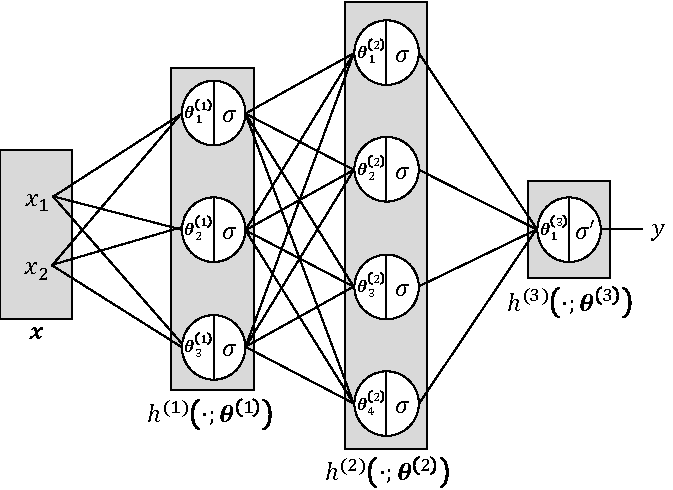
\includegraphics[scale=1]{backml/mlp.pdf}
  \caption{A \acrlong{mlp} with 2 hidden layers $h^{(1)}$ and $h^{(^2)}$ for a two-dimensional input $\vect{x}$.}
  \label{fig:backml:mlp}
\end{figure}

\subsubsection{Convolutional neural networks}
\label{sssec:backml:dl:cnn}

As introduced in Section \ref{ssec:backml:shallowdeep}, \textit{\acrlong{cnn}s}
(\acrshort{cnn}) are the origin of the ``\acrlong{dl} revolution''. Despite the
recently-revived interest, \acrshort{cnn}s have been reasearched since the late
1980s \parencite{lecun1989handwritten}. A \acrshort{cnn} is a network containing
at least one convolutional layer. Nowadays, such layers are a core component of
all networks processing structured data (time series, images, video, etc). For
instance, in image classification, typical architectures (see Figure \ref{fig:backml:cnn})
stack several convolutional and pooling layers followed by a fully-connected
network (\ie a \acrshort{mlp}). The convolutional layer is introduced in this
section and the pooling layer in Section \ref{sssec:backml:poolinglayer}.

\begin{figure}
 \centering
 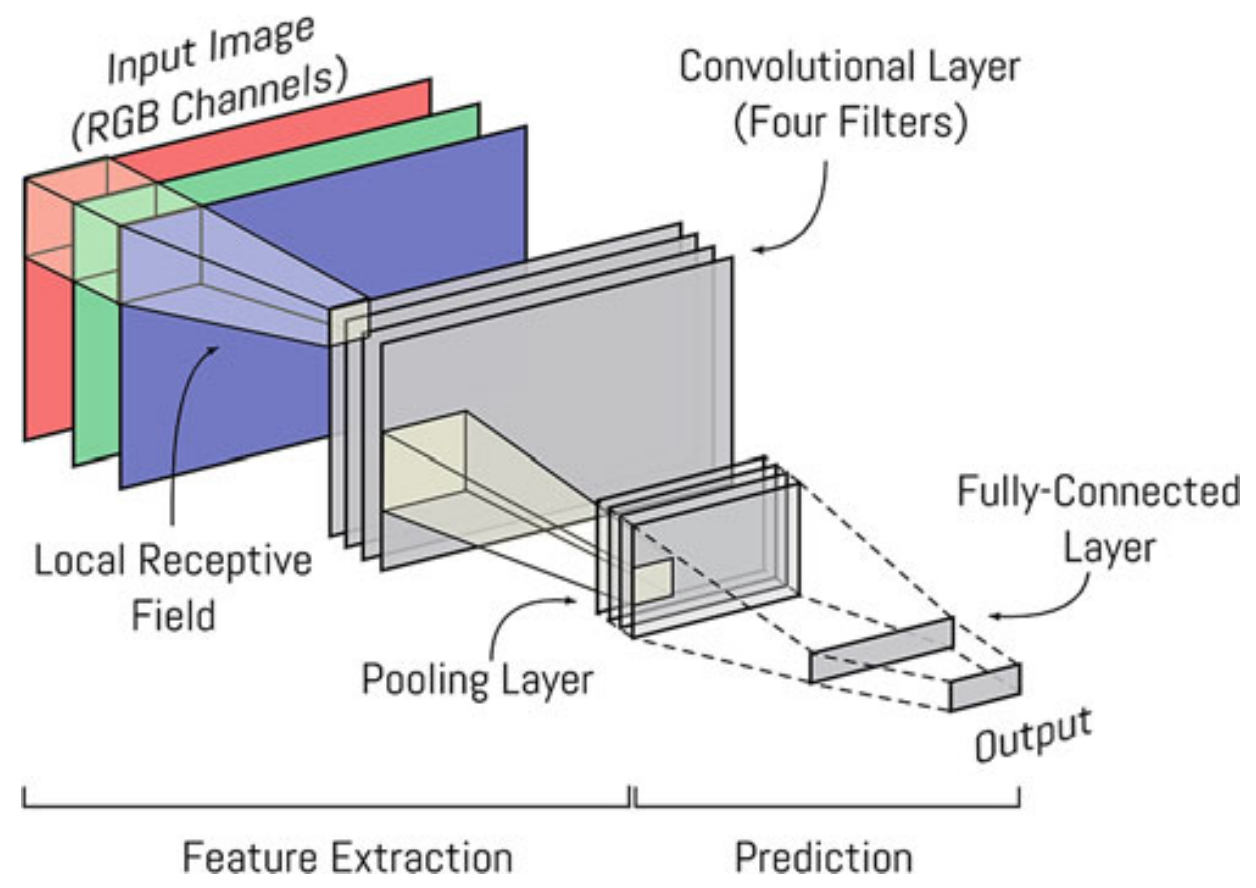
\includegraphics[scale=0.4]{backml/convnet.png}
 \caption{A \acrlong{cnn} (source \parencite{millar2019using}).}
 \label{fig:backml:cnn}
\end{figure}

Let us suppose a naive implementation of an image classifier with a \acrshort{mlp}
where each neuron in the first layer is connected to each input pixel. This model
is extremely complex and prone to overfitting, as it would realistically contain
billions of weights for a regular image. Natural images and related \acrlong{ml}
tasks have interesting properties that can be used to improve this naive model.

A first property is that \textit{pixel correlations are local}, meaning that pixels
far from each other in the image are less likely to be correlated than close
pixels. It implies that connecting individual neurons to all input pixels is
excessive and one would rather want to connect them to patches of close pixels.
A second property is that an image can be considered a \textit{stationary signal}
(\ie pixel statistics are similar at different locations of the image). Therefore,
it is relevant to use the same set of weights for all the locally-connected neurons
of a layer. These architectural choices are examples of inductive bias and motivate
the \textit{convolutional layer}. Although, we have discussed the case of images,
convolutional layers can also be generalized for 1D (\eg time series) or 3D (\eg
3D image volume) when the locality and stationarity assumptions hold.

A two-dimensional convolutional layer $h$ can be seen as a function generating an
arbitrary number $f_{out}$ of \textit{feature maps}
$\vect{a} \in \mathbb{R}^{r_{out} \times c_{out} \times f_{out}}$ from an input
$\vect{z}^{(in)} \in \mathbb{R}^{r_{in} \times c_{in} \times f_{in}}$. Feature
map $k \in \left\{1, 2, ..., f_{out}\right\}$ is the result of convoluting a
learnable weight tensor $\pmb{\theta}_k$ of dimensions $r_f \times c_f \times f_{in}$
called \textit{kernel} or \textit{filter} over the input $\vect{z}^{(in)}$:

\begin{equation}
\label{eqn:backml:convnet}
a_{ijk} = \theta_{0;k} + \sum_{s=1}^{r_f} \sum_{t=1}^{c_f} \sum_{u=1}^{f_{in}} \theta^{(l)}_{s,t,u;k} \times z^{(l-1)}_{i+s,j+t,u}
\end{equation}

where $(i, j)$ are the coordinates of a vector of $\vect{z}^{(in)}$, $\theta_{0;k}$
is the bias and $\theta^{(l)}_{s,t,u;k}$ is the weight at coordinates $(s,t,u)$
of tensor $\pmb{\theta}_k$. Similarly as for the perceptron, this linear operation
is then followed by a non-linearity:

\begin{equation}
\label{eqn:backml:convnetwithactiv}
\vect{z}^{(out)} = h\left(\vect{z}^{(in)}\right) = \sigma\left(\vect{a}\right)
\end{equation}

Convolutional layers have many hyperparameters including the number of feature
maps $f_{out}$ and filter dimensions $r_f$ and $c_f$ (typically $r_f \times c_f = 3 \times 3$
or $5 \times 5$) which both directly control the number of learnable parameters
of the layer (and therefore its complexity). In addition to those, the \textit{stride}
$s$ allows reducing the amount of computations of the layer by evaluating the
kernel every $s$ pixels (instead of every pixels) along a dimension. The
\textit{padding} defines how convolution behaves near the edges of the image where
all the considered pixels might not exist. Typical padding options are considering
missing pixels to have value 0, mirroring the image at the edge, \etc. Padding
and stride are illustrated in Figure \ref{fig:backml:paddingstride}.

\begin{figure}
  \centering
  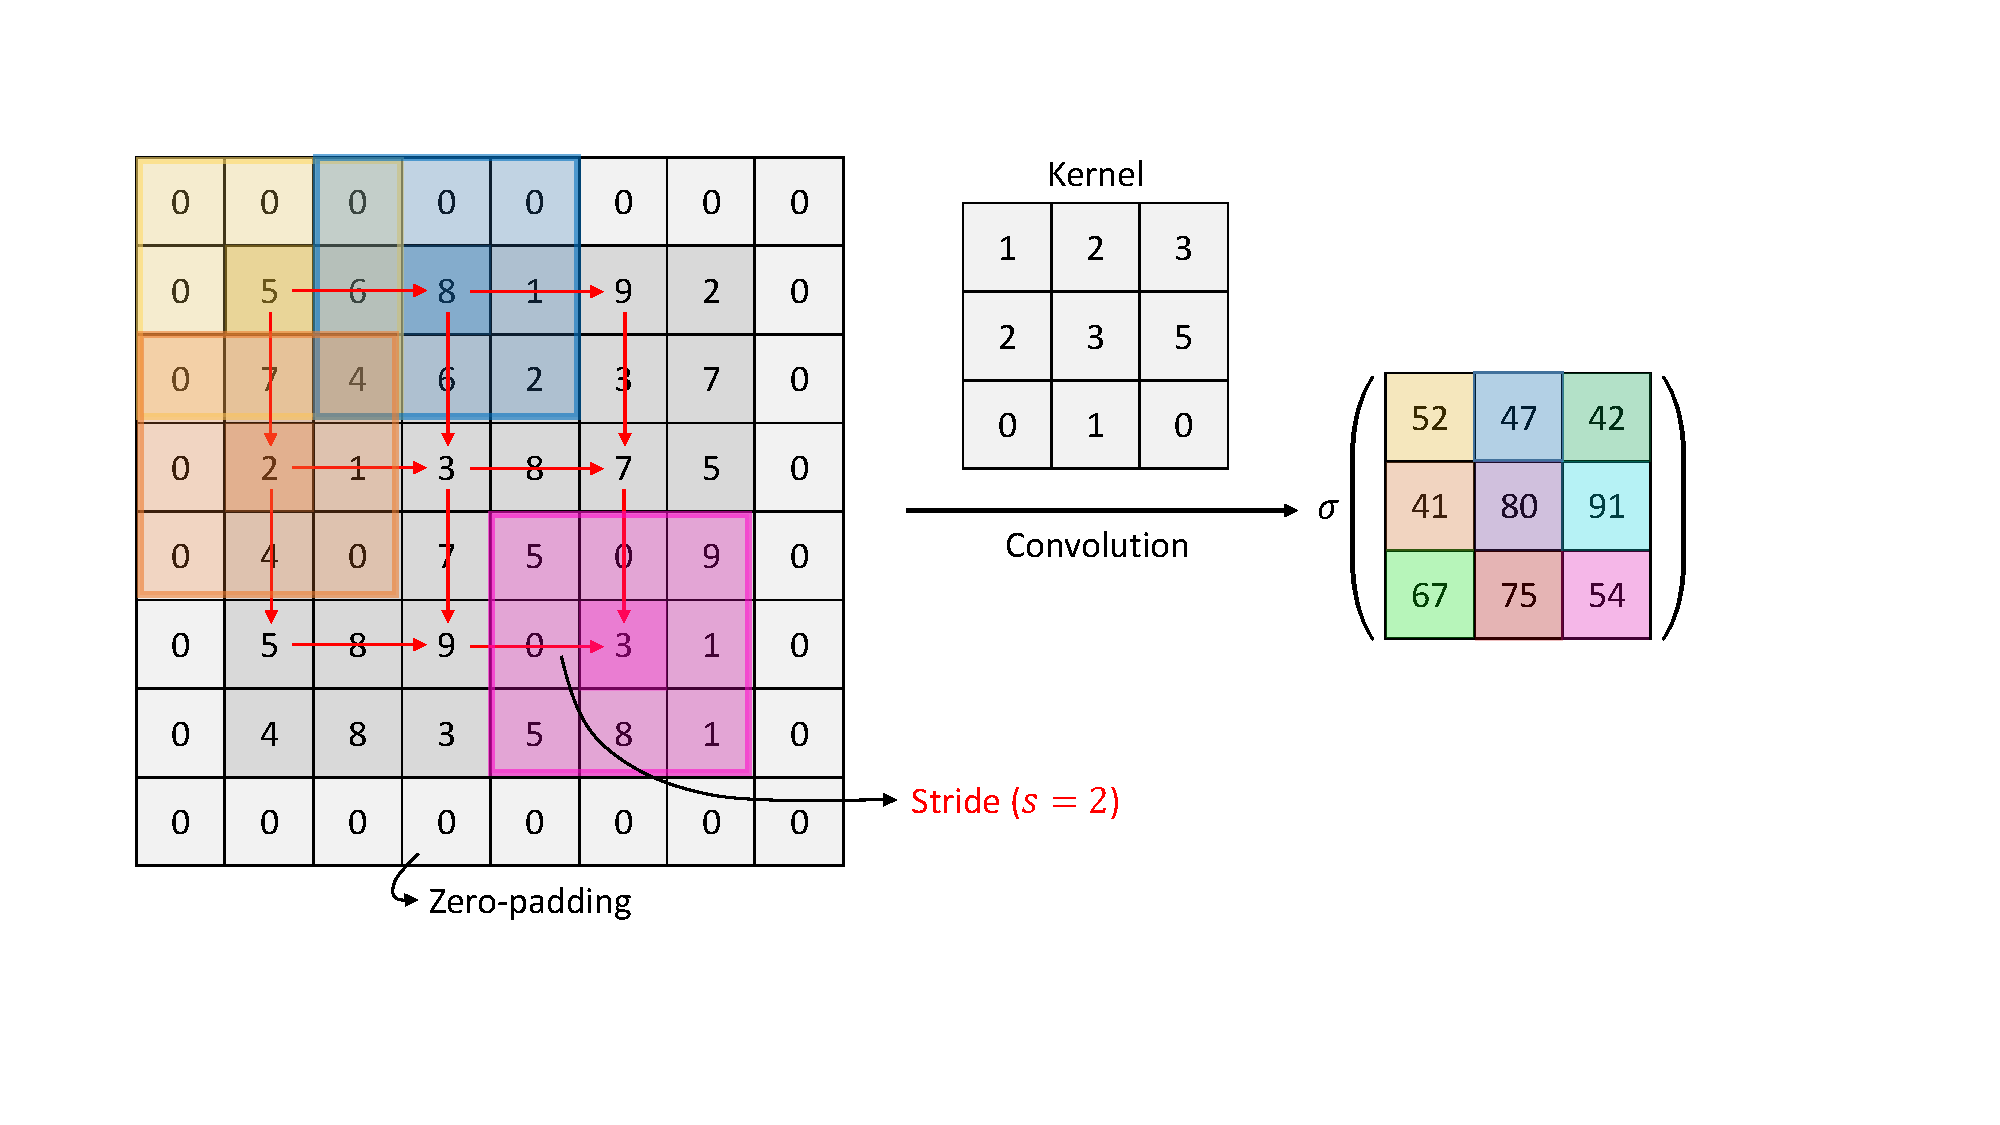
\includegraphics[scale=0.8]{backml/convolutionwithstride.pdf}
  \caption{Illustration of stride and padding.}
  \label{fig:backml:paddingstride}
\end{figure}

In addition to exploiting locality and stationarity, \acrshort{cnn}s have other
interesting properties which contribute to their efficiency for processing structured
data. They have \textit{equivariance to translation} which means that translating
the convolutional layer input along some of the dimensions only translates the
output along the same dimensions. For tasks like image classification, object
location is often irrelevant for inferring the class. Therefore, the network does
not have to learn this invariance which makes training easier. It has also been
shown that, for image classification, the learned kernels are similar to classical
computer vision filters capturing edges or color patterns in early layers and, as
one ascends the network, kernels show compositionability, invariance and class
discrimination \parencite{zeiler2014visualizing} confirming the ability of such
a network to learn and use the inherent hierarchical structure of the data. Stacking
convolutional layers also brings the benefit of increasing the receptive field of
late layers. The receptive field of an activation $a^{(l)}_{ijk}$ in a feature
map $k$ at layer $l$ is the set of pixels of the input that influence this
activation. The larger the receptive field, the more context is considered by the
activation.

\subsubsection{Pooling layer}
\label{sssec:backml:poolinglayer}

Pooling layers are another common components of \acrshort{cnn}s. Their role is to
reduce the dimensionality of feature maps by aggregating close activations. In a
way, pooling layer can be seen as a special convolutional layer with stride of
which the kernel is not learned but rather computes a possibly non-linear statistics.
The depth of the feature maps before and after pooling does not change (\ie
$f_{in} = f_{out}$). Pooling share some hyperparameters with convolution including
stride and padding. Regarding the the aggregation function, the most common choices
are \textit{max pooling} or \textit{average pooling}. The former will output the
largest activation among the one covered by the kernel:
\begin{equation}
\label{eqn:backml:maxpooling}
a_{ijk} = \text{max} \left\{ x_{i+s,j+t,k} \mid s = 1, ..., r_f; t = 1, ..., c_f \right\}
\end{equation}
The latter will average the activations covered by the kernel:
\begin{equation}
\label{eqn:backml:avgpooling}
a_{ijk} = \frac{1}{r_f \times c_f} \sum_{s=1}^{r_f} \sum_{t=1}^{c_f}  x_{i+s,j+t,k}
\end{equation}

Pooling, similarly to convolution, brings equivariance to translation and increase
the receptive field of deeper layers. The reduction of dimensionality also reduces
the computational cost of the network as deeper layers have smaller feature maps
to process. There exists other type of pooling layers which are described in
\parencite{gholamalinezhad2020pooling}.

\subsection{Neural network optimization}
\label{ssec:backml:dl:opti}
Remains the question of how to find the best parameters for the neural network
$h(\cdot; \theta)$ using a training set. Obviously, these weights should be tuned
so that the final model minimizes the expected risk (\ie the generalization error)
which is not directly possible as explained in Section \ref{ssec:backml:modelselection}.
Following the \acrshort{erm} principle, $h(\cdot; \theta)$ can be optimized by
minimizing its error on the training set measured by a loss $\mathcal{L}$. In most
cases, it is not possible to find the solution analytically and, therefore, one
resorts to numerical optimization and variants of \textit{gradient descent}
algorithms.

Starting from initial model parameters $\theta_0$, gradient descent is an algorithm
that iteratively builds a sequence of parameters $\theta_i$ such that the loss
should ideally decrease when $i$ increases. Every iteration, the parameters are
updated by applying them a correction in opposite direction of the gradients of
$\mathcal{L}$ in the parameters space:
\begin{equation}
\label{eqn:backml:gradientdescent}
\theta_{i} = \theta_{i-1} - \gamma \nabla \mathcal{L}(h(\cdot, \theta_{i}))
\end{equation}
where $\gamma$ is the learning rate, an hyperparameter for tuning the amplitude
of the parameters update.

Gradient descent does not guarantee convergence to a global minimum in general as
the optimization can either reach in a local minimum or diverge. The choices of
$\theta_0$ and $\gamma$ are important to avoid divergence. Regarding the local
minima issue, the very high-dimensional nature of neural networks makes it unlikely
to have no dimension along which the model can improve at a given iteration.
Moreover, finding parameters that achieve the global minimum of the training loss
is generally unwanted as it might lead to overfitting.

At every iteration, the original gradient descent algorithm computes gradients
over the whole training set which is particularily inefficient when $n \gg$. A
way of improving this consists in using \acrfirstit{sgd} where the gradients are
approximated using subset $\mathcal{B}$ of training samples called a \textit{batch}
instead of the whole set. This approach has been shown to be particularily efficient
for both generalization of the model and computational cost of training
\parencite{bottou201113}. When $1 < |\mathcal{B}| < n$, \acrshort{sgd} becomes
\textit{mini-batch gradient descent} which is the most used optimization strategy
for training neural networks nowadays. The batch size is often chosen based on
practical considerations like the amount of memory available on the hardware
running the learning algorithm.

Several adjustements to the gradient descent formulation of Equation
\ref{eqn:backml:gradientdescent} have shown to be effective for convergence and
stability of the optimization. In the thesis, whenever we optimize a neural network
by gradient descent, we use the Adam optimizer \parencite{kingma2014adam} approach
which normalizes the gradients using moving estimates of their mean and uncentered
variance. This method is efficient and does not require much tuning of the
hyperparameters yet makes training more robust.

\subsubsection{Backward propagation}
\label{sssec:backml:backprop}

Gradient descent, as its name suggests, heavily relies on gradient of parameters
for updating the model. The success of deep learning can be partly attributed to
an efficient algorithm for computing these gradients called \textit{backward propagation}
\parencite{rumelhart1986learning} (\aka backpropagation). The algorithm is based
on the \textit{chain rule} which states that the derivative of a composition of
functions $y(x) = (h^{(1)} \circ h^{(2)} \circ ... \circ h^{(L)})(x)$ with respect
to its input can be broken down into a product of derivatives. Given
$y_i = (h^{(1)} \circ h^{(2)} \circ ... \circ h^{(i)})(x)$, the composition of
the $i^{\text{th}}$ first functions ($i = 1, ..., L$), the chain rule states
that:

\begin{equation}
\label{eqn:backml:chainrule}
\nabla h = \dfrac{\partial h(x)}{\partial x} = \dfrac{\partial y_L}{\partial x} = \dfrac{\partial y_L}{\partial y_{L-1}} \times ... \times \dfrac{\partial y_2}{\partial y_1} \times \dfrac{\partial y_1}{\partial x}
\end{equation}

This applies directly to feedforward neural networks which are compositions of
functions and implies that computing the parameters gradients can be broken down
into computing local gradients at every layer. The backward propagation algorithm
starts from the loss and iteratively evaluates local gradients going backward in
the network until all parameters have been reached. These local gradients can then
be combined using the chain rule and the resulting gradients can be used to update
the parameters as dictated by gradient descent. This obviously requires that all
functions $h^{(l)}$ are differentiable as introduced in Section
\ref{ssec:backml:dp:components}.

Relying on gradients of a long chain of functions for the optimization can be
troublesome at times. Indeed, when a neural network is not build carefully,
\textit{vanishing} or \textit{exploding gradients} can appear. Some activations
function such as the hyperbolic tangent or the sigmoid have saturating modes as
they converge to constant values. As these fonctions converge towards a constant,
their derivatives become smaller and smaller and converge to zero. Because of the
multiplicative nature of the chain rule, one gradient in the chain is enough to
cancel all gradients upstream which happens when the activations start working in
their saturating regime. There exists best practices to reduce the likelihood of
vanishing gradients: weights must be carefully initialized, it is better to avoid
activation functions with saturating modes (\acrshort{relu} is a good candidate)
and some architectural tricks can help (see Sections \ref{sssec:backml:batchnorm}
and \ref{sssec:backml:arch:residual}). In opposition, exploding gradients cause
divergence because gradients are too large. Again architectural tricks, careful
weigths and learning rate initilization makes this issue less likely to occur.

Nowadays, all deep learning frameworks implement backward propagation and also
feature automatic differentiation. Automatic differentiation means that every
basic mathematical function present in the library is associated with its analytical
derivative. Therefore, during backpropagation, the algorithm can compute the
gradients automatically and exactly based on this information. The combination of
these two features makes training a neural network particularily easy as everything
is automated.

\subsubsection{Batch normalization}
\label{sssec:backml:batchnorm}

The \acrfirstit{bn} \parencite{ioffe2015batch} layer is part of the family of
normalization layers. This layer acts as a regularizer and is usually placed before
activations in neural networks. Given a signal
$\vect{x} = \left(\vect{x}_1, \vect{x}_2, ..., \vect{x}_f\right) \in \mathbb{R}^f$
(\eg the output of a convolutional layer), the \acrshort{bn} layer maintains an
estimate of the mean $\mu_i$ and variance $\sigma_i$ ($i = 1, ..., f$) of the
preceeding layer output computed over the batch. These estimates are used to
normalize the inputs into an intermediate signal $\hat{\vect{x}}$. Obviously,
whether this normalization is actually beneficial for the network is task-, layer-
and feature-dependent and there are probably scenarii where normalizing would hurt
performance. Therefore, the signal $\hat{\vect{x}}$ is then followed by a learnable
linear layer allowing the network to learn to revert this normalization if
necessary:

\begin{equation}
\label{eqn:backml:bn}
\acrshort{bn}(\vect{x}) = \begin{bmatrix}
\alpha_1 \left(\dfrac{\vect{x}_1 - \mu_1}{\sqrt{\sigma^2_1 + \epsilon}}\right) + \beta_1 & ... & \alpha_f \left(\dfrac{\vect{x}_f - \mu_f}{\sqrt{\sigma^2_f + \epsilon}}\right) + \beta_f \\
\end{bmatrix}\end{equation}

where the $\alpha_i$ and $\beta_i$ are the learnable parameters. During training,
the input statistics $\mu_i$ and $\sigma_i$ are computed on-the-fly using moving
averages. At inference, the statistics are frozen as well as the learnable parameters
$\alpha_i$ and $\beta_i$.

Batch normalization greatly helps network optimizition by maintaining intermediate
activations within acceptable ranges of values and therefore reducing the risk of
vanishing or exploding gradients, narrowing the parameter search and allowing
higher learning rates.

Unfortunately, the use of batch statistics can also be an issue. When there is a
sudden change in the model input distribution, the batch statistics are likely to
change quickly but the linear layer, restricted by the learning rate, will probably
not be able to adapt as quickly. This can cause instabilities while the networks
adapts its \acrlong{bn} layers for the new distribution. This situation can occur
for instance with \acrlong{tl} where source and target tasks can have drastically
different input distributions.

\TODO{explain our solution here for batchnorm in transfer issue? or section on in deep \acrlong{tl} ? or in multi task chapter?}

\subsection{Modern network architectures}
\label{ssec:backml:dl:modernarchi}

This section presents different architectures used in our contributions.

\subsubsection{Simple layer-stacking architecture}
\label{sssec:backml:arch:layerstacking}
After the success of AlexNet, researchers investigated the effect of model depth
on classification performance. An architecture in particular caught the attention
by ending up a runner up for a later edition of \acrshort{ilsvrc} in 2014. This
architecture is named VGG \parencite{simonyan2014very} after the team who participated
the challenge. It has two implementations we use in this thesis: VGG16 and VGG19.
The number is the count of layers with trainable weights in the architecture.
These architectures are pretty straightfoward (see Figure \ref{fig:backml:vgg})
as they only stack blocks of few convolutional layers with \acrshort{relu} activation
followed by pooling. The last convolutional layer is followed by a 3-layers
\acrshort{mlp}.

\begin{figure}
  \centering
  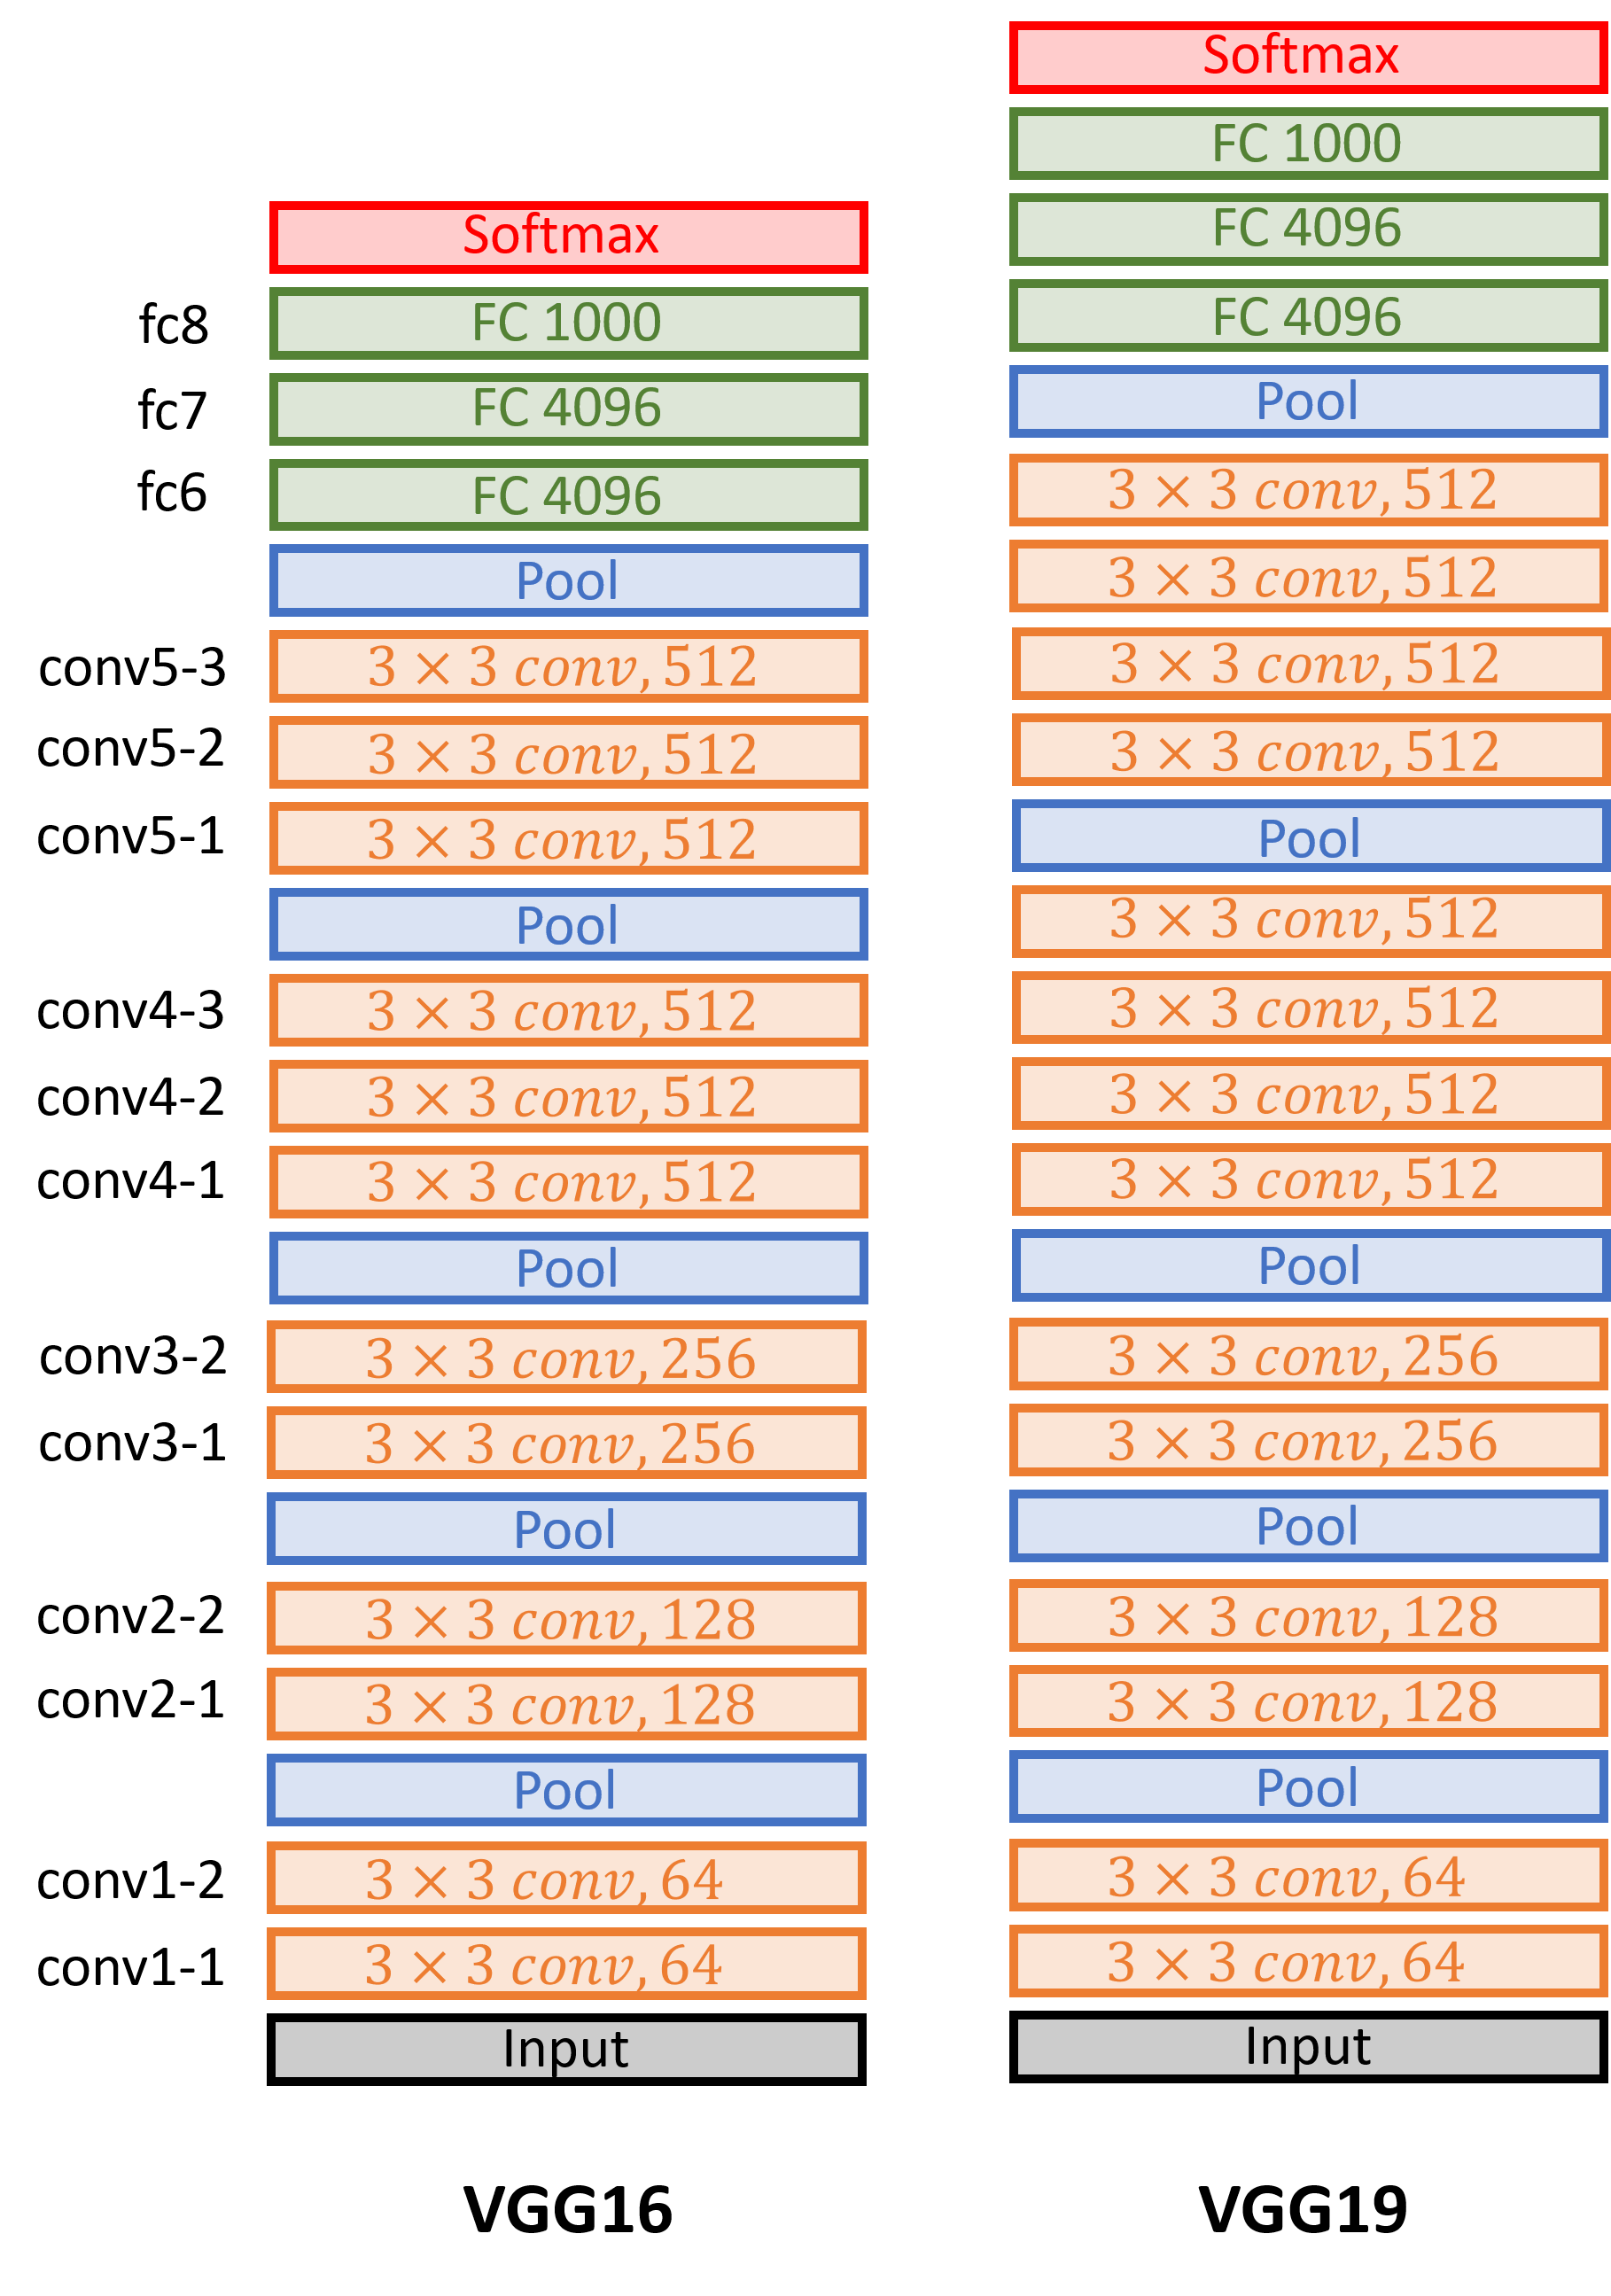
\includegraphics[rotate=-90, scale=0.28]{backml/vgg1619.png}
  \caption{VGG16 and VGG19 architectures (image from \parencite{img:vgg1619})}
  \label{fig:backml:vgg}
\end{figure}

\subsubsection{Residual architecture}
\label{sssec:backml:arch:residual}

Although improving over AlexNet, very deep networks like VGGs are subject to
training difficulties: beyond a certain model depth, accuracies sometimes start
to decrease. This can be attributed to the fact that, for a given task, adding
layers beyond a certain depth is not necessary. Moreover, it can be difficult for
gradients to flow back given the depth of the architecture (\ie vanishing gradients).
In order to address those two issues, ResNet \parencite{he2016deep} introduces
the \textit{residual mapping}, or \textit{skip-connection}. Given a layer
$h^{(l)}(\vect{x})$, the residual mapping $r^{(l)}(\vect{x})$ would be:

\begin{equation}
\label{eqn:backml:residual}
r^{(l)}(\vect{x}) = \vect{x} + h^{(l)}(\vect{x})
\end{equation}

This residual mapping makes it easier for the optimizer to simply ignore the layer
as it just has to tune all the weights in $h^{(l)}(\vect{x})$ to 0 in which case
$r^{(l)}(\vect{x}) = \vect{x}$. Moreover, gradients are still able to flow freely
through the skip-connection. This increased trainability has been empirically
confirmed as very deep residual network (up to 150 layers) have won \acrshort{ilsvrc}
in 2015 and 2016 and have shown impressive performance in many other contexts.
Another advantage of residual networks is that, even though they are deeper than
their VGG counterparts, they need much less parameters to reach better
performance\footnote{VGG16 and 19 have more than 140M parameters whereas ResNet50 has 25M and the largest ResNet152 has 66M parameters.}
making ResNets more lightweight. Nowadays, residual connections are a common
building block in deep architectures. In this thesis, we use one of the first
iteration of ResNets, namely ResNet50 (see Figure \ref{fig:backml:resnet} for
ResNet34, a similar architecture).

\begin{figure}
  \centering
  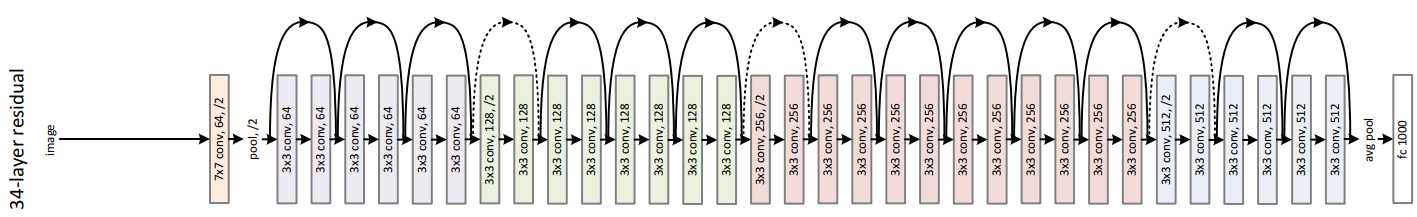
\includegraphics[scale=0.4]{backml/resnet34.png}
  \caption{ResNet34, same design as ResNet50 but less layers. Residual connections are placed every two convolutional layers (image from \parencite{he2016deep}).}
  \label{fig:backml:resnet}
\end{figure}

\subsubsection{Inception architecture}
\label{sssec:backml:arch:inception}
% InceptionV3
% InceptionResNetV2
The winning method of \acrshort{ilsvrc}2014 was based on an architecture called
GoogLeNet \parencite{szegedy2015going} (\aka InceptionV1). This architecture is
based on \textit{inception modules}. An inception module is a composition of
convolutional layers built to maintain a certain level representativeness while
reducing the number of training parameters compared to a block of plain convolutional
layers. An example of a trick used to reduce the number of parameters is to use
two consecutive $3 \times 3$ instead of one $5 \times 5$ convolutional layers. In
this thesis, we use InceptionV3 \parencite{szegedy2016rethinking}, the third
iteration of the architecture, which essentially scales it up by using factorized
convolutions and regularization. We also use InceptionResNetV2, a version of the
Inception architecture using residual connections
\parencite{szegedy2017inception}.


\subsubsection{Dense architecture}
\label{sssec:backml:arch:dense}
The densely connected convolutional networks \parencite{huang2017densely} push
further the idea of residual connection. Let us suppose a group $g$ of $L$
consecutive convolutional layers $h^{(l)}$ ($l = 1, ..., L$) taking $\vect{x}$ as
input. In this group, each layer $h^{(l)}$ receives as input the outputs of all
preceeding layers $h^{(i)}$ ($i = 1, ..., l-1$) and the input signal $\vect{x}$.
This group $g$ is called a \textit{dense block} and is the basis for the densely
connected networks. Such networks typically stack several dense blocks connected
together with one convolution and one pooling layers (see Figure
\ref{fig:backml:densenet}).

\begin{figure}
  \centering
  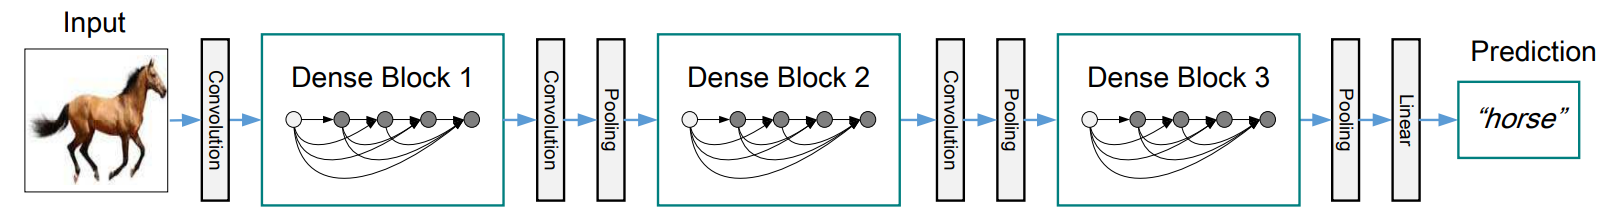
\includegraphics[scale=0.35]{backml/densenet.png}
  \caption{A densely connected network (image from \parencite{huang2017densely}).}
  \label{fig:backml:densenet}
\end{figure}

\subsubsection{A segmentation architecture, UNet}
\label{sssec:backml:arch:segment}

For tackling image segmentation tasks, one generally uses \textit{\acrlong{fcn}s}
(\acrshort{fcn}) which is a kind of network where (almost) all layers are
convolutional. One of the most popular architecture for segmentation is a U-shaped
network called U-Net \parencite{ronneberger2015unet}. This architecture is composed
of a contracting and an expanding paths (hence the ``U'', see Figure
\ref{fig:backml:unet}). Similarly as for classification networks, the former is
composed of convolutional and pooling layers that progressively encodes the input
images into high-level context features. The latter combines decoded high-level
features with low-level features from the expanding path to eventually generate
a segmentation map. The decoding of low-level features is learned using an
upconvolution layer. Upconvolution is a layer that upsamples a signal with a
learnable filter. In order to combine decoded high level features and low-level
features, U-Net uses skip connections from the contracting to the expanding
paths.

\begin{figure}
  \centering
  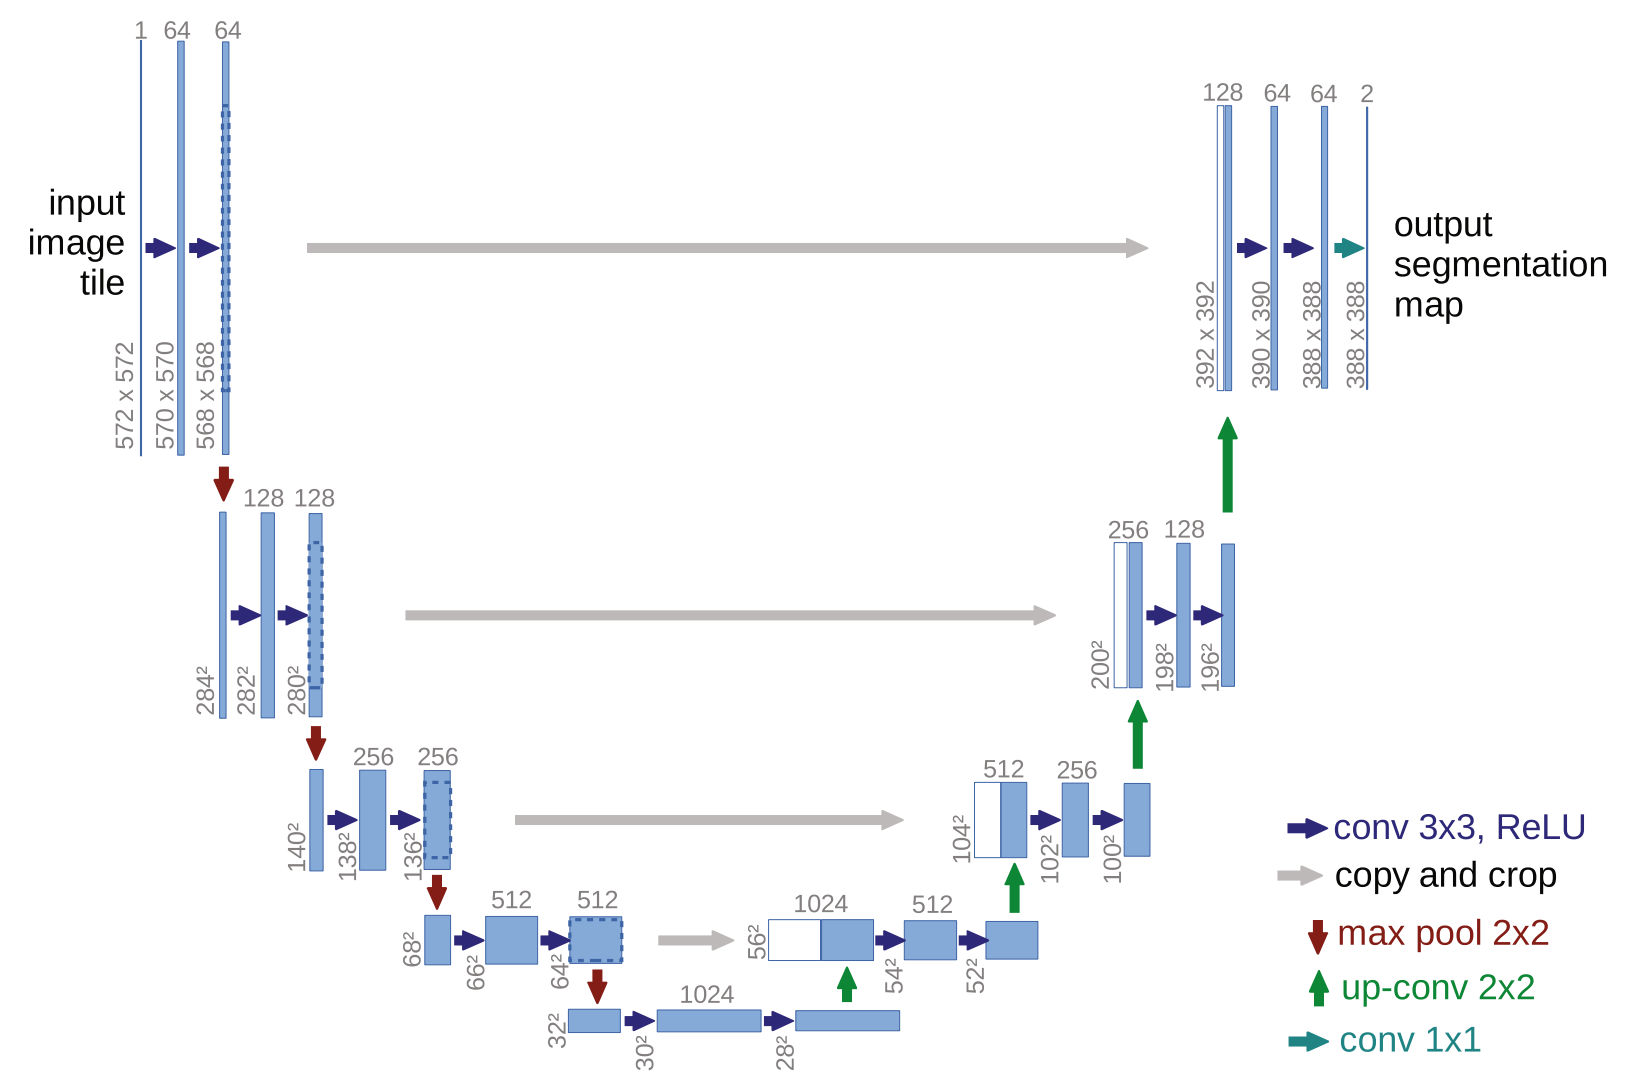
\includegraphics[scale=0.35]{backml/unet.png}
  \caption{U-Net architecture (image from \parencite{ronneberger2015unet}).}
  \label{fig:backml:unet}
\end{figure}

\subsection{Deep transfer learning}
\label{ssec:backml:dl:deeptransfer}

As presented in Section \ref{ssec:backml:transfer}, \acrlong{tl} regroup several
families of methods which have been and continue to be explored through the prism
of \acrlong{dl} \parencite{tan2018survey}. In this thesis, we focus on supervised
model-based (or network-based) \acrlong{tl} applied to image classification. With
this approach, knowledge is encoded through the parameters of a model. This model
is first trained on a source task, usually a large image classification dataset,
then transfered to the target task.

There are two approaches for transfering a deep neural network to a target task.
Let us consider three networks $h_s$, $h_o$ and $h_n$ respectively parametrized
by $\theta_s$, $\theta_o$ and $\theta_n$. In the remaininder of this section, we
will designate a network interchangeably by its set of parameters $\theta_i$ or
its function $h_i(\cdot;\theta_i)$. The network $\theta_s$ is shared between the
source and target tasks and $\theta_o$ and $\theta_n$ are the task-specific
networks. Both approaches first require the network $h = h_s \circ h_o$ to be
trained on the source task. At the end of training, $\theta_s$ encodes the knowledge
to be transfered.

\begin{figure}
  \centering
  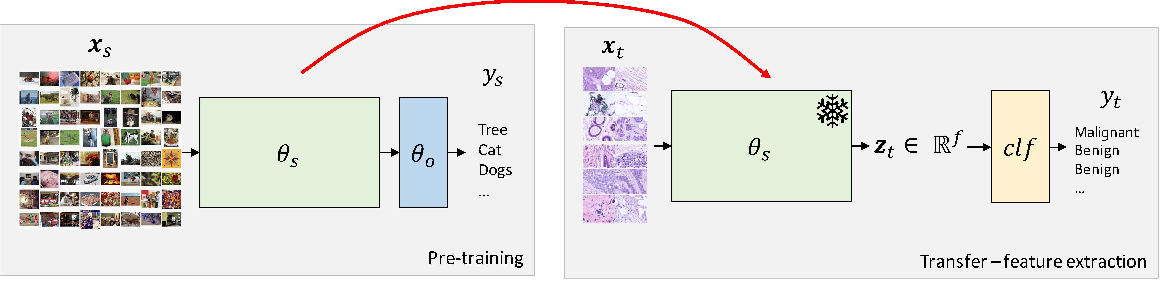
\includegraphics[scale=0.8]{backml/transfer-fe.pdf}
  \caption{Supervised \acrlong{tl} by \textit{feature extraction}. The shared network is trained by supervised learning on the source task. Then, the shared part $\theta_s$ is extracted and used as an encoder for images of the target task. A third-party classifier $clf$ can be trained and used to classify the encoded target data.}
  \label{fig:backml:transfer-fe}
\end{figure}

The first transfer approach is \textit{feature extraction} (see Figure
\ref{fig:backml:transfer-fe}) and simply consists in generating a new representation
for samples of the target task using $\theta_s$ as an encoder. For each sample
$\mathbf{x}_i$ of the target task, this encoder generates a feature vector
$\vect{z}_i = h_s(\vect{x}_i;\theta_s) \in \mathbb{R}^f$ where $f$ is the number
of features. The encoder is said to be ``\textit{frozen}'' as it is not updated
after transfer. The generated features can be used to train a third-party classifier
on the target task which can be as simple as a linear model. A common choice of
classifier is a linear \acrshort{svm}.

\begin{figure}
  \centering
  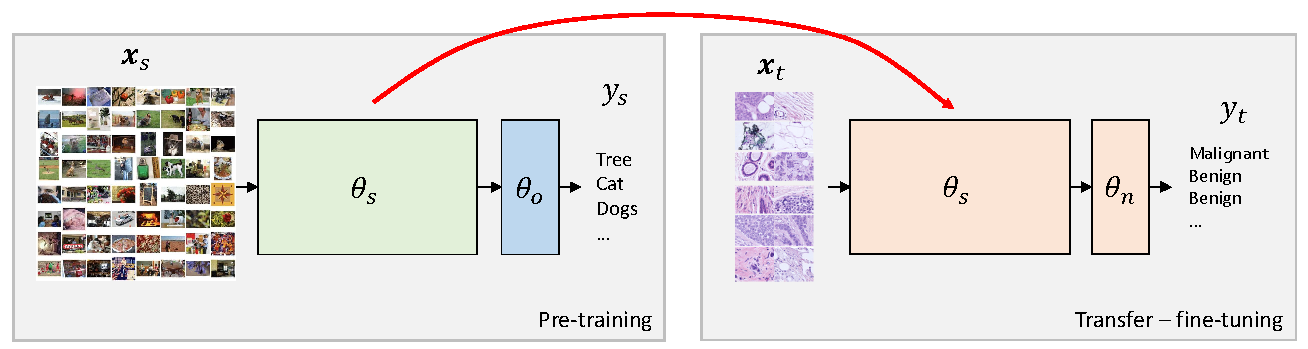
\includegraphics[scale=0.85]{backml/transfer-ft.pdf}
  \caption{Supervised \acrlong{tl} by \textit{fine-tuning}. The shared network is trained by supervised learning on the source task. Then, the shared part $\theta_s$ is extracted and attached $\theta_n$. The network $h_s \circ h_n$ is trained by gradient descent on the target task.}
  \label{fig:backml:transfer-ft}
\end{figure}

The second transfer approach is \textit{fine-tuning} (see Figure \ref{fig:backml:transfer-ft})
where the task-specific part of the network $\theta_{o}$ is replaced by a new
classification network $\theta_{n}$ and the resulting network $h = h_s \circ h_n$
is further trained by gradient descent on the target task. Subjecting the whole
network to gradient descent will change the features learned on the source task
which can cause catastrophic interference. Therefore, a way of alleviating the
issue is to use a small learning rate (compared to the initial training learning
rate). Another of way preventing this issue consists in freezing a part of
$\theta_s$, usually the first layers.

The feature extraction approach only emerged recently with works on the Overfeat
\parencite{sermanet2013overfeat, razavian2014cnn} and Decaf \parencite{donahue2014decaf}
convolutional architectures. The authors trained their AlexNet-based networks in
a supervised manner on the large ImageNet source dataset composed of 1.2 millions
natural images and 1000 distinct classes. They both showed that these networks
were able to produce discriminative features for tasks they were not trained on.

Building upon these results, \parencite{yosinski2014transferable} analyzed the
transferability of deep neural networks using both approaches in more details.
Their most prominent conclusion is that features in a neural network become less
transferable as one moves deeper in the network indicating that the network features
shift from generic to specific along the network. This result is consistent with
\parencite{zeiler2014visualizing} as early layers typically learn classical computer
vision filters. This motivates freezing only the first layers of the network to
avoid catastrophic interference as they are more generic and therefore should not
require much tuning. They also studied how task similarity impacted transfer
performance and found that similar tasks indeed benefited better from transfer
than dissimilar ones.

Whereas the versatility of ImageNet initially fueled research in deep \acrlong{tl}
with supervised model pre-training, several recent contributions have shown that
pre-training could be performed differently. For instance, SimCLR \parencite{chen2020simple}
uses contrastive learning to learn the model. This is a self-supervised approach
which consists in generating pair of similar and dissimilar images using data
augmentation and training a network to discriminate these pairs. They have shown
that the resulting network has learned discriminative features that can be transfered
quite efficiently to new tasks. The \acrfirstit{vit} \parencite{dosovitskiy2020image}
is another approach based on transformers, a recent and popular family of
attention-based methods. Attention is a mechanism of selection of information
which can be implemented in different ways in neural networks \parencite{niu2021review}.
It has initially been applied with great successes on \acrfirstit{nlp} problems
but \acrshort{vit} has shown that attention-based architectures are also applicable
to vision. In this framework, the transfer process is very similar to supervised
pre-training as the model is first trained in a supervised manner on a large
database, then transfered to the target task. The only difference is that the
attention-based network does not use convolution and takes as input a sequence of
non-overlapping patches of the image. Other contributions focus on improving
classical supervised pre-training approach. For instance, \parencite{wang2019pay}
combine \acrlong{tl} and model compression as the fine-tuning process excludes
non-informative feature maps from the final model based on their \acrfirstit{afds}
mechanism.

Because of its ability to tackle data scarcity, \acrlong{tl} has been a method of
choice in many applications where this problem occurs. In Section \ref{ssec:backdp:tl},
we explore further applications of \acrlong{tl} to \acrlong{dp} and medical imaging
in general.

\section{Wrapping up}
\label{sec:backml:wrapup}

In the previous sections, we gave an overview of different topics. We can now position our work in this context. In Chapters \ref{chap:comp}
and \ref{chap:mtask}, both contributions explore heterogeneous model-based
\acrlong{tl} by transfering \acrlong{dl} classification models. We use several
target tasks to study how \acrlong{tl} performs in the context of \acrlong{dp}
(more on this in Chapter \ref{chap:backdp}). The first contribution studies transfer
from ImageNet. Motivated by the fact that transfer works better when the source
and target tasks are related, the second contribution use homogeneous features-based
\acrlong{mtl} as a way to pre-train a model for transfer on \acrlong{dp} data
directly.

In Chapter \ref{chap:sdist}, we move to a different type of task: image segmentation.
Working with an sparsely-annotated \acrlong{dp} dataset, we use self-training to
complete the areas where annotations are missing. We train a U-Net segmentation
model on the self-annotated segmentation.

\TODO{chapter on software contributions}

\chapter{Digital pathology}
\label{chap:backdp}

\begin{overview}{Overview}
  This chapters presents an overview of digital and \acrlong{cpath} from the perspective of a computer scientist and aims at providing basic understanding of what makes \acrlong{cpath} a challenging but promising topic. Section \ref{sec:backdp:wsi} presents a typical histological glass slide preparation process, how this glass slide is transformed into an image and what could go wrong during these processes. Section \ref{sec:backdp:typicalanalysistasks} discusses briefly how slides are used and analyzed by practioners and provides three use cases where \acrlong{cpath} could greatly help pathologists in their day-to-day work. Finally, in Section \ref{sec:backdp:ml}, we present some the challenges specific to the application of machine learning to \acrlong{cpath} including data leakage and data scarcity and how to tackle them. This last section also presents the related works of our contributions.
\end{overview}

% analogintelligence.com image dp illustration

\section{What is \acrlong{dp}?}
\label{sec:backdp:whatisdp}

Nowadays, medicine and healthcare rely heavily on analysis of human body samples to study and diagnose diseases. The branch of medicine focusing on this analysis is called \textit{pathology} which includes histology-based pathology (\aka histopathology) and cytology-based pathology (\aka cytopathology). Both of these sub-branches involve the study of microscope glass slides containing samples (see Figure \ref{fig:backdp:glassslides}). Histology samples are tissue sections cut from a bodily specimen. Cytology is concerned with samples of free cells or tissue fragments.

\begin{figure}
  \centering
  \begin{subfigure}[t]{0.48\textwidth}
    \centering
    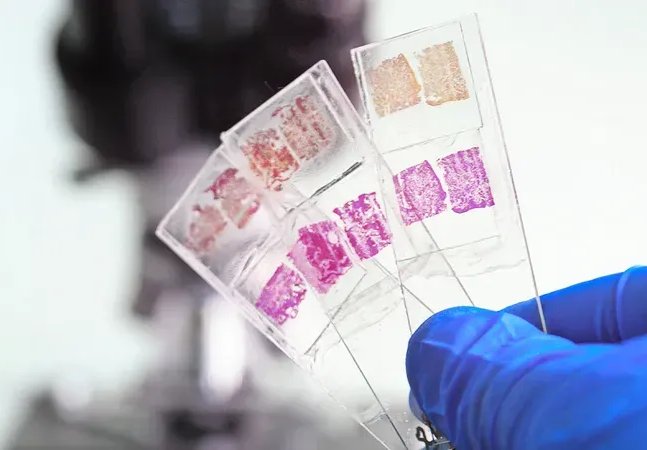
\includegraphics[height=150pt]{backdp/microscope-slide.png}
  \end{subfigure}
  \begin{subfigure}[t]{0.48\textwidth}
    \centering
    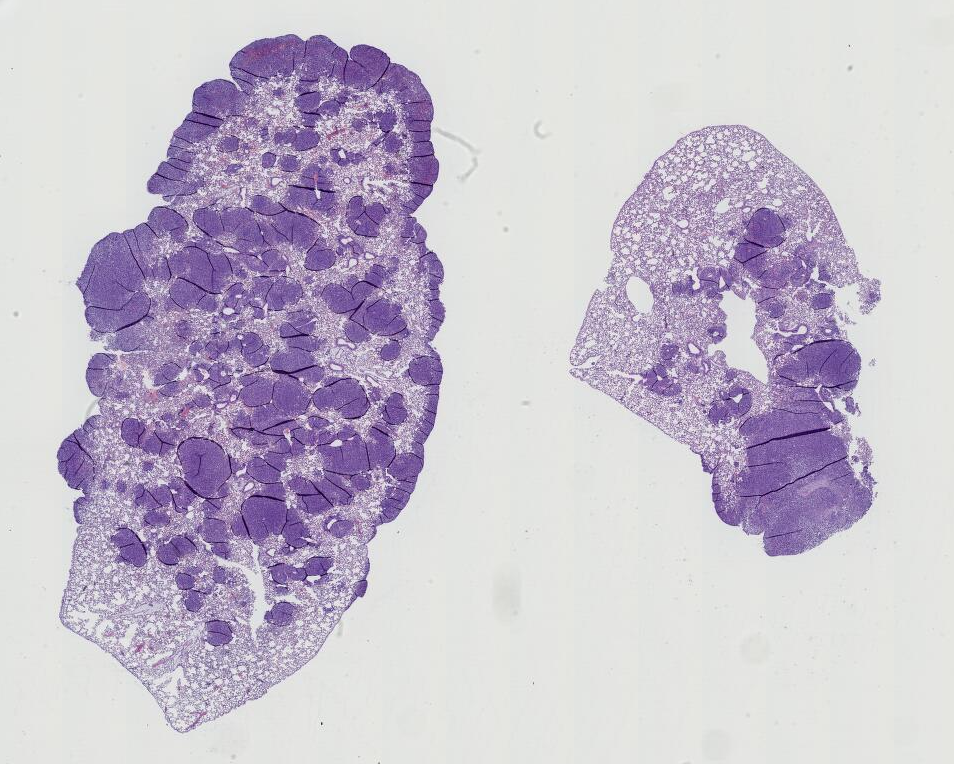
\includegraphics[height=150pt]{backdp/wsi.png}
  \end{subfigure}
  \caption{\textit{Left:} microscope slides with tissue samples (source: \parencite{img:glassslides}). \textit{Right:} a whole-slide image of dimensions 30720 x 25600 pixels}
  \label{fig:backdp:glassslides}
\end{figure}

The trend of digitalization affecting our societies also impacts pathology as, using dedicated scanners, these glass slides can now be digitized into large image files called \acrfirstit{wsi}. These files associated with subject metadata are stored in computer systems commonly called \acrfirst{pacs} or \acrfirst{lis}. In this context, \acrfirstit{dp} can be defined as ``\textit{the acquisition, management, sharing and interpretation of pathology information - including slides and data - in a digital environment}'' \parencite{doolan2019whatisdp}. Working with \acrshort{wsi} instead of physical slides has several advantages and drawbacks. Aside from easier sharing and storing of slides, digitization also opens the way for automated analysis sofware to automatically extract relevant information, typically with the help of \acrlong{ai} and \acrlong{ml}. The branch of \acrlong{dp} interested in such analysis is called \acrfirstit{cpath} and holds great promises for the future. Indeed, \acrlong{cpath} techniques have the potential to relieve pathologists from easy but time-consuming tasks allowing them to focus on challenging cases and research therefore reducing healthcare cost and improving diagnosis quality. On a larger scale, they hold promises for increased coverage and quality of healthcare around the world and especially in low incomes countries where the number of pathologists per inhabitant is typically insufficient. According to the \acrshort{who} cancer report \parencite{world2020report}, the ratio of pathologist per inhabitant was approximately 1 per 15000 in high income countries in 2020 but dramatically drops to 1 per million or less in many low income countries. A throrough list of advantages and drawbacks of \acrlong{dp} can be found in Table 1 of \parencite{jahn2020digital}.

Interestingly, although digitization technologies are quite mature, adoption of \acrlong{dp} in healthcare facilities is not simple. Many still heavily rely on glass slides for day-to-day operations. Indeed, the transformation requires to modernize the whole hardware (scanners, workstation) and software (slide viewers, information system) infrastructures and to re-think entirely the processes of the facility \parencite{temprana2022digipatics}. This obviously requires significant investments both in time and money and careful planning to carry it out successfully which is not always comptabile with the workload of pathology services or research laboratories. Other difficulties might arise, slowing down the transformation, such as reluctance to change and lack of confidence in modern tools for slide visualization and analysis. 
%Moreover, some tasks cannot be performed easily on \acrlong{wsi}s but can on a glass slide (\eg exploring the depth of a sample in cytology by changing the focal plane). 

As far as automated analysis is concerned, it remains quite a challenge. Whole-slide images typically contain several billions of pixels at full resolution which implies longer processing times and memory issues compared to classical images. Moreover, for most tasks, the image content is complex and traditional computer vision methods (\eg thresholding) would often fail to distinguish structures of interest. This complexity is increased by the presence of artifacts \parencite{taqi2018review} appearing during the conversion process of a bodily specimen to an image. An artifact is a visual or physical alteration of a sample that can hamper its analysis, automated or not. Artifacts introduce a source of variability that algorithms must learn to deal with. At worst, they can prevent any meaningful analysis by hiding, destroying or changing the appearance of the structures of interest (more on artifacts in Section \ref{sec:backdp:wsi}). The ability of learning techniques to train models that capture complex relationships in data makes \acrlong{ml} an ideal candidate to tackle \acrlong{cpath} tasks. However, data scarcity is a prevalent issue in the field as quality data, especially annotated, can be difficult to obtain for various reasons: privacy concerns, time-consuming and expensive nature of the annotation process, \etc.     

Overall, \acrlong{dp} holds great promises but presents significant and interesting challenges on several fronts. This thesis focuses on the \acrshort{ml}-based automated analysis aspects of \acrlong{cpath} and studies how to tackle data scarcity in particular.

\section{A journey from the body to the computer}
\label{sec:backdp:wsi}

Turning a bodily specimen into \acrlong{wsi}s is a long and complex multi-step process typically involving the work of several highly-specialized technicians and machines. Some steps can nowadays be automated but the chain remains mostly manual. In this section, we describe the different steps of this procedure which is summarized in Figure \ref{fig:backdp:overallprocess}. An alternate presentation of the process can be found in \parencite{mccann2014automated} (including illustrations). Sample preparation can differ more or less dependending on the nature of the sample (\eg histology, cytology, hematology) or target imaging technique (\eg brightfield, fluoresence, multispectral). For the sake of brevity, our description focuses on histology with a tissue section prepared for brightfield microscopy and scanning, brightfield being one of the most common modalities used in histo- and cytopathology. We will also present a few technical details related to \acrshort{wsi} files structure and visualization. 

Throughout the section, we will discuss some of the possible artifacts resulting from the transformation procedure. Our presentation of artifacts will not be exhaustive and few visual examples can be found in Figure \ref{fig:backdp:artifacts:all}. A more thorough list of pre-scan artifacts with illustrations can be found in \parencite{taqi2018review}.

\begin{figure}
  \centering
  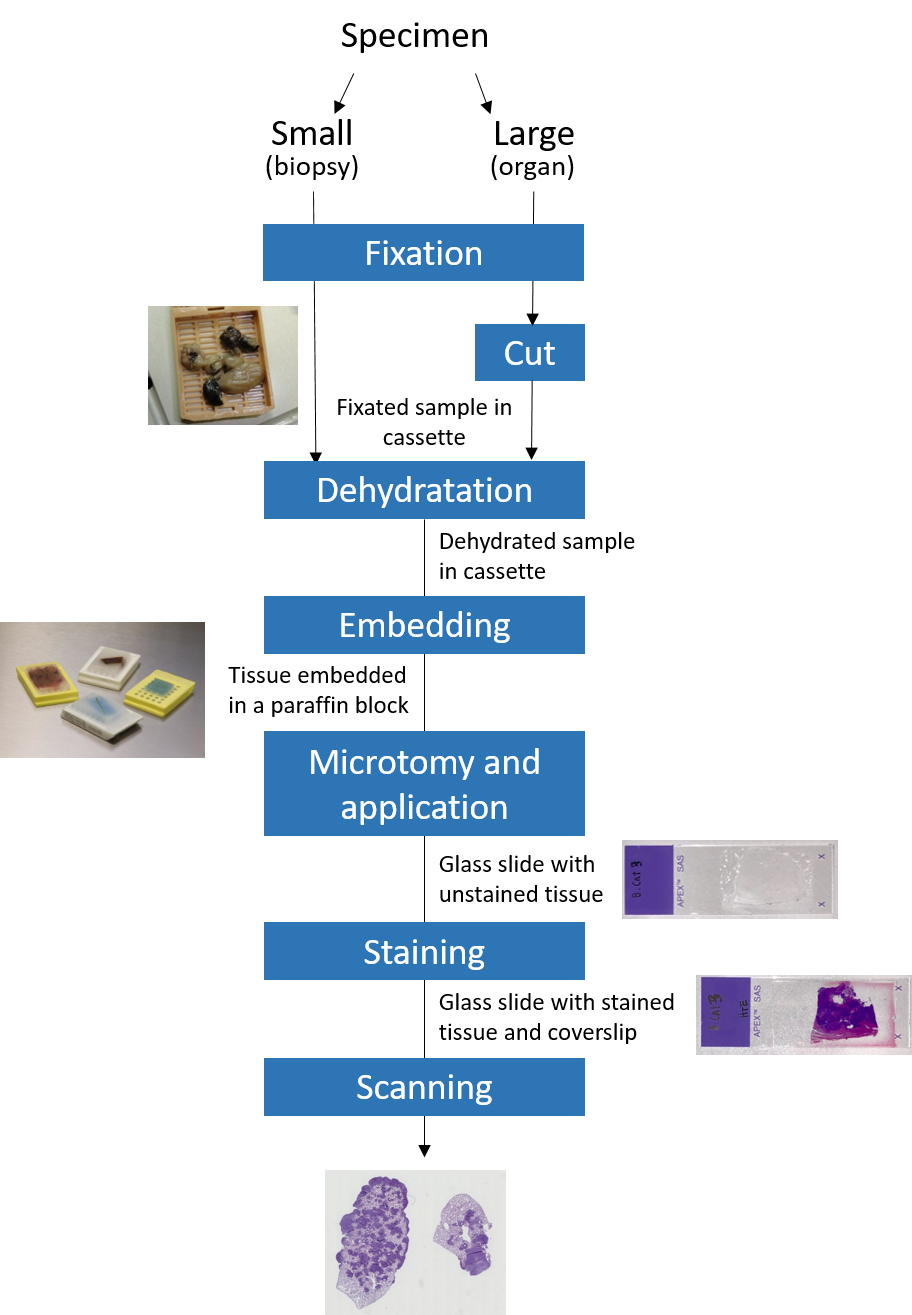
\includegraphics{backdp/overallprocess.png}
  \caption{Summary of the transformation of a specimen into a \acrlong{wsi}.}
  \label{fig:backdp:overallprocess}
\end{figure}

\subsection{Specimens collection, fixation, cutting and dehydratation}

Whether it is for research or diagnosis, the slide preparation process starts with a specimen, a piece of human or animal body for which a question must be answered. The specimen can be as large as a whole organ but can also be as small as a drop of bodily material commonly referred to as a \textit{biopsy}. Before going through the preparation process, a specimen must be fixated. The goal of fixation is to put a stop to the natural decay of the specimen and increase its structural stability \parencite{rolls2012process}. This can be achieved, for instance, by immersing the specimen in a formaldehyde bath (\ie the fixative solution) for period of time depending on its size (\ie few hours to a whole day). 

When the specimen has been fixated, it is then placed into a standardized container called a \textit{cassette} (see Figure \ref{fig:backdp:cassette}). If it is too large for the cassette (\eg an organ), one or more volumes of interest are cut from the specimen. Depending on the later examination, the orientation of the cut can be crucial to exhibit relevant tissue structures of the specimen. In the remaininder, we will call a \textit{sample} the content of this cassette.

For a proper analysis, the tissue morphology of the sample must be preserved. This is most commonly achieved by infiltrating the tissue with paraffin wax. Infiltration however does not work on a raw fixated tissue because paraffin is hydrophobic. Therefore, one must first perform \textit{dehydratation}, that is, replacing water naturally present in the sample with a product miscible with paraffin. This is done by first immersing the sample into a succession of alcoholic solution baths. Although this process achieves dehydratation, alcohol does not mix with paraffin neither. Therefore, the sample is then immersed into one or more xylene-based solutions baths, xylene being miscible with both alcohol and paraffin. The sample, infiltrated with xylene, is finally immersed in a paraffin bath under vacuum. The dehydratation process takes few hours and is often automated using dedicated machines.

The earliest source of artifacts is the specimen extraction process itself. The specimen can indeed be damaged by the use of certain tools (\eg burned by an electrical scalpel) or treatment at the extraction site. Unlike these, the following artifacts are caused by the early stages of the slide preparation process. Bad fixation can lead to decaying tissue (\ie autolysis) and structural degradation (\eg tissue shrinkage). Improper cutting can also cause tissue damage like tearing and squeezing. Improper dehydratation can leave some parts of the sample with remaining water, alcohol or xylene. Tissues can also be exposed to the different solutions for an excessive duration. These processing errors can for instance cause tearing, shrinkage, interference with the staining process (see Section \ref{ssec:backdp:staining}) and affect the structural properties of the tissue (\eg tissue becomes brittle).

\begin{figure}
  \centering
  \begin{subfigure}[t]{0.32\textwidth}
    \centering
    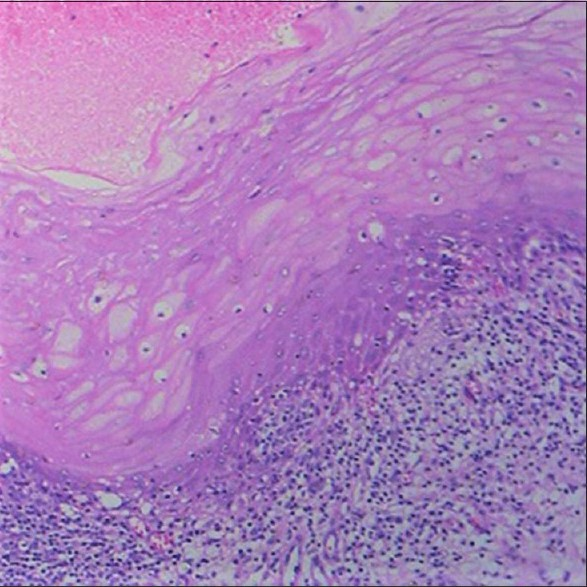
\includegraphics[width=0.98\textwidth]{backdp/JOMFP-22-279a-g007_square.jpg}
    \caption{}
    \label{fig:backdp:artifacts:autolysis1}
  \end{subfigure}%
  \begin{subfigure}[t]{0.32\textwidth}
    \centering
    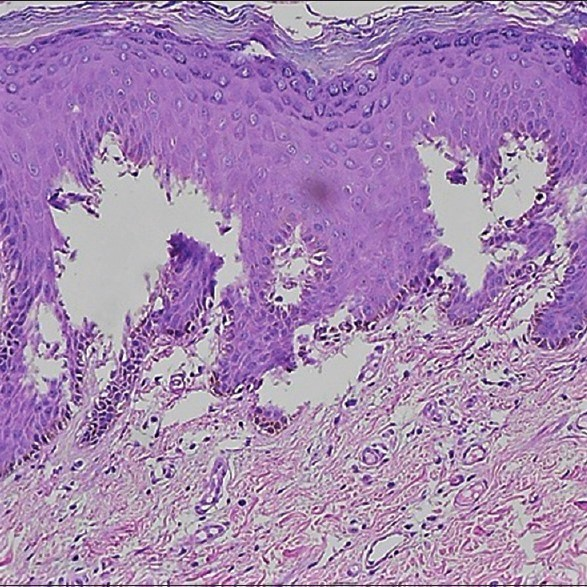
\includegraphics[width=0.98\textwidth]{backdp/JOMFP-22-279a-g008_square.jpg}
    \caption{}
    \label{fig:backdp:artifacts:autolysis2}
  \end{subfigure}%
  \begin{subfigure}[t]{0.32\textwidth}
    \centering
    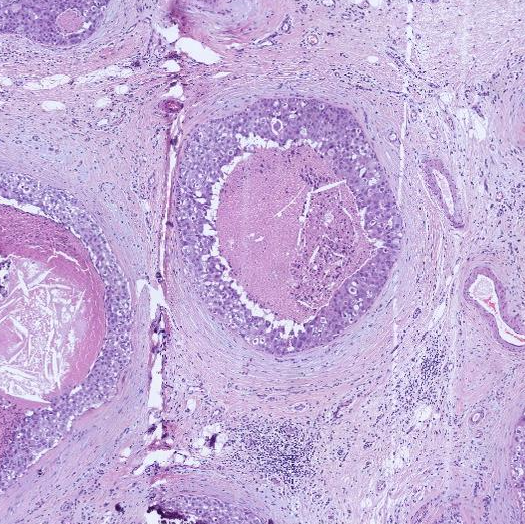
\includegraphics[width=0.98\textwidth]{backdp/artifact_dull_blade.png}
    \caption{}
    \label{fig:backdp:artifacts:microtomy1}
  \end{subfigure}\\

  \begin{subfigure}[t]{0.32\textwidth}
    \centering
    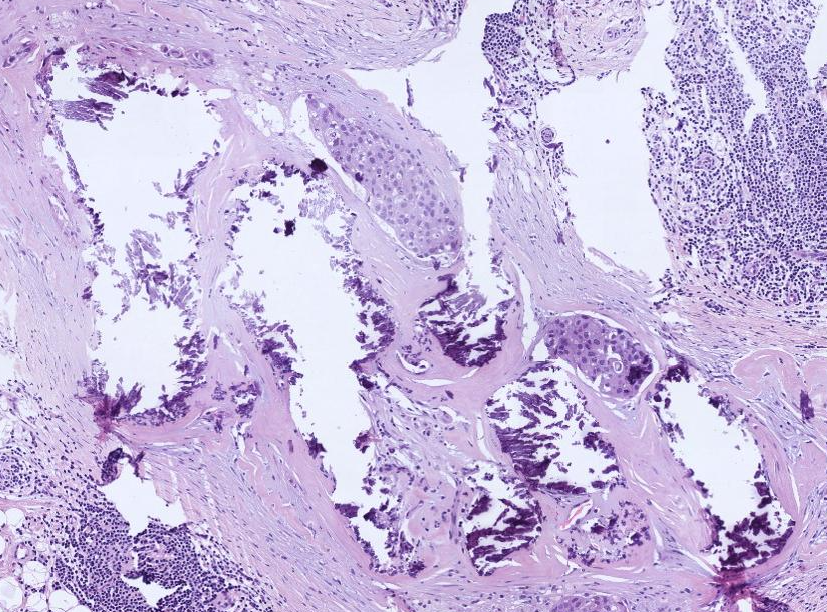
\includegraphics[width=0.98\textwidth]{backdp/calcification.png}
    \caption{}
    \label{fig:backdp:artifacts:microtomy2}
  \end{subfigure}%
  \begin{subfigure}[t]{0.32\textwidth}
    \centering
    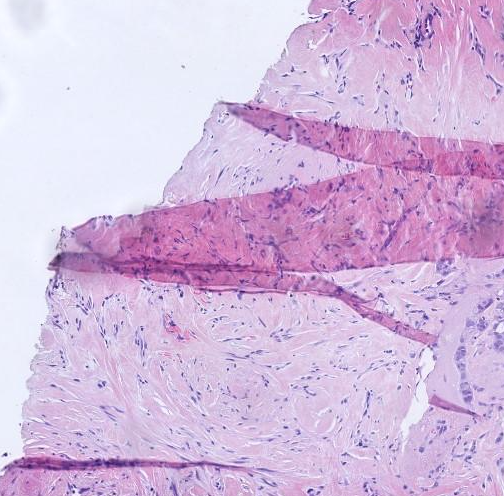
\includegraphics[width=0.98\textwidth]{backdp/folding_artifact.png}
    \caption{}
    \label{fig:backdp:artifacts:folding}
  \end{subfigure}%
  \begin{subfigure}[t]{0.32\textwidth}
    \centering
    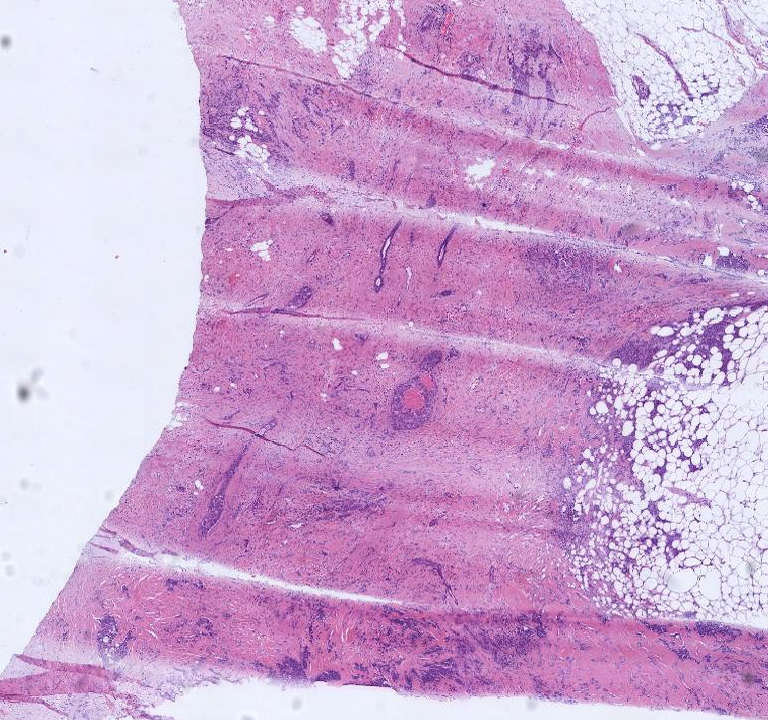
\includegraphics[width=0.98\textwidth]{backdp/staining_artifact.png}
    \caption{}
    \label{fig:backdp:artifacts:staining}
  \end{subfigure}\\

  \begin{subfigure}[t]{0.32\textwidth}
    \centering
    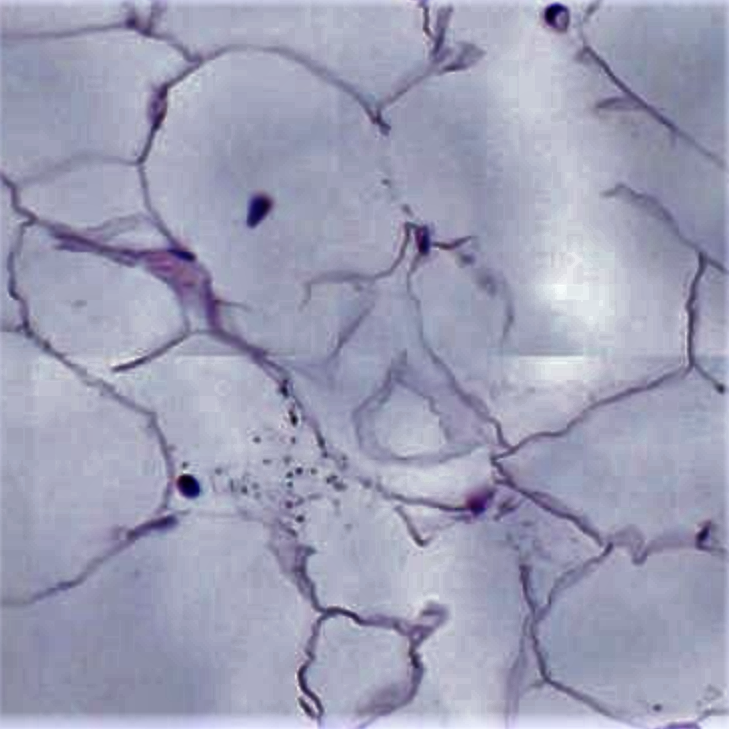
\includegraphics[width=0.98\textwidth]{backdp/artifact_scanner_stitching.png}
    \caption{}
    \label{fig:backdp:artifacts:scanning1}
  \end{subfigure}%
  \begin{subfigure}[t]{0.32\textwidth}
    \centering
    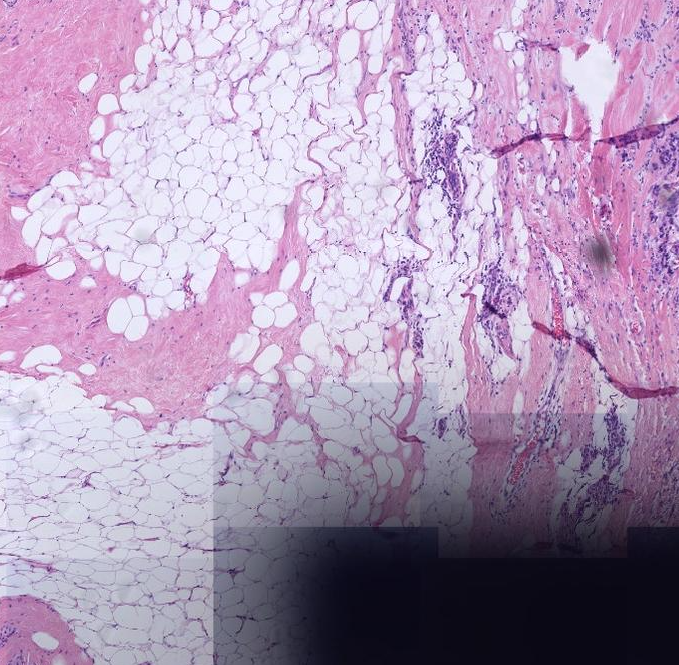
\includegraphics[width=0.98\textwidth]{backdp/scanning_artifact.png}
    \caption{}
    \label{fig:backdp:artifacts:scanning2}
  \end{subfigure}%

  \caption{\textit{Autolysis artifacts}: \ref{fig:backdp:artifacts:autolysis1} (poor cellular differentiation), \ref{fig:backdp:artifacts:autolysis2} (tissue separation). \textit{Microtomy artifacts}: \ref{fig:backdp:artifacts:microtomy1} (nick or blemish in the blade), \ref{fig:backdp:artifacts:microtomy2} (calcification pushed through the tissue by the blade). \textit{Folding artifact}: \ref{fig:backdp:artifacts:folding}. \textit{Staining artifact}: \ref{fig:backdp:artifacts:staining}. \textit{Scanning artifacts}: \ref{fig:backdp:artifacts:scanning1} (stiching issue), \ref{fig:backdp:artifacts:scanning2} (scanner failed to capture part of the tissue) \\ (sources: \ref{fig:backdp:artifacts:autolysis1}, \ref{fig:backdp:artifacts:autolysis2} \parencite{taqi2018review}; others from Cytomine).}
  \label{fig:backdp:artifacts:all}
\end{figure}

\begin{figure}
  \centering
  \begin{subfigure}[t]{0.48\textwidth}
    \centering
    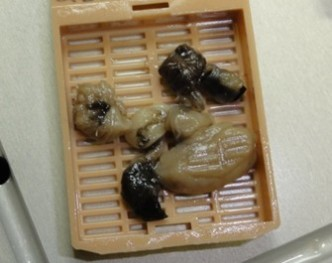
\includegraphics[height=150pt]{backdp/cassette.jpg}
    \caption{Cassette with fixated samples (source: \parencite{stidworthy2011getting})}
    \label{fig:backdp:cassette}
  \end{subfigure}\quad
  \begin{subfigure}[t]{0.48\textwidth}
    \centering
    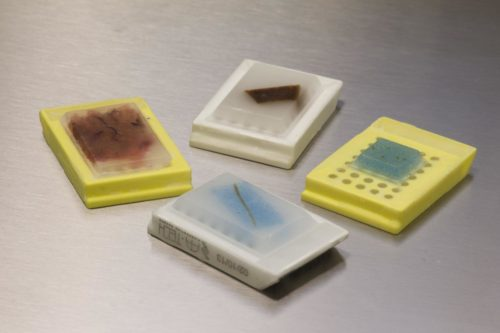
\includegraphics[height=150pt]{backdp/cassette-parrafin.jpg}
    \caption{Cassette with paraffin-embedded samples (source: \parencite{img:cassetteparrafin})}
    \label{fig:backdp:cassette-paraffin}
  \end{subfigure}
  \caption{Tissue cassettes.}
\end{figure}

\subsection{Embedding, microtomy and glass-slide application}
\label{ssec:backdp:embedding}

At this point, the sample in the cassette has been infiltrated with paraffin. The next step consists in embedding the infiltrated sample in a block of paraffin to allow easier cutting. The sample is placed in a small container which will serve as a mold for casting the block of paraffin. The cassette is then directly placed on top of the container so that, when the block solidifies, it is attached to the back of the cassette (see Figure \ref{fig:backdp:cassette-paraffin}). When it has indeed solidified, the sample can now be cut into thin slices to be applied on the glass slides. Cutting is performed with a dedicated tool called a \textit{microtome} (see Figure \ref{fig:backdp:microtome}). Operated by a technician, the microtome allows slices to be cut to an extremely small and precise thickness of around 3 or 4 $\mu m$. The slices are then floated onto a water bath which helps mouting them on glass slides. 

There exist automated embedding machines, but microtomy remains mostly manual. Although modern microtomes are equipped with automation features making them more ergonomic and convenient to use, they are still operated by technicians. There exist commercial systems that automatically process paraffin-embedded samples to produce unstained slides without human intervention but, to the best of our knowledge, these systems are not widespread and this step is still mostly performed by technicians. 

\begin{figure}
  \centering
  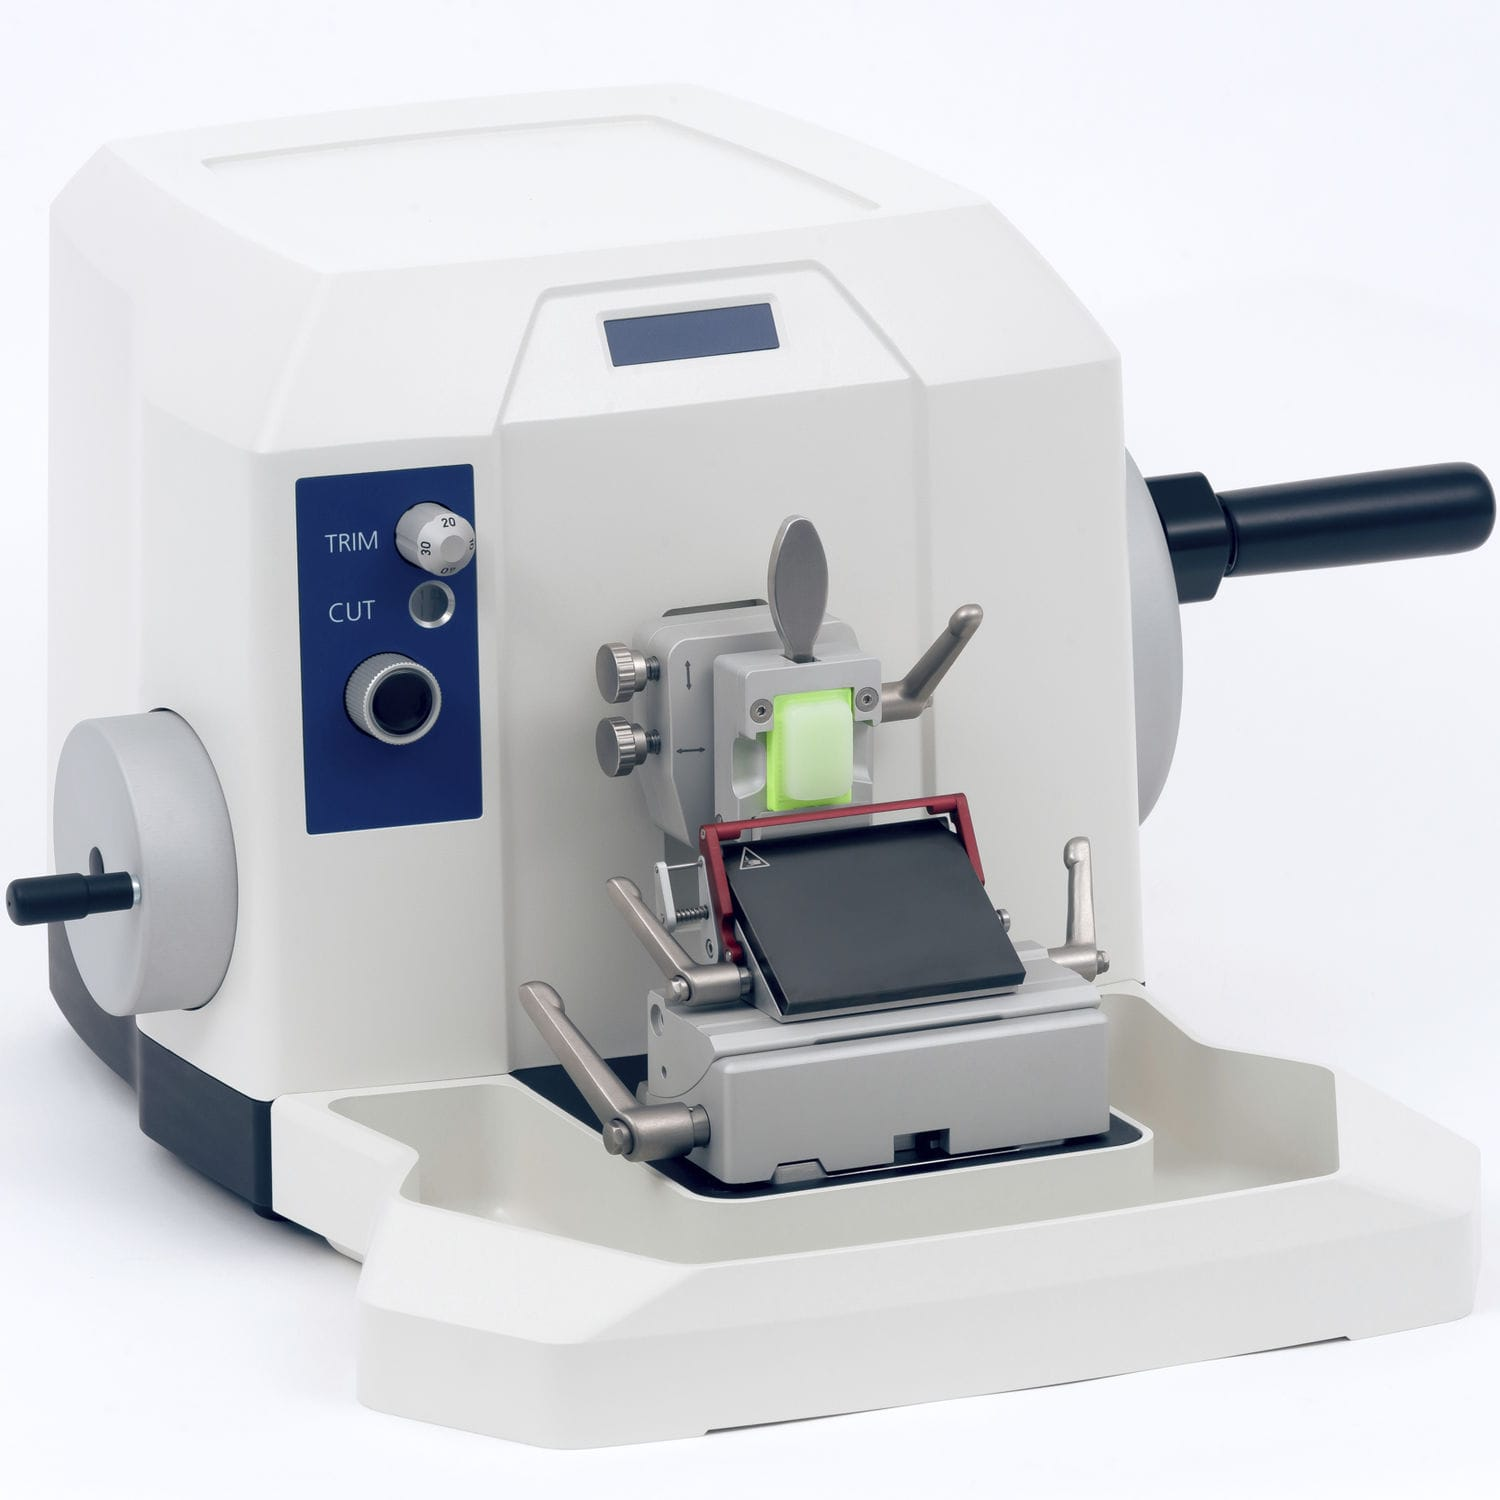
\includegraphics[width=0.5\textwidth]{backdp/microtome.jpg}
  \caption{A microtome}
  \label{fig:backdp:microtome}
\end{figure}

These steps should be performed carefully not to introduce artifacts. For instance, a warm and soft paraffin block, a dull microtome blade or a calcification in the tissue can cause compression artifacts (\ie tissue displacement causing material accumulation). A calcificaiton is solid calcium deposit present in the tissue that the blade cannot cut through. This deposit is therefore pushed through the tissue, compressing underlying tissues. Another possible source of artifact is contamination of the water bath with previous samples, hair or dust which can in turn contaminate the floating slices.   

\subsection{Staining}
\label{ssec:backdp:staining}
Mounted tissue slices are almost completely transparent which would prevent any meaningful analysis. They must therefore be stained to highlight structures of interest (see Figure \ref{fig:backdp:stainedvsnonstained}). Similarly as for dehydratation, this process consists in immersing the slide into a succession of stainning solutions. The nature of these solutions will depend on the content that should be highlighted for the future analysis. The most common and standard staining in histology is called \acrfirstit{heeo}. Hematoxylin stains nucleic acids in a deep blue-purple color (typically cell nuclei) and eosin nonspecifically stains proteins in a pink color (typically extracellular matrix and cytoplasm). The \acrshort{heeo} stain, although most common, is not the only available. There exist many other staining techniques such as \acrfirstit{ihc} which exploits the binding nature of some antibodies with specific proteins. Markers can then be used to highlight the antibodies, hence the proteins of interest they have bound with. Because the \acrshort{ihc} staining can be very selective, a counterstain (\eg hematoxylin) is often applied to highlight   the rest of the tissue. Counterstain is particularily important when different slices of a tissue stained with different techniques must be compared together because it helps matching the slices spatially. An example of a tissue stained with \acrshort{heeo} and \acrshort{ihc} is given in Figure \ref{fig:backdp:heeo-ihc}. When the sample has been stained and cleaned from remaining excess of staining solutions, one must apply a cover slip on the sample in order to ensure that sample lies in one single plane as the focal plane of microscopes and scanners is usually quite narrow. The cover slip also protects the sample from external contamination and degradation. 

\begin{figure}
  \centering
  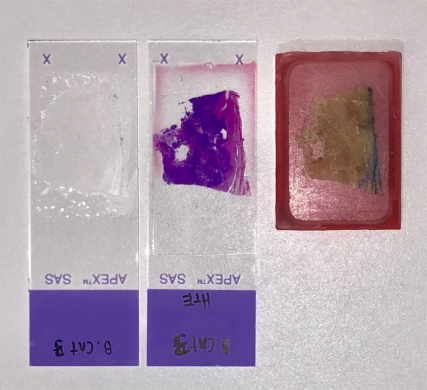
\includegraphics[width=0.6\textwidth]{backdp/staindvsnonstained.png}
  \caption{\textit{Left:} an unstained tissue section mounted on a glass slide. \textit{Middle:} \acrshort{heeo}-stained section coming from the same tissue. \textit{Right:} the source tissue embedded in a paraffin block \\ (source: \parencite{abbasi2019all})}
  \label{fig:backdp:stainedvsnonstained}
\end{figure}

The choice of a staining and its clean application are crucial for an efficient analysis. The staining baths can become contaminated with samples, by-products resulting from chemical reactions (\eg precipitation or crystallization of chemical components resulting in the presence of pigments in the sample) or external objects (\eg hair, dust). The baths tend to degrade over time as moving slides from one bath to another transfer some staining solutions as well. The degradation of the staining solutions can cause variation in staining intensities between earlier and later samples. The bath duration is important for proper staining and bathing samples for less or more time than recommanded can respectively cause under- or over-staining. Moreover, insufficient cleaning after staining can leave spots of stain on the slide. Improper application of the cover slip can for instance cause the presence of air bubbles. Nowadays, the staining process can be automated with automated slide stainers. These systems move the slide automatically from a bath to the next ensuring stable dipping durations for each stain.

\begin{figure}
  \centering
  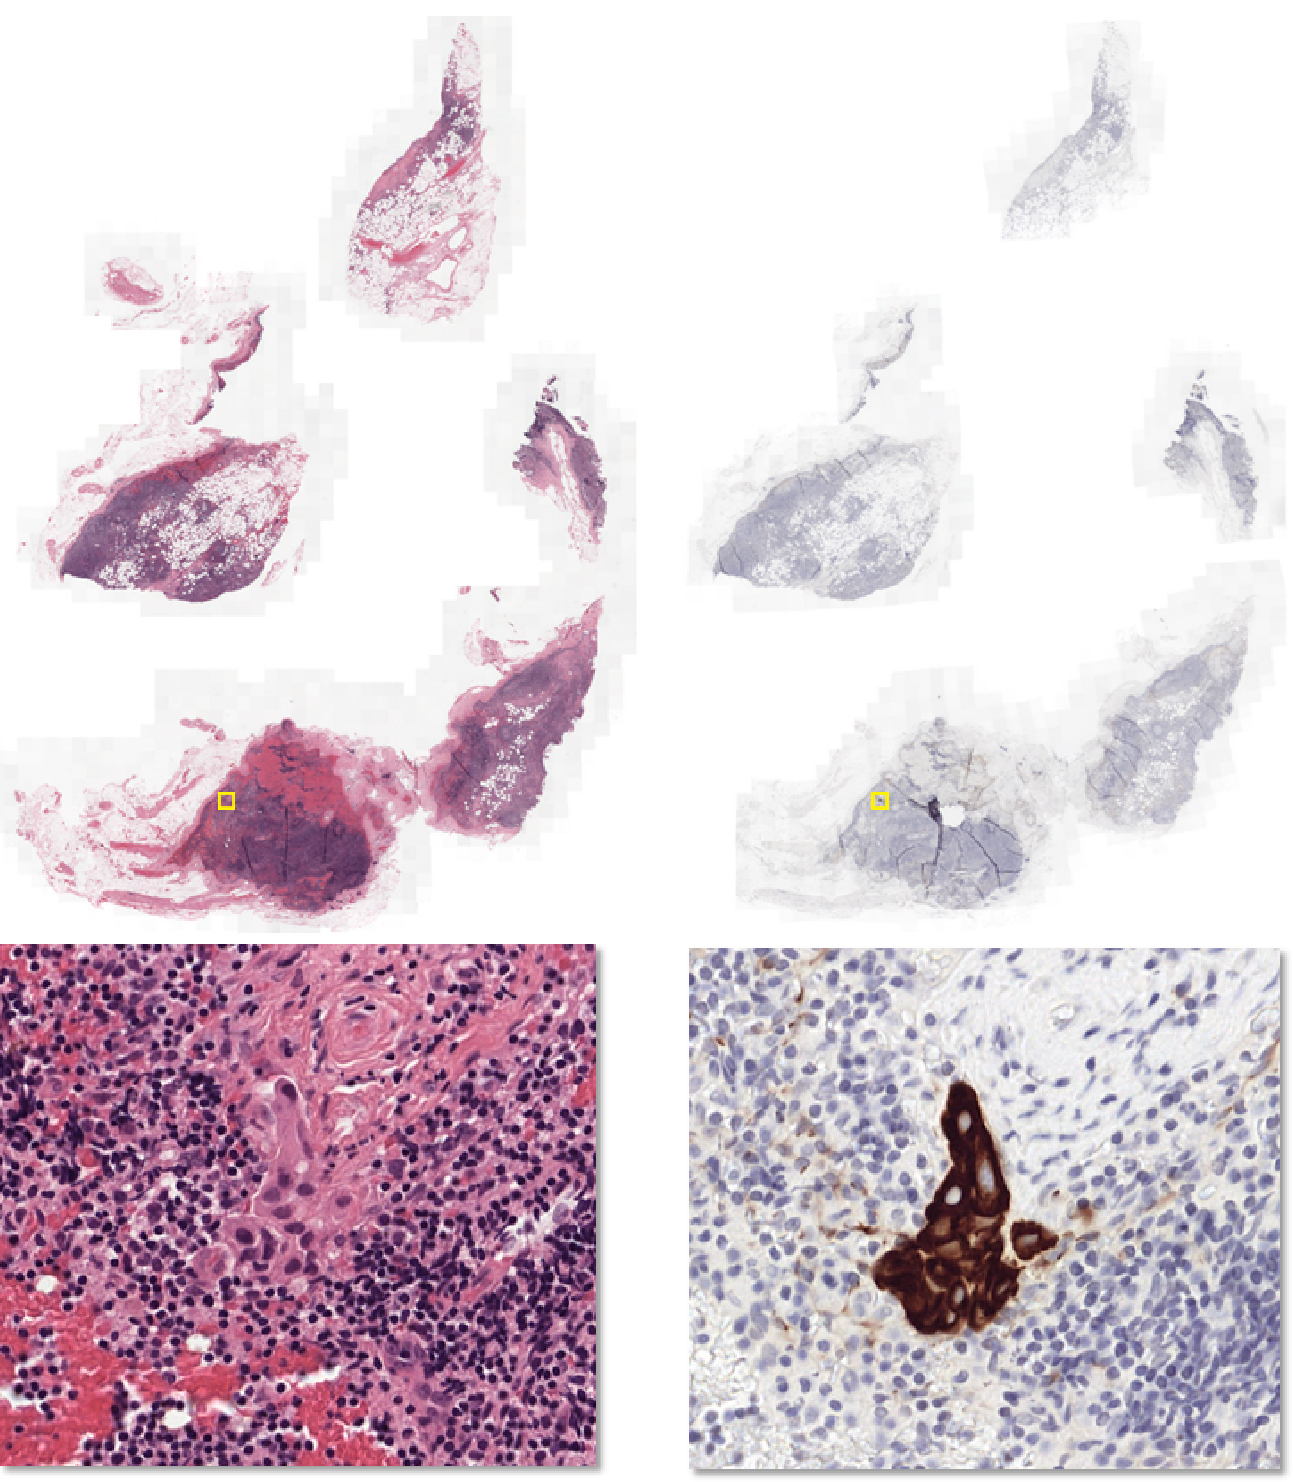
\includegraphics[width=0.5\textwidth]{backdp/heeo-ihc.jpg}
  \caption{Two slices of the same tissue stained with \acrshort{heeo} (left) and \acrshort{ihc} (right). \\(source: \parencite{litjens2018camelyon})}
  \label{fig:backdp:heeo-ihc}
\end{figure}

\subsection{Scanning}
\label{ssec:backdp:scanning}

A glass slide coming out of the staining process described in Section \ref{ssec:backdp:staining} is ready to be analyzed with an optical microscope but can also be digitized by a slide scanner into a \acrshort{wsi}. In this section, we will briefly describe few key elements related to slide scanning. A more thorough technical presentation and discussion of scanning technologies can be found in \parencite{patel2021contemporary}. 

Scanners are equipped with high-precision lenses and sensors allowing them to generate very high-resolution images required for a proper analysis. Magnification and resolution are two popular metrics used to describe the visual quality of the resulting image. Magnification advertised by scanner vendors refers to the maximum size of the objects in the scanned image with typical values being $\times$20 or $\times$40 (\ie objects appear 20 or 40 times larger than they actually are). Resolution determines the extent to which smaller objects can be resolved. Resolution is reported for a given magnification level and often lies around 0.25 $\mu$m/pixel at $\times$40 for modern scanners but higher magnification and resolution are possible. These magnifications are standard and, coupled with an adequate resolution, are usually sufficient for routine analysis of \acrshort{heeo} or \acrshort{ihc} slides \parencite{zarella2019practical}.

\begin{figure}
  \centering
  \begin{subfigure}[t]{0.48\textwidth}
    \centering
    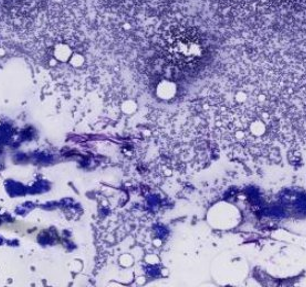
\includegraphics[height=190pt]{backdp/magres_x1.25_cell.png}
    \caption{$\times$1.25, 7.24 $\mu$m/pixel}
  \end{subfigure}
  \begin{subfigure}[t]{0.47\textwidth}
    \centering
    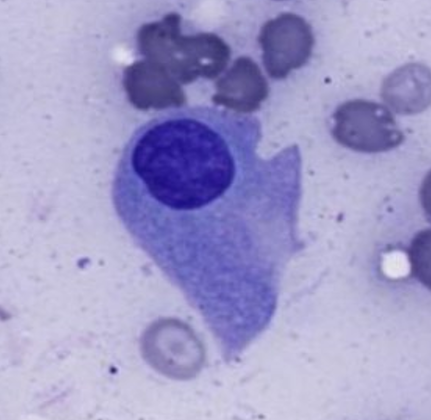
\includegraphics[height=190pt]{backdp/magres_x40_cell.png}
    \caption{$\times$40, 0.226 $\mu$m/pixel}
  \end{subfigure}
  \caption{Two images (approximately 200 $\times$ 200) extracted from the same WSI at different magnification and resolution (reported in subcaptions). They are both centered on the same cell.}
\end{figure}

Given the need for high magnification and resolution, it is not possible to capture the whole slide in a single shot with currently available sensors. Therefore, scanners typically capture a sample step by step either tile by tile or in a in-line fashion and then assemble together the different parts using a stitching algorithm. Obviously, as a slide is scanned in several shots, the scanner must ensure that focus is correct for all the shots in order to avoid blur. Common focus strategies are for instance re-focusing every tile, or every $n^{\text{th}}$ tile. When it comes to the focus strategy, there is usually a trade-off between scanning time and focus precision: focusing every tile allows for ideal focus but takes time, whereas focusing every $n^{\text{th}}$ is faster but incurs a risk of incorrect focus and blur between the re-focusing steps. Modern scanners implement efficient strategies to reduce the scanning time per slide which nowadays ranges from 30 seconds to several minutes (at $\times$20 or $\times$40 magnification). These strategies include improved focus strategies and automatic tissue detection allowing to skip the empty parts of the slide during scanning. Most scanners also allow to load batches of few hundreds of slide at once therefore reducing the time spent by the operator interacting with the machine.

For histology, it is usually sufficient for scanners to scan one focal plane of the slide (\ie that of the tissue slice). For cytology, however, it is not always enough. Indeed, the slide preparation process for a cytology sample differs and the material are not always aligned within a single focal plane. With an optical microscope, it is possible to navigate continuously over the focal planes by adjusting the lenses positions. When it comes to scanning such samples, one has to resort to a technique called "\textit{z-stacking}". It consists in capturing the material at different depths along the $z$-axis. This process can be significantly longer than single focal plane scanning, as it multiplies this time by the number of slices of the stack. The result is a finite number of images which can be viewed in different ways (\eg one by one, grid view, as a video sequence, \etc.) but do not offer the simplicity or continuous exploration provided by optical microscope for this task. 

Scanning can also introduce artifacts including stiching problems (\ie misalignment between scanned tiles or lines), blur due to incorrect focus, tissue detection failure causing parts of the slide to be missing from the \acrshort{wsi}. The scanner should obviously remain as clean as possible to avoid external components to pollute the image (\eg dust, glass shards, hair, \etc.). 

\subsection{File formats and compression}
\label{ssec:backdp:storingviewing}

For each glass slide, a scanner generates one or more files to store the image data but also any metadata related to the case (information or identifiers of laboratory, patient, specimen, staining, \etc.). How the data is organized in such a file is specified by a \textit{file format} of which there exist many. Some file formats are closed and proprietary (\eg scanner- or vendor-specific file formats) but others have open specifications (\eg DICOM, OME-TIFF). The most involved formats usually combine a descriptive part to store case-related metadata using, for instance, the XML language (\eg in OME-TIFF) and a subfile format for the image itself (\eg TIFF). 

Regarding the internal structure of the latter, the image is usually splitted into a set of tiles (\eg 1024 $\times$ 1024) rather than being stored as a single image array. The file contains metadata to provide efficient access to these tiles. This organization makes sense because, in practice, one rarely has to load the whole image in memory at full resolution at once which, given the size of a raw image (\eg Figure \ref{fig:backdp:pyramidalimage}), would be impossible on most computers anyway. It is however a common use case for a practitioner to look at an entire slide (or a large region of interest) at a lower magnification and resolution. Downsizing, downsampling and aggregating tiles to obtain a low resolution view of a slide (or a region of interest) is an expensive operation and cannot realistically be performed on-the-fly without significantly increasing loading times. Therefore, a typical image files also stores versions of the image at different zoom levels. The $i^{\text{th}}$ zoom level ($i \in \mathbb{N}_0$) is a version of the image which has been downsized by a factor $2^i$ (or $3^i$, $4^i$ depending on the image format). The number of zoom levels varies depending on the size of the image at full resolution and is such that the image at the lowest zoom level (\ie largest $i$) has a reasonably low size (\eg when it fits in a single tile). Similarly as for zoom level 0, other zoom levels are stored as set of tiles. Such a file is called \textit{pyramidal} because of this structure (see Figure \ref{fig:backdp:pyramidalimage}).

\begin{figure}
  \centering
  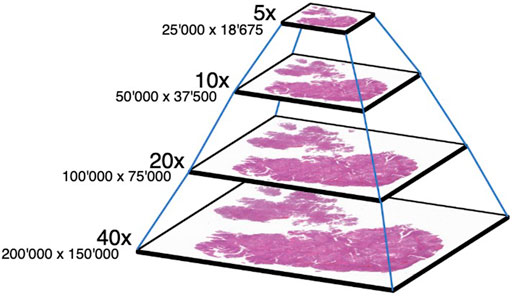
\includegraphics[width=0.75\textwidth]{backdp/pyramidalimage.jpg}
  \caption{Pyramidal view of a whole-slide image (source: \parencite{marini2022multi_scale_tools})}
  \label{fig:backdp:pyramidalimage}
\end{figure}

A whole-slide image file is not a lightweight one. For example, a raw $10^5 \times 10^5$ RGB image (3 bytes per pixels) contains 30 gigabytes of information. This is massive and not scalable if one has to consider the multitude of slides to be scanned and stored by an hospital for instance. Therefore, compression algorithms are very frequently used to reduce the size of image files. Popular choices are JPEG (lossy compression) and JPEG2000 (lossless compression). Compared to its lossless counterpart, lossy compression allows for better compression rate and disk usage reduction. However, the loss of information results in visual alteration that become more and more severe as the compression rate increases. Therefore, lossy compression should be used carefully to avoid destroying image features relevant to the analysis. 

\subsection{Visualization and hardware considerations}
\label{ssec:backdp:visualization}

An image file is not worth much if it cannot be viewed. Nowadays, there exist many open or proprietary software and tools for visualizing \acrshort{wsi}. Some are desktop applications designed to run on personal computer and workstations (\eg QuPath \parencite{bankhead2017qupath}, ASAP \parencite{cpg2022asap}) or directly provided by scanner vendors to run on dedicated hardware alongside the scanner. Some others are web-based (\eg Cytomine \parencite{maree2016collaborative}, OMERO \parencite{allan2012omero}) for which the viewer can be accessed through a web browser and content is served over the HTTP protocol. The most popular tools are not limited to a viewer but usually include many more features. For instance, Cytomine includes image annotation tools, integration of computer vision and \acrlong{ml} algorithms, authentication, project-based content organization, an \acrshort{api} to interact with data programmatically,...

Whereas it is included by-design in web-based tools, remote slide viewing is also possible with some desktop applications. This feature is particulary important in a laboratory environment. Without it, the system would need to download an entire \acrshort{wsi} file before being able to display. This would add a significant latency in the slide reviewing process. Remote slide viewing allows for a seamless and more efficient interaction between the practitioner and the viewing system.

Beyond software, hardware considerations are important for efficient viewing, especially when implemented at the scale of a laboratory or pathology service \parencite{temprana2022digipatics}. Personnal workstations should be equipped with a quality screen able to render image without loss of quality (color and resolution). They also must be equipped with adequate computing resources (memory and \acrshort{cpu}/\acrshort{gpu}) in particular if analysis algorithms are supposed to be executed on them. The network should be robust enough to support the exchange of information (\ie download and upload of large files and data). Servers should have enough disk space to store the digitized slides and data and implement mechanisms in order to minimize the risk of data corruption or loss. 

% \TODO{variations of appearance due to using a tool vs another \parencite{cheng2020evaluating} ??}

\subsection{Discussion}

As presented in the previous sections, the preparation process has a significant impact on the final quality of a slide. Every step in the process introduces variability and has a chance of creating artifacts that can be both harmful to the analysis. Fortunately, automation reduces significantly the variability and makes the risk of artifacts acceptably low, although not absent. The dehydration, paraffin embedding and staining steps can all be automated with dedicated machines nowadays but microtomy remains mostly manual due to the high-precision requirements of the process. For scanned slide, there exist automated quality control tools such as HistoQC \parencite{janowczyk2019histoqc} or PathProfiler \parencite{haghighat2021pathprofiler} to verify that a \acrshort{wsi} has a sufficient quality to be considered for analysis. 

The preparation process also impacts significantly the diagnosis time as overall, from fixation to scanning, it can take from 12 to 24 hours (sometimes more) to obtain a slide depending on the nature and state of the original specimen. There exist faster processes such as cryosectioning (\ie the sample is frozen then sectioned) for intraoperative consultation during which a surgeon requests an analysis to decide how to proceed with a surgical operation. Such process can provide an answer within the hour but the resulting slides are usually of lesser quality than traditionally prepared histological slides.

\section{Whole-slide analysis}
\label{sec:backdp:typicalanalysistasks}

When a slide has finally been prepared, a pathologist, a biologist or a technician can take over and start the analysis, whether on a computer screen or through the lenses of an optical microscope. There exist many active research domains which rely on slide analysis. Similarly, there exist many pathologies that can be discovered from the same source. For the sake of simplicity, the remainder of the section will focus on oncology and cancer diagnosis. In this field, one of the most frequent condition that has to be evaluated is malignancy of tumors. The indicators of malignancy can vary greatly from a disease to another and even from one type of cancer to another. The approach of the slide by the pathologist and the analysis can therefore vary accordingly.

Two important tools for diagnosis and prognosis of cancer are grading and staging systems. A grading system is a set of mostly objective criteria for evaluating how abnormal cancer cells and tissues are compared to their healthy counterparts. Similarly, a staging system defines a set of criteria for quantifying the dimensions of the primary tumor and determining how far the cancer has spread in the patient's body. These criteria can be quantitative (\eg cell counts, tumor area dimensions) or qualitative (\eg cell or tissue morphology, presence of metastases) and consider macroscopic or microscopic elements. Beyond grading and staging, slide analysis can also provide direct information for establishing a proper treatment. For instance, localizing a malignant tumor in its support tissue can be important for guiding a future surgical operation. 

All the types of tasks involved in slide analysis are not equal. They have varying degrees of complexity and tediousness. Some tasks are rather simple but take a significant amount of time (\eg counting mitosis, see Section \ref{ssec:backdp:analysis_mitotic_count}), others require strong focus for an extended period of time which increases the risk of error (\eg thyroid nodule malignancy, see Section \ref{ssec:backdp:analysis_thyroid}). Moreover, some diagnoses require to screen more than just one slide, in which case the volume of information to review can be significant. 

When a task has to be performed frequently and is tedious, error-prone or involves reviewing a large amount of data, there is a great potential for \acrlong{cpath} methods to improve analysis quality and speed. These methods can either provide quantitative or qualitative information that directly contributes to the diagnosis or simply assists the practitioner during the reviewing process. % (\eg image registration, see Section \ref{ssec:backdp:analysis_registration}). 

Beyond automating existing tasks, \acrlong{cpath} could also give rise to new approaches and standards for diagnosis. For instance, computational methods could be used to extract new descriptive features such as exhaustive statistics about cell types and structure in a sample or new cell morphology descriptors. This information could be used alongside non-imaging data and correlated to patient outcome \parencite{abels2019computational}. 

In the longer term, new computational methods coupled with new imaging techniques could make obsolete the slide preparation process as it is performed now as well as the current diagnosis systems based on histology and cytology. Indeed, in the future, entire specimen could be scanned directly to produce 3D volumes with slide-free microscopy techniques \parencite{np2017histopathology, liu2021slide}. These image volumes could be analyzed directly by computational methods to provide fast and hopefully reliable indicators for pathologists to diagnose cases in a shorter time frame than ever before. However, it will take a significant amount of time before such technology is sufficiently developed, validated and becomes reliable enough to be used in clinical practice on a daily basis. 

In the following sections, we provide some examples on diagnosis tasks that would greatly benefit from automation with computational methods. For each of them, we also provide examples of contributions of the \acrlong{cpath} community to the automation of these tasks. The datasets presented in these sections were used in the contributions of the thesis. 

\subsection{Mitotic count}
\label{ssec:backdp:analysis_mitotic_count}

Mitosis is one of the phases of the cell cycle during which the chromosomes (replicated in a previous phase) are separated into two new nuclei. Tumor often exhibits a larger mitosis rate compared to healthy tissues. Many grading systems therefore use a measure of the mitosis rate as an indicator of cancer severity. For instance, the Bloom-Richardson system \parencite{roychowdhury2022bloomrichardson} for histologic grading of breast cancer includes mitotic count as one of its three indicators. In particular, mitosis must be counted in 10 fields of view. The final grade is determined based on a point system. Each indicator provides 1 (least severe) to 3 (most severe) point(s) which are added together (3-5 pts = grade I, 6-7 pts = grade II and 8-9 pts = grade III). For the mitosis indicator, 1 point is given if the mitotic count is 5 or less, 2 points if it is between 6 and 10 and 3 points if it is 11 or more\footnote{The recommanded numbers might change based on the microscope used for the analysis.}. 

Counting mitosis is not necessarily complicated but it is cumbersome. It is no surprise that \acrlong{cpath} methods have been investigated to automate the task. For example, in 2014 was organized the MITOS-ATYPIA-14 challenge \parencite{roux2014mitos} where participants had to come up with the best \acrlong{ml} model to count the number of mitosis in different field of views (see Figure \ref{fig:backdp:mitos_atypia}). In addition to the mitotic count, they had to predict a global nuclear atypia score for each field of view, nuclear atypia being another indicator of the Bloom-Richardson system. 

\begin{figure}
  \centering
  \begin{subfigure}[t]{0.48\textwidth}
    \centering
    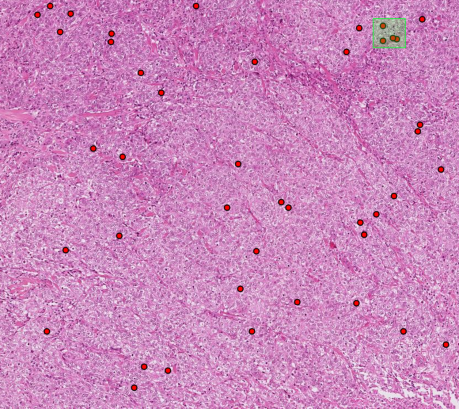
\includegraphics[height=190pt]{backdp/mitosis_zoomout.png}
  \end{subfigure}
  \begin{subfigure}[t]{0.48\textwidth}
    \centering
    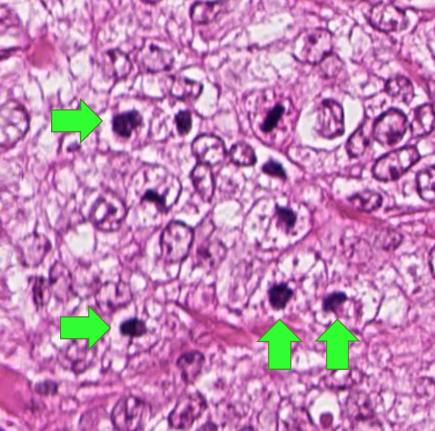
\includegraphics[height=190pt]{backdp/mitosis_zoomin.png}
  \end{subfigure}
  \caption{\textit{Left:} a training image provided for the MITOS-ATYPIA-14 challenge viewed from the Cytomine viewer. Red dots are mitosis present in this image. \textit{Right:} A close up view of four mitosis (in the green square from the left image).}
  \label{fig:backdp:mitos_atypia}
\end{figure}

\subsection{Breast cancer staging and sentinel lymph nodes}
\label{ssec:backdp:analysis_camelyon}

Axillary lymph nodes are structures of the immune system located near the armpit. They drain a large proportion of the lymph coming out of the breast. They contain lymphocytes and constitute a barrier that eliminates bacteries, viruses and other foreign particules (including metastases) from the lymph. Because they are the first recipient of metastases originating from breast tumors, these lymph nodes are an important element to consider when staging breast cancer. In particular, in the context of $TNM$, a standard internationally accepted cancer staging system, the $pN$-stage \parencite{reisenbichler2022tmnstagingbreast} quantifies cancer spread through the presence of metastases in regional lymph nodes. Its histological evaluation requires to screen one section of up to 10 axillary lymph nodes and several sections of the ``sentinel'' lymph node which is the most likely to contain metastases \parencite{weaver2010pathology}. Sometimes, additional slides counter-stained with \acrshort{ihc} must be analyzed to confirm the diagnosis. The staging system requires to evaluate the number of nodes contaminated with metastases and the dimensions of these metastases (\ie their size and the number of cells they contain).

Evaluation of the $pN$-stage has many characteristics that qualifies it to be a good candidate for automation: it is time-consuming, tedious and error-prone. The computational pathology community has therefore considered this problem notably through the Camelyon16 and Camelyon17 challenges \parencite{litjens2018camelyon}. For the first iteration of the challenge, the participants had to predict a slide-level $pN$-stage. For the second iteration, the organizers moved to a patient-level prediction. The participants were provided with 899 training and 500 testing \acrshort{wsi}s which were collected in 5 differents hospitals and medical centers from the Netherlands. All training slides were also coming with a slide level $pN$-stage label. Moreover, 209 of those \acrshort{wsi}s contained detailed hand-drawn contours for all metastases (see Figure \ref{fig:backdp:camelyon_sample}). The top-performing solutions typically used a combination of techniques and algorithms including traditional computer vision pre- and post-processing methods, \acrlong{dl} to segment the metastases and rule-based or random forests methods to predict the final stage. 

This challenge was a success as many teams participated despite the complexity of handling such a massive dataset (3 terabytes of slide data). The top-performing algorithms were quite successful at predicting the $pN$-stage. However, as stated by the organizers, the task was not adequatly solved and there was room for improvement \parencite{bandi2018detection} as a combination of the best algorithms still misclassified the $pN$-stage for 23 patients out of 100. 

\begin{figure}
  \centering
  \begin{subfigure}[t]{\textwidth}
    \centering
    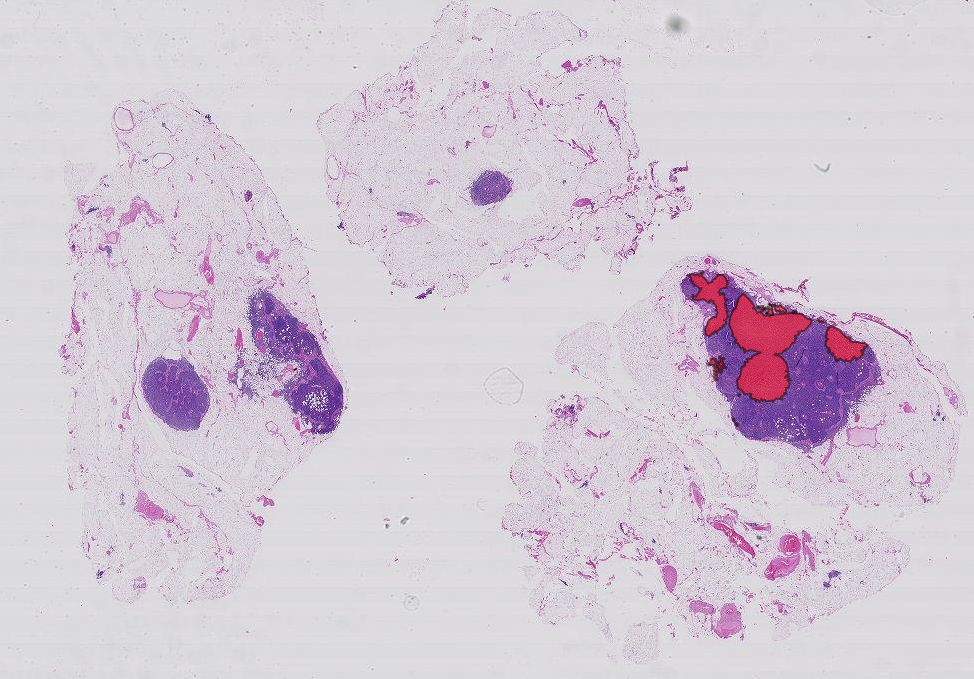
\includegraphics[width=\textwidth]{backdp/camelyon_lymphnode.png} 
  \end{subfigure}\\
  \vspace{1cm}
  \begin{subfigure}[t]{0.48\textwidth}
    \centering
    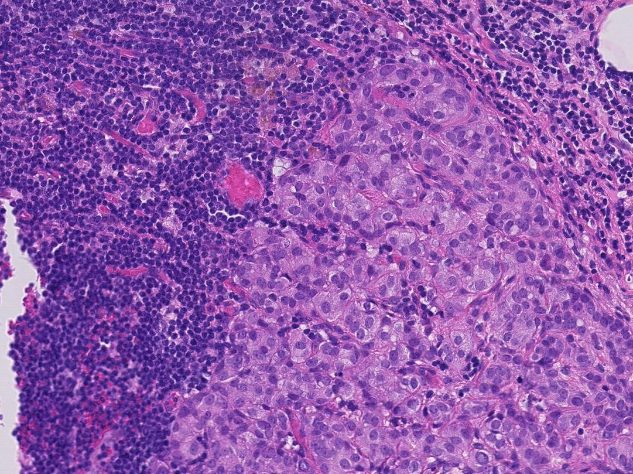
\includegraphics[height=150pt]{backdp/camelyon_metastase_noannot.png}
  \end{subfigure}
  \begin{subfigure}[t]{0.48\textwidth}
    \centering
    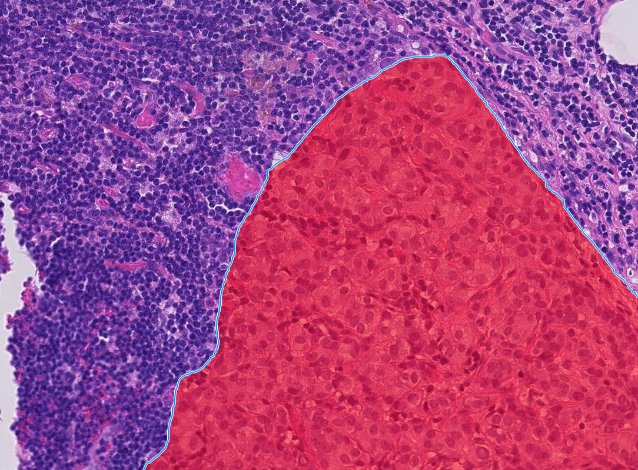
\includegraphics[height=150pt]{backdp/camelyon_metastase_withannot.png}
  \end{subfigure}
  \caption{A \acrshort{wsi} from the Camelyon16 challenge training set viewed from the Cytomine viewer. \textit{Top:} the whole-slide image with metastases highlighted in red. \textit{Bottom:} A close-up view of a metastase with (\textit{right}) and without (\textit{left}) annotation mask.}
  \label{fig:backdp:camelyon_sample}
\end{figure}

\subsection{Thyroid nodule malignancy}
\label{ssec:backdp:analysis_thyroid}

A thyroid nodule is a small lump that can form within the thyroid gland. Most nodules are benign but up to $5\%$ of them are malignant \parencite{yeung2008management}. Malignancy diagnosis is based on a wide variety of information including patient history (past exposure to radiation, family history of thyroid cancer, \etc.) and different technical examinations (\eg echography or radiography). A crucial step in the process is the \acrfirstit{fnab} during which cell material is extracted from the nodule. The resulting cytology sample is smeared on a glass slide (this slide preparation process is different from the one described in Section \ref{sec:backdp:wsi}), stained and examined under a microscope. Cytology analysis is an integrant part of the Bethesda diagnosis system \parencite{bychkov2022bethesda} which grades a nodule into six categories going from nondiagnostic (TBS I) and benign (TBS II) to malignant (TBS VI). One of the elements that define the TBS category is the presence of cells with intranuclear inclusions (see Figure \ref{fig:backdp:thyroid_inclusion}) which are highly suggestive of malignancy \parencite{arena2014intranuclear}. Relatively to the size of a slide, these cells are tiny and the problem of finding them comes down to searching a needle in a haystack (see Figure \ref{fig:backdp:thyroid_needle_haystack}). However, these cells are not the only indicators of thyroid cancer and considering this is only a part of what must be investigated in a thyroid nodule smear, it would greatly benefit from the use of computational methods. An algorithm could either directly help pathologists in finding the cells or provide a more comprehensive diagnosis system that would make the search of such cells irrelevant. 

Although the earliest application of \acrlong{ai} to nodule malignancy assessment dates back to the 1990s \parencite{karakitsos1999learning}, the topic is still quite overlooked and currently available algorithms are mostly benign \vs malignant classifiers \parencite{kezlarian2021artificial} which are too simplistic to be used in clinical settings. One recent contribution, however, considered the problem of predicting directly one of the categories of the Bethesda diagnosis system \parencite{elliott2020application}. This approach is more realistic and in-line with the pathologists' diagnosis process but still requires further examination to assess its wider applicability.

\begin{figure}
  \centering
  \begin{subfigure}[t]{0.225\textwidth}
    \centering
    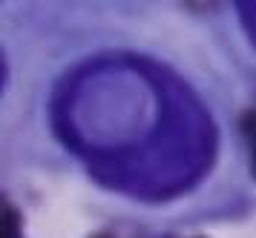
\includegraphics[height=80pt]{backdp/incl1.png}
  \end{subfigure}
  \hspace{0.1cm}
  \begin{subfigure}[t]{0.225\textwidth}
    \centering
    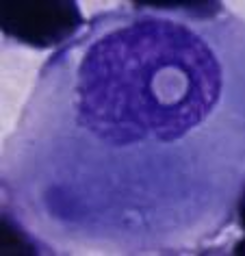
\includegraphics[height=80pt]{backdp/incl2.png}
  \end{subfigure}
  \hspace{0.1cm}
  \begin{subfigure}[t]{0.225\textwidth}
    \centering
    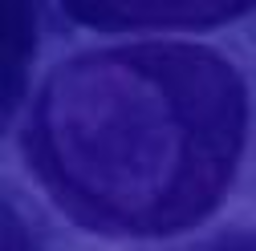
\includegraphics[height=80pt]{backdp/incl3.png}
  \end{subfigure}
  \hspace{0.1cm}
  \begin{subfigure}[t]{0.225\textwidth}
    \centering
    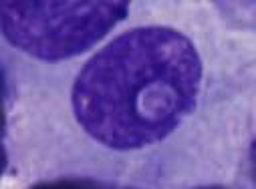
\includegraphics[height=80pt]{backdp/incl4.png}
  \end{subfigure}
  \caption{Example of cells with an intranuclear inclusion from thyroid nodule \acrshort{fnab} smears.}
  \label{fig:backdp:thyroid_inclusion}
\end{figure}

\begin{figure}
  \centering
  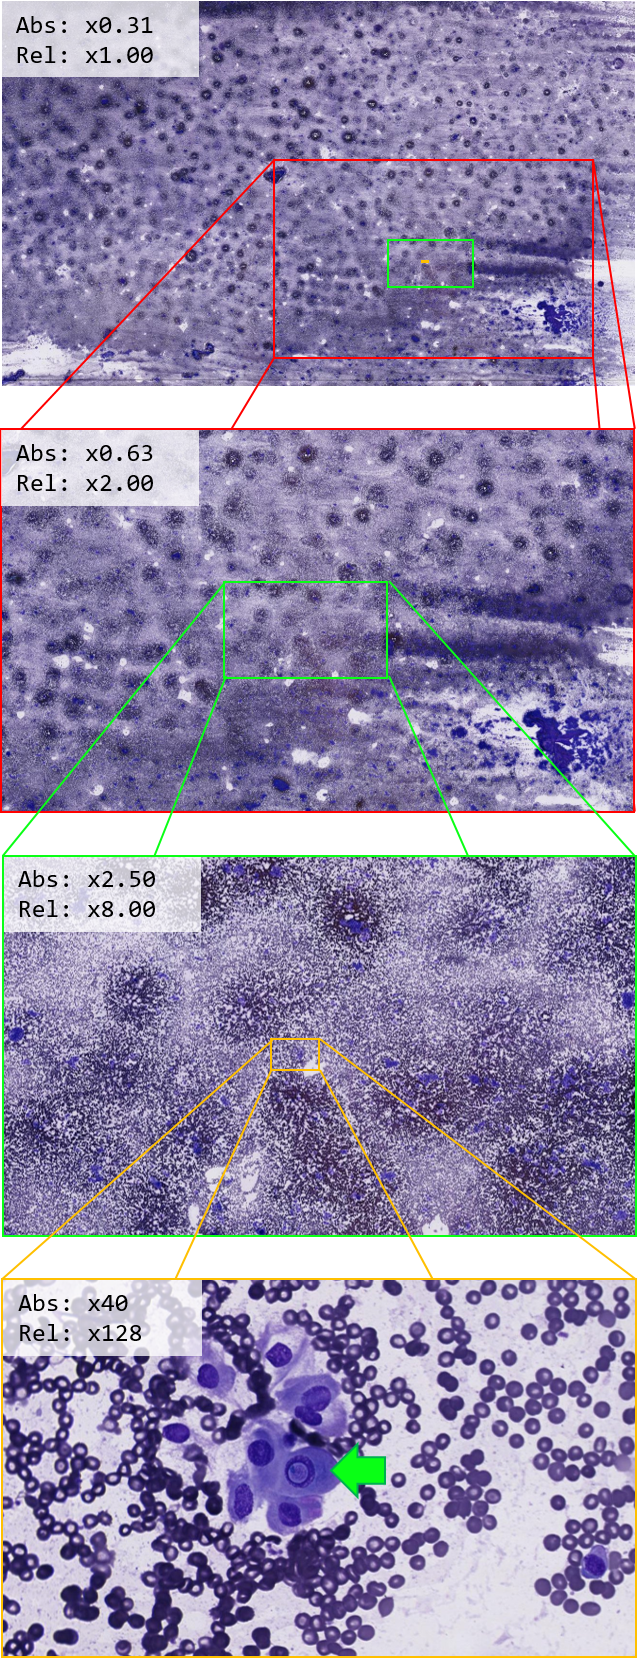
\includegraphics[height=21cm]{backdp/thyroid_needle_haystack.png}
  \caption{Views of a intracellular inclusion at different zoom levels. In the top left corners of each image are the absolute and relative magnification.}
  \label{fig:backdp:thyroid_needle_haystack}
\end{figure}



%\subsection{Registration}
%\label{ssec:backdp:analysis_registration}
%\TODO{illustrate with some of my datasets}


\section{Computational pathology and machine learning}
\label{sec:backdp:ml}

Digital pathology has opened the way for the application of \acrlong{ml} to automate analysis and diagnosis. Albeit promising, the application of \acrlong{ml} remains challenging for various reasons. In this section, we discuss some of these challenges then present some techniques that can be used, if not to overcome them, at least to alleviate them.

%  in Sections \ref{ssec:backdp:dataleakage} and \ref{ssec:backdp:datascarcity}

\subsection{Data leakage}
\label{ssec:backdp:dataleakage}

In Section \ref{ssec:backml:modelselinpractice}, we introduced the notion of data leakage that occurs when samples in different splits of a dataset are not independent from each other. Data leakage usually results in poor evaluation of the generalization performance, leading to a poor choice of hyperparameters. Obviously, this should be avoided at all cost especially when the prediction of this model impacts the patient diagnosis and treatment. It is worth noting that data leakage is considered an important obstacle for the application of \acrlong{ml} in biology and medicine in general, not only in \acrlong{dp} \parencite{ching2018opportunities}. 

In \acrlong{dp}, data leakage can occur in many, sometimes subtle, ways. Therefore, learning pipelines should be built carefully. One important potential source of data leakage is due to the fact that a whole-slide image does not only convey information about the tissue it contains but also about the slide preparation process (see Section \ref{sec:backdp:wsi}). For instance, staining solutions decay over time. Therefore, the staining intensity can reflect whether the sample has been dipped in a recently-changed or an heavily-used staining bath. When staining is performed manually, the intensity might also reflect the identity of the technician who performed the staining operation. Indeed, some technicians might dip slides for a little longer than others resulting in a stronger intensity. When a dataset is built by different laboratories, the origin of a slide is traceable due to differences in the slide preparation processes between the sites. 

These slide idiosyncracies are harmless as long as they are not correlated with the learning problem target. Whereas it might seem unlikely to happen, some simple though unfortunate choices can lead to correlation. For instance, supposing a problem of malignancy assessment, if one laboratory provides all the healthy samples and another all the malignant samples, there is significant risk that the learning algorithm would exploit the differences resulting from the preparation processes. This would obviously lead to poor generalization when the model will be applied to slide coming from another laboratory for instance. 
%This could occur similarly if malignant and healthy slides are provided by the same laboratory but the former are prepared in the morning and the latter in the afternoon.

The slide preparation process is not the only culprit for data leakage. Another possible source occurs at the patient level. \citeauthor{bussola2021ai} \cite{bussola2021ai} have empirically studied patient-wise and random dataset splitting strategies. They have shown that overfitting and data leakage indeed occur when splitting samples randomly.

% {test score worse for patient wise splitting than for tile wise splitting in the article. That's unexpected.}

In general, it is difficult to completely prevent data leakage as one does not always have control over the whole \acrshort{wsi} generation process. However, good practices surely help reducing the problem to an acceptable minimum. A detailed list of guidelines and good practices to reduce the risk of data leakage can be found in \parencite{maree2017need}. This includes collecting data as representative as possible of the different variations that could naturally occur during the generation process. For model evaluation and selection, splitting the dataset into subsets should be performed considering the characteristics of the samples that could correlate with the target (\ie patient, laboratory, technician, staining, equipement, time of the day/week, \etc.).

\subsection{About annotations}
\label{ssec:backdp:conceptannotation}

Annotations are important to train \acrlong{ml} models in a supervised manner. They provide information to the algorithm that can adapt the model to fit more accurately the target data. An annotation typically links two elements: an annotation construct and a semantic information. 

An annotation construct concerns the format of the annotation. For instance, in classification, the annotation is a label usually encoded as an integer. For object detection, a common construct is the bounding box framing an object of interest. In image segmentation, the construct is often a hand-drawn polygon covering all pixels belonging to a structure of interest. The semantic information links an annotation to the semantic of the tackled problem and is necessary to differentiate one annotation from another. For instance, in the case of tissue segmentation, the semantic information would be the type of tissue delineated by the hand-drawn polygon (\eg adipose or conjonctive tissue, tumor, metastase).

When it comes to annotating a \acrshort{wsi}s dataset, the level of annotation must also be considered. Indeed, annotation can be performed at slide, region or cellular level. The combination of annotation construct, semantic information and level are an important choice in an annotation project and must be chosen carefully to match the target application and fit the alloted budget \parencite{wahab2022semantic}. Indeed, some constructs are more time consuming and therefore expensive to obtain than others (\eg hand-drawn polygons at the cellular level). The cost of annotation is a challenge for \acrlong{cpath} and is one of the causes of data scarcity which is discussed in the next section. 

\subsection{Data scarcity}
\label{ssec:backdp:datascarcity}
% and imperfect annotations

As introduced in Section \ref{ssec:backml:sl}, \textit{data scarcity} refers to a context where data is lacking which usually hampers the performance of \acrlong{ml} methods, especially \acrlong{dl}. Data scarcity is often cited as one of the major challenges in \acrlong{cpath} \parencite{tizhoosh2018artificial,litjens2017survey,robertson2018digital,komura2018machine}. A misconception would be to consider that data simply does not exist in a sufficient quantity. Indeed, hospitals and research institutes have accumulated a significant amount of data in different formats over the years (imaging, text, \etc.). What makes \acrlong{cpath} but also the whole field of medical and biological image analysis a data scarce domain is a combination of factors preventing this data to be usable for \acrlong{ml} in a straightforward way.

Many successes in the application of machine and \acrlong{dl} to natural images problems were made possible by the availability of numerous large and exhaustively annotated datasets. For instance, the ImageNet classification dataset features 1000 fine-grained classes for 1.2 million images and has been a key element in \acrlong{dl} innovations since AlexNet. Another example is \acrfirstit{coco} by Microsoft \parencite{lin2014microsoft}, a large-scale dataset for segmentation, detection and captioning (\ie assigning a descriptive sentence to an image). It contains more than 200k images annotated with fine segmentation masks over objects from 91 distinct categories (\ie humans, furnitures, animals, \etc.). It counts more than 800k unique annotated instances of these categories. Initially published by Google in 2016, the most recent iteration of Open Images Dataset \parencite{kuznetsova2020open} contains approximately 9.2 million images each annotated with one or more labels from 19.8k concepts for a total of 30 million image-level labels. JFT-3B is an unpublished dataset from Google introduced in \parencite{zhai2106scaling} that contains 3 billion images with noisy labels from a hierarchy of 30k items. \TODO{figure to provide examples of these dataset}. 

Those were only few examples of the plethora of datasets available in the natural image domain. In \acrlong{cpath}, the growing interest for \acrshort{ml}-based solutions has encouraged researchers and practitioners to increasingly share their data and annotations. Although the data scarcity situation is slowly improving, dataset size, versatility and variety are still subpar compared to the natural image domain.

\subsubsection{A mini-review of Grand Challenge pathology datasets from 2021}
\label{sssec:backdp:grandchallenge}

\begin{table}
  \centering
  \footnotesize
  \begin{tabular}{|ccc|ccccccc|}
    \hline
    \multicolumn{3}{|c|}{Challenge} & \# \acrshort{wsi} & \# \acrshort{roi} & \acrshort{roi} size & Crowd & AI-assist. & Task & \# targ. \\
    \hline
    \multirow{3}{*}{(1)} & \multirow{3}{*}{TIGER} & tils & 82 & / &  / & yes & yes & REG & $r \in \left[1, 100\right]$\\
    & & rois & 195 & 2032 & $<$ 1.5k $\times$ 1.5k & no & no & SEG & 7\\
    & & bulk & 93 & / & / & no & no & SEG & 2 \\
    \hdashline
    (2) & \multicolumn{2}{c|}{CoNiC} & / & 4981 & 256 $\times$ 256 & no & yes & \acrshort{seg}, \acrshort{clf} & 6 \\
    (3) & \multicolumn{2}{c|}{MIDOG 2021} & 50 & 200 & $<$ 5k $\times$ 5k & no & yes & \acrshort{det}, \acrshort{cnt} & 2 \\
    (4) & \multicolumn{2}{c|}{BCNB} & 1058 & / & / & no & no & \acrshort{clf} & 16$^{(a)}$ \\
    (5) & \multicolumn{2}{c|}{WSSS4LUAD} & 87 & 10k & $<$ 300 $\times$ 300 & no & no & \acrshort{clf} & 2\\
    (6) & \multicolumn{2}{c|}{BCSS} & / & 151 & $<$ 7k $\times$ 10k & no & no & \acrshort{seg} & 7\\
    (7) & \multicolumn{2}{c|}{NuCLS} & / & 3944 & $<$ 300 $\times$ 300 & yes & yes & \acrshort{seg}, \acrshort{det} & 12 \\
    (8) & \multicolumn{2}{c|}{PAIP 2021} & 150 & / & / & no & no & \acrshort{seg}$^{(b)}$ & 4 \\
    \hline
  \end{tabular}
  \caption{List of challenges published in 2021 with the ``histology'' modality on the Grand Challenge website. The ``Crowd'' and 
  ``AI-assist.'' columns relate to the annotation process and how it was performed. The former indicates whether or not non-pathologists 
  were involved in the process (\ie \textit{yes} for crowdsourcing). The latter indicates whether or not the annotation process involved 
  some kind of AI assistance. The ``\# targ.'' indicates the number of target categories/classes of the underlying \acrlong{ml} problem. 
  References for the challenges: $(1)$ \cite{vanrijthoven2021tiger}, $(2)$ \cite{graham2021conic}, $(3)$ \cite{aubreville2021mitosis}, $(4)$ \cite{xu2021predicting}, 
  $(5)$ \cite{han2021multilayer}, $(6)$ \cite{amgad2019structured}, $(7)$ \cite{amgad2021nucls}, $(8)$ \cite{kang2021paip}. \\
  $(a)$ The BCNB challenge proposes 6 differents classification tasks each with up to 4 classes (for a total of 16 classes). $(b)$ The expected output is not a 
  classical segmentation mask but rather the boundary of the structure of interest.}
  \label{tab:backdp:datascarcity-grandchallenge}
\end{table}

\begin{figure}
  \centering
  \begin{subfigure}{0.30\textwidth}
    \centering
    % roi-level-annotations/tissue-cells/images/TC_S01_P000183_C0001_B101_[112201, 88004, 113409, 89133].png
    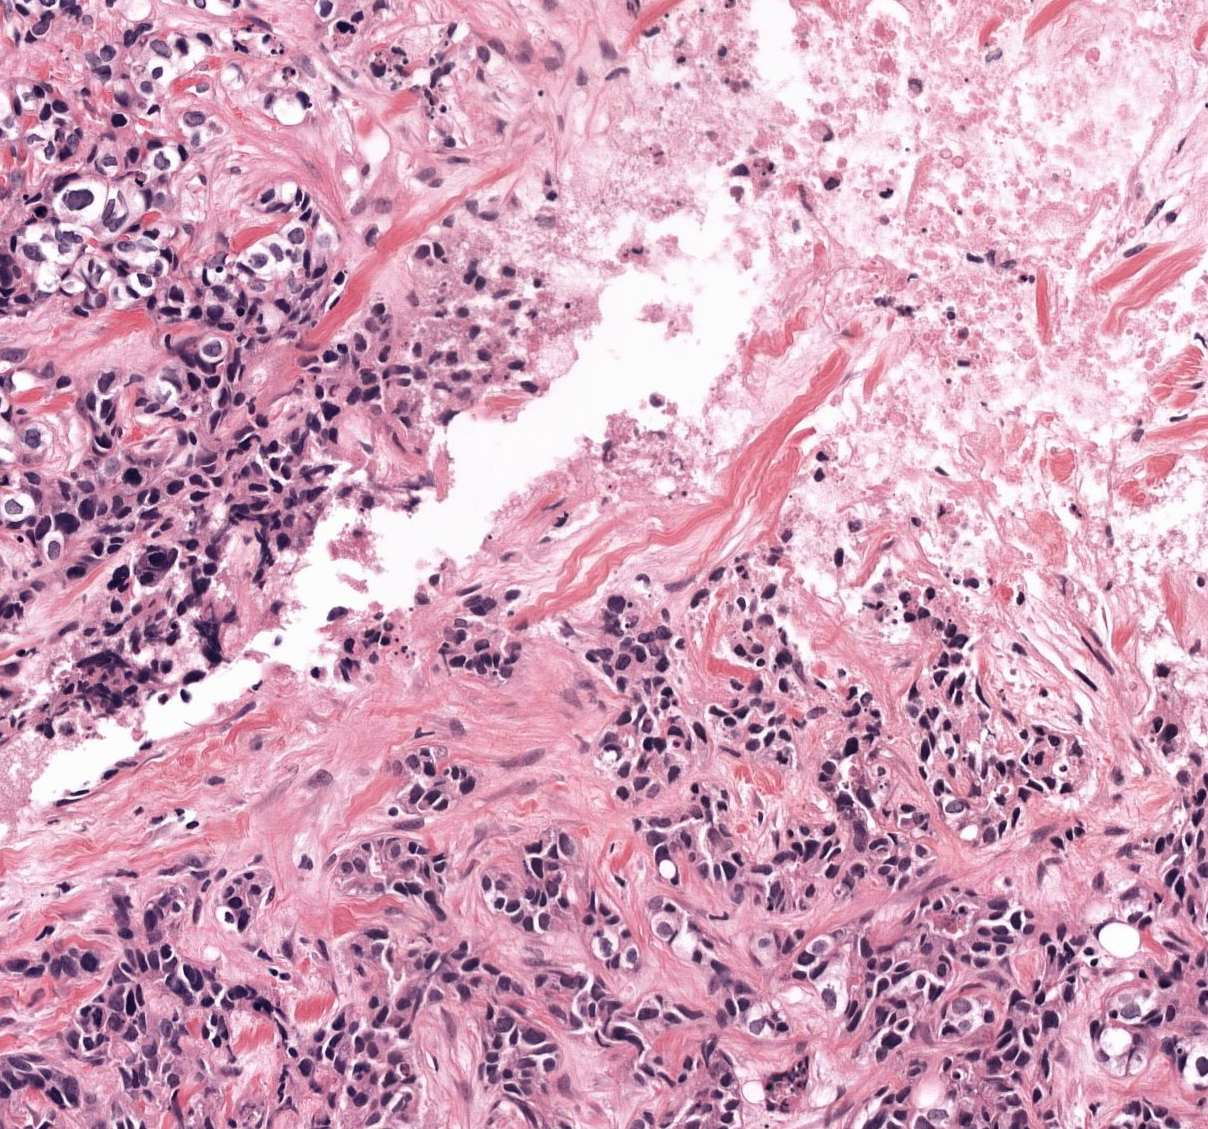
\includegraphics[width=\textwidth]{backdp/tiger_sample.png}
    \caption{TIGER}
    \label{sfig:backdp:challenge_sample:tiger}
  \end{subfigure}
  \begin{subfigure}{0.30\textwidth}
    \centering
    % Lizard_Image1/consep_1.png
    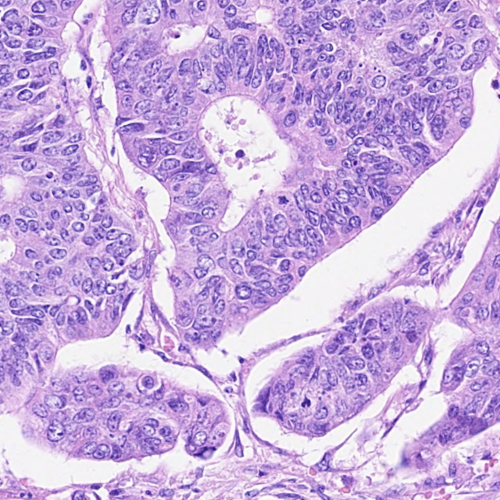
\includegraphics[width=\textwidth]{backdp/lizard_sample.png}
    \caption{CoNiC (Lizard dataset)}
    \label{sfig:backdp:challenge_sample:conic}
  \end{subfigure} 
  \begin{subfigure}{0.30\textwidth}
    \centering
    % 200.tiff
    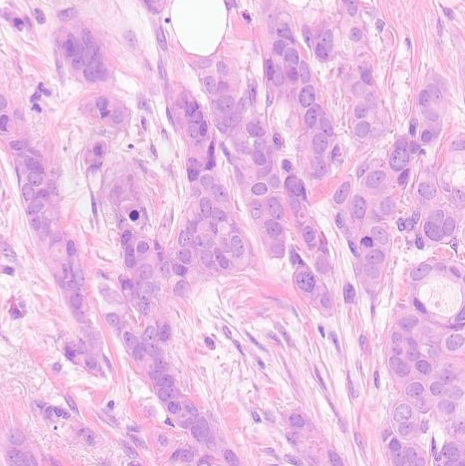
\includegraphics[width=\textwidth]{backdp/midog_sample.png}
    \caption{MIDOG 2021}
    \label{sfig:backdp:challenge_sample:midog}
  \end{subfigure}\\

  \begin{subfigure}{0.30\textwidth}
    \centering
    % 1058.jpg
    \includegraphics[width=\textwidth]{backdp/bcnb_sample.png}
    \caption{BCNB}
    \label{sfig:backdp:challenge_sample:bcnb}
  \end{subfigure}
  \begin{subfigure}{0.30\textwidth}
    \centering
    % train -> 436219-7159-50847-[1, 1, 0].png 
    \includegraphics[rotate=90,width=\textwidth]{backdp/wsss4luad_sample.png}
    \caption{WSSS4LUAD}
    \label{sfig:backdp:challenge_sample:wsss4luad}
  \end{subfigure}
  \begin{subfigure}{0.30\textwidth}
    \centering
    % TCGA-A2-A0YM-01Z-00-DX1.A48B4C96-2CC5-464C-98B7-F0F92AE56533.svs
    \includegraphics[width=\textwidth]{backdp/bcss_sample.png}
    \caption{BCSS}
    \label{sfig:backdp:challenge_sample:bcss}
  \end{subfigure} \\

  \begin{subfigure}{0.30\textwidth}
    \centering
    % rgbs_colorNormalized/TCGA-S3-AA10-DX1_xmin43039_ymin23986_MPP-0.2500.png
    \includegraphics[height=0.22\textheight]{backdp/nucls_sample.png}
    \caption{NuCLS}
    \label{sfig:backdp:challenge_sample:nucls}
  \end{subfigure}
  \begin{subfigure}{0.48\textwidth}
    \centering
    % 
    \TODO{???}
    \caption{PAIP 2021}
    \label{sfig:backdp:challenge_sample:paip2021}
  \end{subfigure} 
  \caption{Samples from the Grand Challenge datasets of our mini-review.}
  \label{fig:backp:samples_challenges}
\end{figure}

In order to illustrate this point, we performed a search on the Grand Challenge website \parencite{grandchallenge}, a popular platform which runs \acrlong{ml} challenges related to biomedical images, each challenge coming with an open-access dataset. We searched for \textit{histology} challenges published in 2021 and found 8 results (see Table \ref{tab:backdp:datascarcity-grandchallenge} for a brief description of relevant aspects and Figure \ref{fig:backp:samples_challenges} for selected samples of these datasets).

A first observation is that, whether the dataset is a set of \acrshort{wsi} or \textit{\acrlong{roi}s} (\acrshort{roi}), the number of provided images is several orders of magnitude below the number of images available in natural image datasets. It can be argued that the dimensions of \acrshort{wsi} and \acrshort{roi} images in \acrlong{dp} datasets is significantly larger that natural images (\eg average image size in ImageNet is 469 $\times$ 387 pixels, the largest of the 151 \acrshort{roi} of BCSS reaches approximately 7k $\times$ 10k pixels), however this must be in perspective in relation to the prediction task. For instance, hundreds of \acrshort{wsi}s represent a very large amount of raw data (\eg few terabytes) but, when the target task is whole-slide classification, this only amounts to a hundreds of annotated samples which is significantly fewer compared to ImageNet or others and can be considered a rather small sample size from a \acrshort{ml} perspective.  

Beyond the size of datasets, it is interesting to note that most prediction tasks in \acrlong{dp} only feature few classes (at most 12 in our Grand Challenge sample). It is common to encounter tasks presented as binary (\eg malignant \vs benign) even though it is often a simplification of the underlying biological or medical problem. Datasets with a large variety of classes have shown to be effective for learning efficient models on natural images. Therefore, on this matter, \acrlong{cpath} is still lagging behind significantly. 

% To the best of our knowledge, there is no single dataset that features more than 100 classes. \TODO{what is the largest?}

It is also interesting to consider how these datasets were built. Among them, four datasets use internal data acquired and annotated specifically for the challenge (PAIP 2021, MIDOG 2021, BCNB, BCSS), two of them mix both internal and external data (TIGER, WSSS4LUAD) and the last two use exclusively data from external sources (CoNiC, NuCLS). Regarding the use of external data, it either means that external \acrshort{wsi} were imported and annotated for the challenge or that data from other datasets were combined together. For instance, the CoNiC challenge is based on the Lizard dataset \parencite{graham2021lizard} which combines data from the \acrfirstit{tcga} \parencite{weinstein2013cancer}, PanNuke \parencite{gamper2019pannuke}, CRAG \parencite{graham2019mild}, CoNSeP \parencite{graham2019hover}, GlaS \parencite{sirinukunwattana2017gland} and DigestPath \parencite{li2019signet}. The \acrshort{tcga} is an open platform gathering various data related to cancer genomic including a little more than 30k \acrlong{wsi}s, making it one of the largest open databases of \acrshort{wsi} to date. It is no surprise that, over the years, many datasets have been built using the \acrshort{tcga} as one of their sources. This also includes WSSS4LUAD, TIGER and NuCLS from our Grand Challenge sample. Interestingly, one of the components of Lizard, PanNuke has also been built from \acrfirst{tcga} and three external datasets of which two were built on top of the same platform (MoNuSeg \parencite{kumar2019multi} and CMP17 \parencite{vu2019methods}). Although it raises the question of the risk of data leakage, assembling existing datasets to form a larger one certainly helps fighting data scarcity.

\subsubsection{Causes}
\label{sssec:backdp:ds-causes}

The mini-review performed in the previous section was not aimed at being a thorough evaluation of \acrshort{dp} datasets characteristics. It rather serves as a way to highlight different consequences of data scarcity in the field: small dataset size, lack of variety and versatility, \etc. The scarcity in \acrlong{dp} is caused by a combination of factors.  

One of the main causes of scarcity is the cost of the annotation process. Pathology is not a simple subject and slide evaluation requires years of training and experience. Whereas classifying pictures into object categories can be done by mostly anyone, creating a ground truth \acrlong{dp} dataset requires trained pathologists for whom time is a precious and expensive resource. Therefore, annotation cost in \acrlong{dp} is significantly higher compared to the natural image domain. This is aggravated by the fact that disagreement between pathologists is not uncommon and quality ground truth usually requires confronting and aggregating annotations by several experts. 


Privacy and ethical concerns also play a role. Indeed, medical data is sensitive and cannot be shared without patient consent, rightfully so, preventing data to be made available for \acrlong{ml}. Privacy might incur additional costs as it might be necessary to keep track where data records have been used, for instance, in the context of the european \acrfirst{gdpr}. Indeed, in case a patient revokes his data sharing agreement, under the right-to-be-forgotten, models might have to be re-trained \parencite{humerick2017taking}. Overall, it can discourage researchers and partictioners to make their data available. 

The use of data-hungry \acrlong{dl} algorithms does not help and is aggravated by the need for a dataset to contain enough samples to account for the variability incurred by the slides content and preparation process. 

% On another front, complexity and duration of the slide preparation process makes it more difficult to produce new \acrshort{wsi} than natural images like pictures which can be captured with any smartphone nowadays. Currently, slide preparation is definitely not a bottleneck as opposed to labeling but could become one if  throughput of quality annotations.

\subsubsection{How to work around data scarcity ?}
\label{sssec:backdp:ds-solutions}

The causes of data scarcity are numerous and it remains a challenge for \acrlong{cpath} but the situation is evolving positively. 

Nowadays, there exist annotation strategies which allow to cut the cost per annotation and therefore produce larger datasets given the same budget. These strategies include crowdsourcing through citizen science \parencite{peplow2016citizen} or the intervention of medical students (\eg NuCLS dataset). These approaches obviously require either supervision by pathologists or more annotations per image to average out the inaccuracies (or even both) but these are in general less expensive than direct annotation by trained pathologists. It is also possible to indirectly reduce the annotation cost by reducing the time spent per annotation. One way of achieving that is to use of \acrshort{ai} to assist experts and accelerate the annotation process (see NuCLS, CoNiC, MIDOG 2021 from our Grand Challenge sample) \parencite{chai2020human}. A weak but fast algorithm could for instance suggest cell boundaries. The annotator could then correct the boundaries if necessary which is less time-consuming then drawing them from scratch. The use of dedicated and intuitive user interface with efficient drawing tools can also help in that regard.  

If annotating new data is not an option, it is also possible to combat data scarcity by the use of existing external data and proper computational methods. There exist several open resources for \acrlong{dp} \parencite{maree2019open} providing access to slides and annotations. We have already introduced \acrshort{tcga} which provides access to a spectacular amount of 30k \acrshort{wsi}. The Camelyon dataset introduced in Section \ref{ssec:backdp:analysis_camelyon} contains 1399 \acrshort{wsi} of which 209 were annotated at full resolution with detailed hand-drawn contours of all metastases. This is one of the largest most-precisely annotated dataset in the field to date. The Lizard dataset (subject of the CoNiC challenge) contains almost 500k segmented nuclei all labelled into one of 6 classes. Some promising projects are also ongoing such as Bigpicture \parencite{moulin2021imi} of which the goals are to ``\textit{create the first European, ethically compliant, and quality-controlled whole slide imaging platform, in which both large-scale data and AI algorithms will exist}''. This project aims at having the same impact on \acrlong{cpath} as ImageNet had on the natural image domain by constructing a database of millions of digital slides.

Sometimes the lack of data is such that the dataset is not representative enough of the different variations that could occur in a realistic context. The impact of this issue can be alleviated during the training process directly with an ad-hoc data augmentation procedure that would automatically generate the kind of variations that can be expected (\eg staining intensity, deformation, \etc.). Data normalization during pre-processing such as stain normalization can also help in that regard \parencite{kang2021stainnet}.

Regarding the computational methods, there exist machine and \acrlong{dl} algorithms which can make use of external or sparse data. We explore some of them in the thesis and present related works in the following sections. 

\subsection{Transfer learning}
\label{ssec:backdp:tl}

Transfer learning (see Sections \ref{ssec:backml:transfer} and \ref{ssec:backml:dl:deeptransfer}) is one of the most popular technique for tackling data scarcity. In this section, we explore how deep transfer learning was applied to biomedical images. Some of the first applications were reported in \parencite{bar2015chest,ciompi2015automatic,van2015off} for pulmonary nodule detection in chest x-rays and \acrshort{ct}-scans using Decaf and OverFeat (feature extractors based on ImageNet and AlexNet) as feature extractors. While those works have revealed the potential of deep transfer learning in that field, the performances were not significantly better than those of previous methods. \citeauthor{ravishankar2016understanding} \cite{ravishankar2016understanding} compared the performance of a pre-trained AlexNet-based CaffeNet \parencite{jia2014caffe} to well-established computer vision like \acrfirstit{hog} \parencite{mcconnell1986method} and found transfer to outperform these features.

Later, as new ImageNet architectures emerged, their transfer potential from ImageNet was also evaluated on various biomedical imaging tasks. \citeauthor{antony2016quantifying} \cite{antony2016quantifying} evaluated the use of fine-tuning and feature extraction of different archictures including VGG16 for quantifying knee osteoarthritis severity on radiographs. \citeauthor{kieffer2017convolutional} \cite{kieffer2017convolutional} compared training from scratch to both feature extraction and fine-tuning for classification and retrieval of pathology images using InceptionV3 and VGG16. \citeauthor{shin2016deep} \cite{shin2016deep} studied the interest of transfer of different architectures including GoogLeNet and AlexNet for thoracoabdominal lymph node detection and interstitial lung disease classification. 

As introduced earlier, some works have shown that transfer learning is likely to provide better performance when the source and target tasks are close \parencite{yosinski2014transferable} or if the source task includes the target domain \parencite{mensink2021factors}. This implies that pre-training models on pathology data directly is a sound approach although it requires a significant amount of source data to make a proper source task. This was confirmed in several contributions.

For instance, \citeauthor{khan2019improving} \cite{khan2019improving} pre-train an InceptionV3 network on a custom dataset generated from Camelyon16 and then transfer the resulting model to a prostate cancer classification task. They show that their pre-trained model outperforms both training from scratch and using an ImageNet pre-trained model. \citeauthor{medela2019few} \cite{medela2019few} also use of transfer learning between two pathology tasks but rather than following a classical supervised pre-training approach, they adopt a self-supervised algorithm by training a siamese network to distinguish between different parts of colorectal tissues. The network is then transferred as a feature extractor on the target task (tumor classification). \citeauthor{shang2019and} \cite{shang2019and} use several datasets (including some unrelated to their target task such as \textit{Dogs vs. cats}) and compare ImageNet and domain-specific pre-training in order to tackle colonoscopy image classification. They also show that pre-training on domain-specific data yield superior performance compared to using ImageNet. \citeauthor{kraus2017automated} \cite{kraus2017automated} train a custom deep neural architecture, DeepLoc, for classifying protein subcellular localization in budding yeast. Then, they assess the transferability of their pre-trained DeepLoc by fine-tuning it on different image sets, including unseen classes, and show that the pre-training is indeed beneficial.

\subsection{Multi-task learning}
\label{ssec:backdp:mtl}

Multi-task learning (see Section \ref{ssec:backml:mtl} and \ref{ssec:backml:dl:deepmultitask}) has been applied to medical imaging. Samala \etal \parencite{samala2017multi} jointly train a classifier on three mammography image datasets (digitized screen-film and digital mammograms) and compare it to single-task training and transfer learning. They show that a multi-task trained network generalizes better than a single-task one. Zhang \etal \parencite{zhang2016deep} use transfer and multi-task learning to derive image features from Drosophila gene expression. MTL has also been applied more specifically to \acrlong{cpath}. Pan \etal \parencite{pan2018multi} apply MTL for breast cancer classification by using a classification loss and a verification loss. The role of the latter is to ensure that features produced by the network differ for images of different classes. Arvaniti \etal \parencite{arvaniti2018coupling} use both weak and strong supervision at once to classify prostate cancer. Shang \etal (mentioned earlier) also evaluate multi-task learning which is the best performing approach on their target task. However, they suggest that more experiments would have to be carried out to assess whether their conclusions are generalizable.

\subsection{Self-training and weakly supervised learning}
\label{ssec:backdp:st}

We have introduced self-training in Sections \ref{ssec:backml:inbetween} and \ref{ssec:backml:dl:selftraining}. It is not surprising that self-training has also been applied to medical image tasks to combat data scarcity \parencite{tajbakhsh2020embracing, peng2021medical} and to \acrlong{cpath} in particular. Most works in this domain currently treat with image classification \parencite{peikari2018cluster, su2019local, koohbanani2021self, jaiswal2019semi, shaw2020teacher} but detection and segmentation have also been explored. \parencite{li2018based} combine weakly-supervised learning and self-training to predict per-pixel Gleason score across entire WSIs. \parencite{li2019signet} build a signet ring cell detector using self-training. To mitigate the impact of erroneous pseudo-label, their approach features a cooperative training step where two models are trained on the pseudo-labels generated by one another during the previous round. Self-training has also been applied to segmentation for other image modalities. To segment cardiac MR images, \parencite{bai2017semi} propose a self-training approach to train a segmentation architecture. In particular, the teacher and student are the same model and the student is not reset between training rounds. Additionally, they apply a \acrfirstit{crf} to refine the model predictions on the unlabeled images. \parencite{fan2020inf} focus on lung infection segmentation in the context of the COVID-19 pandemic. Their approach features a self-training protocol where at every training round, they pseudo-label $K$ new unlabeled images which will be added to the learning set for the next round. 

Semi-supervised literature also concerns the use of imperfect data which relates more to \acrlong{wsl}. This approach has also be explored for biomedical tasks. \parencite{wolny2021sparse} learn from sparse instance segmentation masks using their sparse single object loss which combines an instance-based loss and an embedding consistency loss. They also evaluate their method on two microscopy images datasets. \parencite{bokhorst2018learning} segment tissues from colorectal cancer patients into 13 classes representing different types of tissues. Their dataset is composed of both exhaustively- and sparsely-labeled images. During training, they apply a weight map to tune and balance the contribution of individual pixels to the loss. The masks ignore unannotated pixels.


\section{Wrapping up}

This chapter introduced the domains of digital and \acrlong{cpath} and gave an overview of different challenges encountered in these fields: high variability in the slide preparation and scanning processes, lack of annotated data, high data volumes, etc. These challenges for sure have slowed down the advances in automated image analysis techniques but the situation is evolving quickly as many initiatives are under way to change that. Given the high practical relevance of automated tools in the domain, one can only expect that the interest in \acrlong{cpath} will continue to grow and envision a future where new image acquisition and analysis techniques will not only revolutionize image analysis iteself but also the pathology and diagnosis workflow as a whole. In this thesis, we explore transfer, multi-task and semi-supervised learning in order to tackle \acrlong{cpath} problems and attempt to work around data scarcity.

\part{Transfer learning and digital pathology}
\chapter{Transfer learning from ImageNet}
\label{chap:comp}

%%%%%%%%% ABSTRACT
% \begin{abstract}
% In this paper, 
% \end{abstract}


\begin{overview}{Overview}
    In this chapter, we investigate deep heterogeneous model-based transfer learning as a way to overcome object recognition challenges encountered in the field of \acrlong{dp}. Through several experiments, we explore various uses of pre-trained neural network architectures and different combination schemes with random forests for feature selection. Our experiments on eight classification datasets show that densely connected and residual networks consistently yield best performances across strategies. It also appears that network fine-tuning and using inner layers features are the best performing strategies, with the former yielding slightly superior results. \\

    \textbf{References:} this chapter is an adapted version of the following article 

    \fullcite{mormont2018comparison} \\

    Supplementary materials can be found in Appendix \ref{app:comp}.
\end{overview}

%-------------------------------------------------------------------------------------------------------------------
%-------------------------------------------------------------------------------------------------------------------
%%%%%%%%% BODY TEXT
\section{Introduction}

% In pathology, tissues were traditionally examined under an optical microscope after being sectioned, stained and mounted on a glass slide. During the last years, progress in scanning technologies made possible the high-throughput digitization of glass slides at high resolution. \acrshort{dp} holds promise for biomedical research and clinical routine but raises great challenges for computer vision research \cite{automated-histology-signal-proc-2014}. 
% First and foremost, a laboratory can produce and scan large amounts of slides per day, each of them being a multi-gigapixel image. Moreover, those slides can contain many different kinds of tissues with different staining techniques. Their quantity, variability and size therefore require efficient and versatile computer vision methods. The second challenge is the scarcity of annotated data. Indeed, annotations of digitized slides require expertise and are therefore expensive and tedious to obtain.

% In parallel, \acrshort{dl} has recently had an impressive impact over the computer vision field starting with work of \citeauthor{krizhevsky2012imagenet} \cite{krizhevsky2012imagenet}, which improved previous natural image recognition performances by a large margin. More recently, researchers have been working at applying those new techniques to biomedical imaging \cite{greenspan2016guest,litjens2017survey}. While current results are promising, improvements were not as impressive as they had been for traditional computer vision tasks (recognition of natural scenes or objects such as ImageNet \cite{deng2009imagenet}, face recognition...) which can likely be attributed to the lack of annotated data.

Data scarcity in \acrlong{cpath} is a recurrent problem which can be tackled in several ways, one of them being transfer learning (see Section \ref{ssec:backdp:datascarcity}). In this chapter, we explore how \acrlong{cnn}s pre-trained on ImageNet \cite{deng2009imagenet} (source task) can be transferred to \acrlong{cpath} target tasks as these architectures have shown interesting transfer properties \cite{donahue2014decaf,yosinski2014transferable,sermanet2013overfeat}. At the time of writing the article this chapter is based on (early 2018), the feature extraction and fine-tuning transfer approaches had not been compared thoroughly yet in \acrlong{cpath} and there was no consensus about whether one was better than the other (see related works in Sections \ref{ssec:backml:dl:deeptransfer} and \ref{ssec:backdp:tl}). Moreover, most works involving transfer learning in medical imaging used old architectures such as AlexNet \cite{shin2016deep,bayramoglu2016transfer,antony2016quantifying,ravishankar2016understanding,tajbakhsh2016convolutional,kumar2017comparative,kim2016deep}, GoogLeNet \cite{shin2016deep,bayramoglu2016transfer} or VGG \cite{kieffer2017convolutional,bayramoglu2016transfer,antony2016quantifying,yu2017deep,hou2016automatic,kumar2017comparative}. To the best of our knowledge, only one article used residual networks for transfer learning at that time \cite{yu2017deep} and none were using dense networks.

Therefore, we study thoroughly and compare several strategies that involve feature extraction and fine-tuning. We carry out several experiments over eight object classification histology and cytology datasets. Different combinations of \acrlong{sota} networks and feature selection techniques using random forests are proposed in order to answer questions of high pratical relevance: which network provides best-performing features? How should those features be extracted and then exploited to get the best performance? Is fine-tuning better than using features from off-the-shelf networks? More generally, our empirical study also contributes to confirm the interest of deep transfer learning for tackling the recurrent data scarcity problem in \acrlong{cpath}.

This chapter is organized as follows. We first introduce the eight datasets we have used in Section \ref{sec:comp:datasets}. We present how we implement feature extraction and fine-tuning in Section \ref{sec:comp:methods}. Our experiments and results are presented and discussed in Section \ref{sec:comp:experiments}. We finally conclude in Section \ref{sec:comp:conclusion}. 

\section{Datasets}
\label{sec:comp:datasets}

\begin{table}
    \center 
    \small
    \begin{tabular}{|c|c|c||ccc|c|}
        \hline
        \multirow{2}{*}{Dataset} & \multirow{2}{*}{Domain} & \multirow{2}{*}{Classes} & \multicolumn{4}{c|}{Images} \\
        \cline{4-7}
        & & & Train & Validation & Test & Total \\
        \hline
        CellInclusion (C) & Cyto & 2 & 1644 & 173 & 1821 & 3638 \\ % & 21 & 2 & 22 & 45   % cells_no_aug
        ProliferativePattern (P) & Cyto & 2 & 1179 & 167 & 511 & 1857 \\ % & 19 & 4 & 13 & 36   % patterns_no_aug
        Glomeruli (G) & Histo & 2  & 12157 & 2448 & 14608 & 29213 \\ % & 91 & 12 & 102 & 205   % glomeruli_no_aug
        Necrosis (N) & Histo & 2 & 695 & 96 & 91 & 882 \\ % & 9 & 1 & 3 & 13   % ulg_lbtd2_chimio_necrose
        Breast (B) & Histo & 2 & 14055 & 4206 & 4771 & 23032 \\ % & 22 & 8 & 4 & 34   % ulg_breast
        MouseLba  (M) & Cyto & 8 & 1722 & 716 & 1846 & 4284 \\ % & 9 & 4 & 7 & 20   % ulg_lbtd_lba
        Lung (L) & Histo & 10 & 4881 & 562 & 888 & 6331 \\ % & 669 & 73 & 140 & 882   % ulg_lbtd_tissus
        HumanLba (H) & Cyto & 9 & 4051 & 346 & 1023 & 5420 \\ % & 50 & 5 & 9 & 64   % ulb_anapath_lba
        \hline
    \end{tabular}
    \caption{Sizes and splits of the datasets. The ``Glomeruli'' dataset was first used in \cite{maree2016approach}.}
    \label{tab:comp:dataset_information}
\end{table}

\begin{figure}
    \centering
    \begin{subfigure}[t]{0.225\textwidth}
        \centering
        \includegraphics[width=\textwidth]{comp/illus_necrose.png}
        \caption{Necrosis}
        \label{sfig:comp:dataset:necrosis}
    \end{subfigure}
    \begin{subfigure}[t]{0.225\textwidth}
        \centering
        \includegraphics[width=\textwidth]{comp/illus_patterns.png}
        \caption{ProliferativePattern}
        \label{sfig:comp:dataset:proliferativepattern}
    \end{subfigure}
    \begin{subfigure}[t]{0.225\textwidth}
        \centering
        \includegraphics[width=\textwidth]{comp/illus_cells.png}
        \caption{CellInclusion}
        \label{sfig:comp:dataset:cellinclusion}
    \end{subfigure}
    \begin{subfigure}[t]{0.225\textwidth}
        \centering
        \includegraphics[width=\textwidth]{comp/illus_breast.png}
        \caption{Breast}
        \label{sfig:comp:dataset:breast}
    \end{subfigure} \\
    \begin{subfigure}[t]{0.225\textwidth}
        \centering
        \includegraphics[width=\textwidth]{comp/illus_glomeruli.png}
        \caption{Glomeruli}
        \label{sfig:comp:dataset:glomeruli}
    \end{subfigure}
    \begin{subfigure}[t]{0.225\textwidth}
        \centering
        \includegraphics[width=\textwidth]{comp/illus_lbtd_lba.png}
        \caption{MouseLba}
        \label{sfig:comp:dataset:mouselba}
    \end{subfigure}
    \begin{subfigure}[t]{0.225\textwidth}
        \centering
        \includegraphics[width=\textwidth]{comp/illus_anapath.png}
        \caption{HumanLba}
        \label{sfig:comp:dataset:humanlba}
    \end{subfigure}
    \begin{subfigure}[t]{0.225\textwidth}
        \centering
        \includegraphics[width=\textwidth]{comp/illus_tissus.png}
        \caption{Lung}
        \label{sfig:comp:dataset:lung}
    \end{subfigure}
    \caption{Overview of our eight classification datasets (the display size does not reflect actual image size). For binary classification datasets, negative and positive samples were respectively placed at the top and bottom of the figures.}
    \label{fig:comp:dataset_samples}
\end{figure}
 

Our experimental study uses datasets collected over the years by biomedical researchers and pathologists using the Cytomine \cite{maree2016collaborative} web application. Using this platform, eight image classification datasets were collected which are summarized in Table \ref{tab:comp:dataset_information}. These contain tissues and cells from human or animal organs (thyroid, kidney, breast, lung, \etc.).

For all datasets except Breast, each sample image is the crop of an annotated object extracted from a whole-slide image, a crop being a rectangle image containing exactly the object. The Breast dataset is composed of patches for which the label encodes the type of tissue in which the central pixel is located. Selected image samples for each dataset are shown in Figure \ref{fig:comp:dataset_samples}. 

\section{Methods}
\label{sec:comp:methods}

In this section, we introduce the architectures we have used in Section \ref{ssec:comp:deep_networks}, we describe how we have implemented feature extraction in Section \ref{ssec:comp:feature_extr} and fine-tuning in Section \ref{ssec:comp:meth_fine_tuning}. We also provide details about the training procedure of the final classifier in Section \ref{ssec:comp:final_classifier} and the inference procedure in Section \ref{ssec:comp:prediction}. As discussed in Section \ref{ssec:backml:dl:deeptransfer}, the interest of feature extraction is that it is not as computationally demanding as fine-tuning but, because the transferred model has not been retrained on the target, the features might not be specific enough. Fine-tuning is much more computationally demanding as it implies retraining a usually large model (\ie tens of millions of parameters or more) but make the features more specific and therefore more relevant to the target which usually has a positive effect on performance. 

\subsection{Deep networks}
\label{ssec:comp:deep_networks}

We follow the feature extraction and classification process presented in Figure \ref{fig:comp:diag_feat_extract}, which starts from a deep \acrlong{cnn} $\theta_s$ pre-trained on a source task $\mathcal{D}_s$. In particular, we use ImageNet as the source dataset $\mathcal{D}_s$ and, for each network, the pre-trained weights were retrieved from Keras \cite{chollet2015keras}. For the network $\theta_s$, we evaluate several architectures that have been \acrlong{sota} on the ImageNet classification dataset \cite{deng2009imagenet} or that present interesting trade-off between computational requirements and performances: VGG16, VGG19 \cite{simonyan2014very}, InceptionV3 \cite{szegedy2016rethinking}, ResNet50 \cite{he2016deep}, InceptionResNetV2 \cite{szegedy2017inception}, DenseNet201 \cite{huang2017densely}, and MobileNet \cite{howard2017mobilenets}. In the sequel, those networks will be respectively referred to as VGG16, VGG19, IncV3, ResNet, IncResV2, DenseNet, and Mobile. These networks can be used as feature extractors or fine-tuned, as explained in the following sections.

\subsection{Feature extraction}
\label{ssec:comp:feature_extr}

\begin{figure*}
    \center
    \includegraphics[scale=0.50]{comp/offtheshelf_schema.pdf}
    \caption{Feature extraction from pre-trained convolutional neural networks}
    \label{fig:comp:diag_feat_extract}
\end{figure*}

Images are first resized to match the input dimension of the network. Respectively denoting by $r_I \times c_I \times b$ the height, width, and number of channels of the input image $I$, we extract a square patch $\mathbf{p}$ of (maximum) height and width $min\left(r_I, c_I\right)$ in the center of the image, which is then resized to the network input size $r_p\times c_p\times b$. This extraction process is parameter-free and preserves the aspect ratio of the image, since all pre-trained networks takes square images as inputs (\ie $r_p=c_p$).

The resized patch is then forwarded through $\theta_s$ (loaded with pre-trained weights). Given this input, the output $\mathbf{a}$ of an arbitrary layer $l$ (\ie a set of feature maps) of dimensions $r_a \times c_a \times d$ is extracted where $d$ is the number of feature maps and $r_a$ and $c_a$ are respectively their height and width. Because this tensor can be high-dimensional, one usually applies a dimensionality reduction procedure (\eg global average pooling, principal component analysis, \etc.) to reduce it to $f$ features, yielding a feature vector $\mathbf{z} \in \mathbb{R}^f$.  Here, we limit our analysis to global average pooling (\ie feature maps averaging), which, unlike principal component analysis for example, has the advantage of being parameter-free.

\subsection{Fine-tuned feature extraction}
\label{ssec:comp:meth_fine_tuning}

For our experiments on network fine-tuning, we replace the final fully-connected layer by a fully-connected layer with as many neurons as there are classes in the current dataset. This newly-appended layer being randomly initialized, it is not correlated at all with the transferred network $\theta_s$ yet. In general, it is a good idea to freeze $\theta_s$ and to train this new layer for a few epochs to correlate them. In our case, we perform this ``warm-up'' phase for 5 epochs with a learning rate of $10^{-2}$. Then, we train the whole network for 45 epochs with a learning rate of $10^{-5}$. We use the Adam optimizer \cite{kingma2014adam} with parameters $\beta_1$ and $\beta_2$ respectively set to 0.99 and 0.999 and no weight decay as suggested in the original paper. We use the categorical cross-entropy as a loss function. Fine-tuning is performed using the training set exclusively. Optionally, we use data augmentation to virtually increase the size of the training set. First, a maximum square crop is taken at a random position in the input image. %% (unlike the extraction procedure presented in Section \ref{ssec:comp:meth_general_framework} which took the crop at the center of the image)
Then, random flips and rotations are applied to the resized patches before they are forwarded through the network. The model is evaluated on the validation set and then saved at the end of each epoch. When the fine-tuning is over, we select among the saved models the one that performed the best on the validation set.

\subsection{Final classifier learning}
\label{ssec:comp:final_classifier}
When the features have been extracted for all images of a dataset (either using off-the-shelf or fine-tuned networks), they can be used for training the classifier $h_c$. 
We use either linear \acrshort{svm} \cite{boser1992training} (with a \acrlong{ovr} scheme for multiclass problems), \acrfirst{et} \cite{geurts2006extremely}, or a \acrlong{fc} single layer perceptron, all as implemented in \texttt{scikit-learn} \cite{scikit-learn}. \acrshort{svm} is the most popular classification method when it comes to classifying extracted features. \acrshort{et} are incorporated mainly for their ability to compute feature importance scores. \acrshort{fc} is a natural choice to mimic how the pre-trained network exploits the features. Hyperparameters of all methods were tuned by slide-wise (or patient-wise) $n$-fold \acrlong{cv} on the merged training and validation sets. Namely, they are the penalty $C$ for \acrshort{svm}, the maximum number of features for \acrshort{et}, and the learning rate and number of iterations for the single layer perceptron. Selected values for tuning are given in Appendix Section \ref{app:comp:sec:selectedhyperparameters}.

\subsection{Prediction}
\label{ssec:comp:prediction}
For prediction, the process is similar: patches are extracted from target images, forwarded through $\theta_s$, reduced by global average pooling and classified with the learned classifier $h_c$. As for the fine-tuning, we make additional experiments using directly the fine-tuned network for classifying the images (see Section \ref{ssec:comp:meth_fine_tuning} for parameters).

\section{Experiments}
\label{sec:comp:experiments}

In this section, we propose and thoroughly compare different strategies for extracting and using features from the deep networks introduced previously. We follow a rigourous evaluation protocol described in Section \ref{ssec:comp:protocol}. Strategies are presented and evaluated one after the other in Sections \ref{ssec:comp:exp_last_layer} to \ref{ssec:comp:exp_fine_tuning}, then an overall comparison of strategies is discussed in Section \ref{ssec:comp:exp_comparing}.


\subsection{Performance metrics and baseline}
\label{ssec:comp:protocol}
For performance evaluation, each dataset (presented in Section \ref{sec:comp:datasets}) is randomly splitted into training, validation and test sets. Following the guidelines in \cite{maree2017need}, image patches from the same slide (or patient when this information was available) are all put in the same set to avoid any data leakage (see Section \ref{ssec:backdp:dataleakage}). %Ideally, one should also avoid putting images from the same patient in different sets but this information was not available, except for the Breast data (which was therefore splitted accordingly).  

To evaluate the different transfer strategies, we use two different metrics: the area under the receiving operating curve (ROC AUC) for binary classification problems and the classification accuracy for the multiclass problems. For the sake of readibility, a summary of the scores for all experiments and datasets is given in Table \ref{tab:comp:res_best_scores_per_strategy} whereas the detailed scores are only given in Appendix Section \ref{app:comp:sec:detailed_scores}. In all figures, we plot instead for each method its rank among all methods compared in the same graph averaged over all eight datasets. To associate high rank with best results, we compute the rank when methods are sorted in reverse order of performance (AUC or accuracy). For example, since ten methods are compared in Figure \ref{fig:comp:avg_ranks_last_layer}, the maximum average rank is 22, corresponding to a method being the best one on all eight datasets, and the minimum average rank is 1, corresponding to a method always worse than all others.

As a baseline for comparison, we use the \acrshort{etfl} variant of the tree-based random subwindows classification algorithm presented in Section \ref{ssec:backml:et_image} because it is fast, generic and requires only a slight tuning of the hyperparameters which are either set to their default value or tuned by \acrlong{cv} (see in Appendix Section \ref{app:comp:sec:selectedhyperparameters} for default values and ranges). We do not compare to training from scratch as it has already been shown that transfer learning from ImageNet was generally superior this this approach \cite{shin2016deep, tajbakhsh2016convolutional}.

\subsection{Last layer features}
\label{ssec:comp:exp_last_layer}

\begin{figure}
    \centering
    \includegraphics[width=0.75\textwidth]{comp/last_baseline_bars.png}
    \caption{Average ranks of the methods for the ``\textit{Last layer features}" experiment. Colors encode the choice of classifier for $h_c$ (orange for \acrshort{svm}, green for \acrshort{et} and red for \acrshort{fc}).}
    \label{fig:comp:avg_ranks_last_layer}
\end{figure}

Our first strategy follows the common approach where features are extracted at the last layer of a pre-trained network. In our case, we take the features from the last feature maps before the first fully connected layer (the numbers of extracted features per network are given in Table \ref{tab:comp:n_features_per_net}). For each dataset and network, we then tune and train the three types of classifiers $h_c$ (\acrshort{et}, \acrshort{svm}, and \acrshort{fc}) with the extracted features, on the union of the training and validation sets, and then we evaluate them on the test set. The resulting average ranks for all classifiers and all datasets are given in Figure \ref{fig:comp:avg_ranks_last_layer}.

\begin{table}
    \center 
    \begin{tabular}{|c|c|c|c|}
        \hline
        \multirow{2}{*}{$\mathcal{N}$} & \multicolumn{1}{c|}{\textbf{Last layer}} & \multicolumn{2}{c|}{\textbf{Merged layers}} \\
        \cline{2-4}
        & \# feat. & \# feat. & \# cut \\
        \hline
        Mobile & 1024 & / & /\\ 
        DenseNet & 1920 & 7744 & 9 \\ 
        IncResV2 & 1536 & 17088 & 12 \\ 
        ResNet & 2048 & 15168 & 17 \\ 
%          IncV3 & 2048 & 10112 & 12 \\ 
        IncV3 & 2048 & / & / \\ 
        VGG19 & 512 & / & / \\ 
        VGG16 & 512 & / & / \\  
        \hline
        \textbf{Total} & 9600 & / & / \\
        \hline 
    \end{tabular}
    \caption{Number of features extracted for the ``\textit{Last layer}'' experiment. Total number of features for the ``\textit{Merging features across networks}". Number of features and cut points for the ``\textit{Mering layers features}'' experiment.}
    \label{tab:comp:n_features_per_net}
\end{table}

We observe that \acrshort{svm} and single layer perceptron are more efficient at classifying from deep features than extremely randomized trees, with a slight advantage to \acrshort{svm}. Mobile, DenseNet, IncResV2 and ResNet yield best performances when combined with \acrshort{svm} or single layer perceptron, while for extremely randomized trees, only DenseNet and ResNet are leading the way. Last layer features from VGG16, VGG19 and IncV3 allow most of the time to beat the baseline but they are clearly not competitive with features from the other networks whatever the classifier. Overall, the best performance is obtained by combining ResNet features with \acrshort{svm}.

\subsection{Last layer feature subset selection}
\label{ssec:comp:exp_feat_sel}

\begin{figure}
    \centering
    \includegraphics[width=0.75\textwidth]{comp/rfe_last_et_bars.png}
    \caption{Average ranks for last layers' features classified with \acrshort{et} before (orange) and after (green) selection with \acrlong{rfe}.}
    \label{fig:comp:exp_rfe_last_et_cmp}
\end{figure}

%% While carrying out the ``\textit{Last layer features}'' experiment (see Section \ref{ssec:comp:exp_last_layer}), we have analyzed the feature importances produced by extremely randomized trees. We have noticed that few features of the last layer seemed actually important for predicting the outcome.
Our second strategy aims at checking whether all features extracted from the last layer of the network are important for the final classification or if a small subset of them would be sufficient to obtain optimal performance. To answer this question, we use cross-validated \acrfirstit{rfe} \cite{guyon2002gene} using importance scores derived from extremely randomized trees to rank the features (where the importance of a given feature is computed by adding up the weighted impurity decreases for all tree nodes where the feature is used, averaged over all trees). This method outputs a sequence $\{(S_t,s_t)|t=1,\ldots,T\}$ (built in reverse), where $S_t$ are nested feature subsets of increasing sizes (with $|S_1|=1$ and $|S_T|=k$) and $s_t$ is the \acrlong{cv} performance of an \acrshort{et} model trained on $S_t$. From this sequence, we compute for each dataset:
$$k_{min} = \min_{\{t=1,\ldots,T: s_t\geq \underset{t'}{max} (s_{t'}-l_a)\}} |S_t|,$$
where $l_a$ is a small performance tolerance (set to $0.005$ in our experiment). $k_{min}$ is thus the minimum number of features needed to reach a performance not smaller than the optimal one by more than $l_a$.

On average across datasets and networks, this method selected 7.5 \% of the features (detailed numbers are given in Appendix Tables \ref{app:comp:tab:rfe_selected} and
\ref{app:comp:tab:rfe_selected_prop}). The models re-trained using the selected features yielded comparable performance when using \acrshort{et} as classifier (see Figure \ref{fig:comp:exp_rfe_last_et_cmp}). Feature selection even improved \acrshort{et} performance on the IncV3, VGG19, and VGG16 networks. Using \acrshort{svm} on the selected features however leads to a performance drop compared to \acrshort{svm} with all features (see Appendix Table \ref{app:comp:tab:detailed_first}). We believe that this difference is due to the fact that the selection is optimized for \acrshort{et} and it is thus likely to remove features that are useful for linear \acrshort{svm} and not for \acrshort{et}, which are non-linear approximators.

Our experiments show that, among the available features from the last layer, most of them are uninformative or redundant and therefore only few of them are actually needed for the prediction when using \acrshort{et} as classifier. This conclusion can also be drawn by observing the \acrlong{rfe} \acrlong{cv} curves (see Appendix Figures \ref{app:comp:fig:rfe_1} and 
\ref{app:comp:fig:rfe_2}). For all datasets and networks, the accuracy converges very abruptly to a plateau when the number of selected features increases, which indicates that removing features from the learning set does not impact negatively the predictive power of the models.  

It is also interesting to note that the selected features are not the same across datasets. For instance with DenseNet, for a feature to appear in the subset of best features (determined with the importances obtained during the ``\textit{Last layer features}" experiment) for all datasets, we need to consider a subset of size 1477 (\ie 77\% of the features). We observe similar results for the other networks (see Appendix Table \ref{app:comp:tab:best_subset_size}). On the other hand, there can be a significant overlap between features selected by \acrshort{rfe} for specific pairs of datasets (see Appendix Tables \ref{app:comp:tab:rfe_sub_overlap} and \ref{app:comp:tab:rfe_sub_overlap2}). These results suggest that the best features are task-dependent and that there would be no interest in restricting a priori the subset of transferred features, even when focusing on the domain of \acrlong{cpath}. The fact that we observe a drop of performance when using the best features subset with \acrshort{svm} also suggests that these conclusions cannot be extended to other classifiers without applying \acrshort{rfe} to them as well.
 
 %-------------------------------------------------------------------------------------------------------------------
\subsection{Merging features across networks}
\label{ssec:comp:exp_merge_net}

\begin{figure}
    \centering 
    \includegraphics[height=\textheight]{comp/all_exp_bars.png}
    \caption{Average ranks for all the evaluated methods.}
    \label{fig:comp:res_avg_ranks_all_methods}
\end{figure}

\begin{figure}
    \centering
    \includegraphics[width=0.8\textwidth]{comp/merged_all_merged_perc.png}
    \caption{Average relative importances (across datasets) brought by each studied network when all their last layer features are aggregated. The black bars quantify the proportion of features of each network. The colors indicate the information brought by features of decreasing importances: blue and red features are respectively the most informative and least informative ones. Blue, orange, green and red bars regroup importances of features that respectively and cumulatively bring 10\%, 25\%, 50\% and 100\% of the information for predicting the outcome. For example, the DenseNet bar  reaches approximately $26\%$, meaning that DenseNet features brings about $26\%$ of the information for predicting the outcome. Moreover, the orange and blue segments for DenseNet together reach approximately $10\%$, meaning that, when selecting the subset of most informative features bringing $25\%$ of the information (orange + blue), those of DenseNet bring $10\%$ of information (or $40\%$ of the information of the subset).}
    \label{fig:comp:models_merged_avg_imp}
\end{figure} 

\begin{table}
    \center
    \small
    \begin{tabular}{|l||c|c|c|c|c||c|c|c|}   
      \hline 
      & \multicolumn{8}{c|}{\textbf{Datasets}} \\
      \hline 
      \textbf{Strategy} & \textbf{C} & \textbf{P} & \textbf{G} & \textbf{N} & \textbf{B} & \textbf{M} & \textbf{L} & \textbf{H} \\
      \hline
      Baseline (ET-FL)      & 0.9250 & 0.8268 & 0.9551 & 0.9805	& 0.9345 & 0.7568 & 0.8547 & 0.6960 \\
      Last layer    & 0.9822 & 0.8893 & 0.9938 & \cellcolor{Dandelion}0.9982 & 0.9603 & 0.7996 & 0.9133	& 0.7820 \\
      Feat. select.	& 0.9676	& 0.8861	& 0.9843	& \cellcolor{LimeGreen}0.9994	& 0.9597	& 0.7438	& 0.8941	& 0.7703 \\
      Merg. networks	& \cellcolor{Dandelion}0.9897	& \cellcolor{LimeGreen}0.8984	& 0.9948	& 0.9864	& 0.9549	& \cellcolor{Dandelion}0.8169	& 0.9155	& 0.7928 \\
      Merg. layers	& 0.9808	& 0.8906	& 0.9944	& 0.9964	& 0.9639	& 0.7941	& 0.9268	& 0.7977 \\
      Inner ResNet	& 0.9748	& \cellcolor{Dandelion}0.8959	& 0.9949	& 0.9964	& 0.9664	& 0.8131	& \cellcolor{Dandelion}0.9291	& \cellcolor{Dandelion}0.8113 \\
      Inner DenseNet	& 0.9862	& \cellcolor{LimeGreen}0.8984	& \cellcolor{Dandelion}0.9962	& 0.9917	& 0.9699	& 0.8012	& 0.9268	& 0.7967 \\
      Inner IncResV2	& 0.9873	& 0.8948	& \cellcolor{Dandelion}0.9962	& \cellcolor{Dandelion}0.9982	& \cellcolor{Dandelion}0.9720	& 0.8137	& 0.9234	& 0.7713 \\
%       Inner IncV3		& 0.9836	& 0.8899	& 0.9951	& 0.9964	& 0.9731	& 0.8104	& 0.9201	& 0.7507 \\
       Fine-tuning		& \cellcolor{LimeGreen}0.9926	& 0.8797	& \cellcolor{LimeGreen}0.9977	& 0.9970	& \cellcolor{LimeGreen}0.9873	& \cellcolor{LimeGreen}0.8727	& \cellcolor{LimeGreen}0.9405	& \cellcolor{LimeGreen}0.8641 \\
%%      \hline
%%      \textbf{Best} & 0.9926 & 0.8984 & 0.9977 & 0.9994 & 0.9873 & 0.8727 & 0.9405 & 0.8641 \\
      \hline
      \textbf{Metric} & \multicolumn{5}{c||}{Roc AUC} & \multicolumn{3}{c|}{Accuracy (multi-class)} \\
      \hline
    \end{tabular}
      \caption{Best score for each strategy and each dataset. The best and second best scores are respectively highlighted in green and orange.}
    \label{tab:comp:res_best_scores_per_strategy}
\end{table}

The third strategy consists in merging features from the last layer of all the studied networks. Aggregating all features results in a feature vector of size $9600$. We observe in Table \ref{tab:comp:res_best_scores_per_strategy} and Figure \ref{fig:comp:res_avg_ranks_all_methods} that despite the fact that features from all networks are combined, this strategy gives performance results similar to but not better than using the best single network, both with \acrshort{et} and \acrshort{svm}.

Using forest importance ranking procedure described previously, we further analyze the information brought by the last layer of each network (feature importances averaged across datasets are given in Figure \ref{fig:comp:models_merged_avg_imp}). We observe that the features of DenseNet bring about $26\%$ of information on average while they only account for $20\%$ of all the features. Moreover, the proportion of information brought by the most informative features of DenseNet is higher than for any other network. Following DenseNet, the next most informative networks are IncResV2, ResNet, IncV3 and finally the Mobile, VGG16 and VGG19 networks. 
Surprisingly, the importances brought by the VGG networks relatively to the number of features is non-negligible and higher than the one of ResNet and IncV3. This may indicate that features of those networks are redundant with features of DenseNet and IncResV2 while features of VGG16 and VGG19 are not.


\subsection{Merging features across layers}
\label{ssec:comp:exp_merged_layers}

\begin{figure}
    \centering
    \includegraphics[width=0.75\textwidth]{comp/merged_layers_all_bars.png}
    \caption{Average ranks for models learned on merged layers of networks compared to the baseline.}
    \label{fig:comp:res_avg_ranks_merged_layers}
\end{figure}

This strategy aims at merging features across layers (at several depths) for a given network. Given the results in Section \ref{ssec:comp:exp_last_layer}, we limit our analysis to the IncResV2, ResNet and DenseNet networks. Those three networks have complex structures and many layers which yield plenty of possible cut points for feature extraction. To reduce the number of possibilities, we limit the extraction to bottlenecks of the networks, a bottleneck being a point were several paths are merged into a single one. For ResNet, we have selected the \acrshort{relu} activations of the merging layer after each residual block. For IncResV2, considering all bottlenecks (following an inception-resnet or a reduction block) yields approximately fifty possible cut points, that is more than 100k features. We have decided to subsample those cut points to obtain a number of features closer to those of other networks while covering the network as uniformly as possible along its depth. As far as DenseNet is concerned, we extract features only at the end of dense blocks and after pooling blocks. Indeed, extracting features inside dense blocks would have resulted in duplicated features because of the dense connections.  

In Table \ref{tab:comp:n_features_per_net} are given the information about the generated features vectors for the ``\textit{Last layer}", ``\textit{Merging features across networks}" and ``\textit{Merging layers features}" experiments. Information about the dimensions of the extracted features from inside the networks (before global average pooling) for ResNet, IncResV2 and DenseNet are respectively given in Appendix Tables \ref{app:comp:tab:inner_layers_resnet}, \ref{app:comp:tab:inner_layers_incresv2} and \ref{app:comp:tab:inner_layers_densenet}. The layer names given in those tables are the ones given by the Keras package \cite{chollet2015keras}. 

The average ranks for each layer of all studied networks are given in Figure \ref{fig:comp:res_avg_ranks_merged_layers}. One first observation is that there is no significant difference between \acrshort{svm} and \acrshort{et} in terms of performance, unlike when we use the last layer only. Surprisingly, DenseNet is not performing well with respect to the other network while it was competitive with using the last layer only. Merging the layers actually leads to a drop of performance with respect to using only the last layer for DenseNet, while it leads to a small improvement for the other two networks (see Section \ref{ssec:comp:exp_comparing}).

 
\begin{figure}
    \centering
    \begin{subfigure}[t]{0.8\textwidth}
        \centering
        \includegraphics[width=\textwidth]{comp/dense_net_201_all_merged_perc.png}
        \caption{DenseNet}
    \end{subfigure}\\
    \begin{subfigure}[t]{0.8\textwidth}
        \centering
        \includegraphics[width=\textwidth]{comp/inception_resnet_v2_all_merged_perc.png}
        \caption{IncResV2}
    \end{subfigure}\\
    \begin{subfigure}[t]{0.8\textwidth}
        \centering
        \includegraphics[width=\textwidth]{comp/resnet50_all_merged_perc.png}
        \caption{ResNet}
    \end{subfigure}
%      \subfigure[IncV3]{\includegraphics[width=0.45\textwidth]{images/inception_v3_all_merged_perc.png}}
    \caption{Average relative importances (across datasets) brought by each extracted layer of a network. See Figure \ref{fig:comp:models_merged_avg_imp} for explanation.}
    \label{fig:comp:res_layers_merged_avg_imp}
\end{figure}

As in the previous section, we use feature importances to identify most informative features. Detailed importances plots for each network are given in Figure \ref{fig:comp:res_layers_merged_avg_imp}. These plots clearly show that the most informative features are spread over all layers. We also observe that the relative importance of features in the early layers is higher than the ones in deeper layers. One possible reason is that last layers actually have more features than earlier ones and as shown in Section \ref{ssec:comp:exp_feat_sel}, most of those features are either irrelevant or redundant. Therefore, the extremely randomized trees actually discard most of them them during training. 

Merging features from several layers results in large feature vectors for describing the images. Those large vectors make this method less attractive as it results in longer classifier training time. This is especially true for extremely randomized trees. Unlike in the previous strategy however, feature extraction does not increase computation requirements as only one forward pass through the network is needed to extract all the features.

%-------------------------------------------------------------------------------------------------------------------
\subsection{Inner layers features}
\label{ssec:comp:exp_inner_layers}

\begin{figure}
    \centering
    \includegraphics[width=0.7\textwidth]{comp/all_per_layer_bars.png}
    \caption{Average ranks for the baseline and the models trained using features from layers inside the networks. For each network, the layers are sorted by decreasing depth (from top to bottom).}
    \label{fig:comp:res_avg_ranks_per_layer}
\end{figure}
 
For this strategy, we assess features extracted from each layer separately. The motivation is to determine if there is a layer that, taken alone, yields better performance than the others, and in particular, the last one. We use the same cut points as for the previous experiment (see Section \ref{ssec:comp:exp_merged_layers}), we learn as many \acrshort{svm} classifiers as there are layers, each using the features of a single layer.

Average ranks for each inner layer and each network are given in Figure \ref{fig:comp:res_avg_ranks_per_layer}. In all cases, the last layer features are always outperformed by features taken from an inner layer of the network. The optimal layer is however always located rather at the end of the network, while the first layers are clearly never competitive. Unfortunately, we have not found that a specific layer was better for all datasets, so in practice the choice of the layer should be determined by internal \acrlong{cv} as we did. Interestingly, the baseline either outperforms the early layers of the networks or yield comparable results which tends to indicate that the features provided by ET-FL are somewhat generic, \ie they could be assimilated to features that you would for instance find in the early layers of a classification \acrshort{cnn} (see Section \ref{ssec:backml:dl:deeptransfer}). 

%-------------------------------------------------------------------------------------------------------------------
\subsection{Fine-tuned features}
\label{ssec:comp:exp_fine_tuning}

\begin{figure}
    \centering
    \includegraphics[width=0.8\textwidth]{comp/ft_baseline_bars.png}
    \caption{Average ranks for fine-tuned networks compared to the baseline. Evaluation was done either by using \acrshort{svm} (orange) or \acrlong{et} (green) on the fine-tuned features or by predicting the outcome using the fine-tuned \acrlong{fc} layer directly (red).}
    \label{fig:comp:res_avg_ranks_ft}
\end{figure}

All previous experiments explored strategies using features extracted from off-the-shelf networks. In this last strategy, we investigate fine-tuning as described in Section \ref{ssec:comp:meth_fine_tuning}. We focus on the same three networks as in the previous sections (ResNet, IncResV2 and DenseNet).

The average ranks for the different fine-tuning methods are given in Figure \ref{fig:comp:res_avg_ranks_ft}. With the three networks, best performances are obtained by making predictions directly from the fine-tuned fully connected layer. \acrshort{svm} and \acrshort{et} trained on the features extracted from the fine-tuned networks are clearly inferior, in particular with IncResV2. Note that, for the other two, last layer features extracted from the fine-tuned network are nevertheless better than last layer features from the original network, when used as inputs to \acrshort{svm} (see Figure \ref{fig:comp:res_avg_ranks_all_methods}). Fine-tuning is thus globally improving the quality of the features for these two networks. Overall, the best performance is obtained with fine-tuned DenseNet.


\subsection{Discussion}
\label{ssec:comp:exp_comparing}

To allow comparison of all strategies, the best scores per strategy and dataset are summarized in Table \ref{tab:comp:res_best_scores_per_strategy} and the average ranks of all methods evaluated in the previous experiments are given in Figure \ref{fig:comp:res_avg_ranks_all_methods}.

Concerning the networks, ResNet and DenseNet often yield the best performing models whatever the way they are exploited. They are followed by the IncResV2, Mobile, and IncV3 networks. Performances obtained with the VGG networks are below those of the others.

Regarding the methods, fine-tuning (and predicting with the network) usually outperforms all other methods whatever the network. Especially, this strategy yields significant improvements for the multi-class datasets. For binary datasets, the improvement is often not as impressive, but on three of these datasets, the performances of all methods are already very high (greater than 0.9).

Moreover, for each dataset, there is at least one inner layer that yields the best or second best scores and this best layer is never the last one. This is confirmed by the rank plot (see Figure \ref{fig:comp:res_avg_ranks_per_layer}) that shows that the ranks of the models learned on last layer features are below those using inner layer features. This might be explained by the fact that last layer features are too specific to the source task (\ie natural images).

Merging features across networks and layers yield results similar to using last layer features but they are outperformed by the best inner layers and also by fine-tuning. The inferior performances of these methods could be attributed to the fact that important features are lost among many redundant and/or uninformative ones and they are thus suffering from overfitting. One way to improve these methods could be to perform feature selection. However, given that these methods are already more computationally demanding, they are definitely less interesting than fine-tuning and selecting the best inner layer. In particular, merging features across networks requires a forward-pass through all the selected networks. Although only one pass is needed when merging the layers, it still yields a large feature vector which makes further training and tuning slower, especially for \acrshort{et}.

Throughout the experiments, we have also gained more insights about the extracted features. By performing feature selection, we have discovered that very few features are actually useful for learning efficient \acrshort{et} classifiers on our datasets and the best features are task-dependent. This conclusion might extend to other classifiers as well but it would require additional experiments to prove it.

\section{Conclusion}
\label{sec:comp:conclusion}

We have empirically investigated various deep transfer learning strategies for recognition in \acrlong{cpath}. We have observed that residual and densely connected networks often yielded best performances across the various experiments and datasets. We have also observed that fine-tuning outperformed features from the last layer of off-the-shelf networks. It also appeared that using one network's inner layer features yielded performances slightly superior to using those of the last layer and inferior to fine-tuning but with the advantage of not having to re-train the network. 


\chapter{Multi-task pre-training}
\label{chap:mtask}


\begin{overview}{Overview}
In this work, we investigate multi-task learning as a way of pre-training models for classification tasks in \acrlong{dp}. It is motivated by the fact that many small and medium-size datasets have been released by the community over the years whereas there is no large scale dataset similar to ImageNet in the domain. We first assemble and transform many \acrlong{dp} datasets into a pool of 22 classification tasks and almost 900k images. Then, we propose a simple architecture and training scheme for creating a transferable model and a robust evaluation and selection protocol in order to evaluate our method. Depending on the target task, we show that our models used as feature extractors either improve significantly over ImageNet pre-trained models or provide comparable performance. Fine-tuning improves performance over feature extraction and is able to recover the lack of specificity of ImageNet features, as both pre-training sources yield comparable performance. \\

\textbf{References:} this chapter is an adapted version of the following article

\fullcite{mormont2020multi} \\

Supplementary materials for this chapter can be found in Appendix Chapter \ref{app:mtask}.
\end{overview}

% Note that keywords are not normally used for peerreview papers.
% \begin{IEEEkeywords}
% deep learning, multi-task learning, \acrlong{dp}, \acrlong{tl}
% \end{IEEEkeywords}


% For peer review papers, you can put extra information on the cover
% page as needed:
% \ifCLASSOPTIONpeerreview
% \begin{center} \bfseries EDICS Category: 3-BBND \end{center}
% \fi
%
% For peerreview papers, this IEEEtran command inserts a page break and
% creates the second title. It will be ignored for other modes.


\section{Introduction}

%{\let\thefootnote\relax\footnote{Submitted for review on 30 November 2019. Accepted for publication on 1 May 2020. Romain Mormont, Pierre Geurts and Rapha\"el~Mar\'ee are all affiliated with the Department of Electrical Engineering and Computer Science of the University of Li\`ege, 4000, Li\`ege, Belgium. (e-mail: {\tt r.mormont@uliege.be}, {\tt p.geurts@uliege.be} and {\tt raphael.maree@uliege.be}).}}

In Chapter \ref{chap:comp}, we have investigated \acrlong{tl} using ImageNet \parencite{deng2009imagenet} as a source task and shown that transfer was indeed beneficial for object recognition and classification in \acrlong{cpath}. Although transfer from ImageNet is a valid option, it has also been shown that \acrlong{tl} works best when the target task is similar to the source task \parencite{yosinski2014transferable,mensink2021factors}. Whereas task similarity is hard to define formally, it is clear that the natural image domain (\ie the ImageNet task) is very dissimilar to \acrlong{dp} tasks. Therefore, this question arises: could we get even better performance from \acrlong{tl} by using a \acrlong{dp} pre-trained model instead of an ImageNet one ? Some works \parencite{khan2019improving, medela2019few, kraus2017automated, shang2019and} have advanced that domain-specific pre-training is indeed beneficial but to the best of our knowledge, at the time of writing the article this chapter is based on (early 2020), there was no in-depth study that attempted to answer this question in \acrlong{cpath}. 

A major obstacle preventing this question to be answered is the lack of a large and versatile dataset like ImageNet in \acrlong{dp}. However, the \acrlong{dp} community has made available many small and medium size datasets through challenges and publications over the years. Given its capability to learn from several tasks simultaneously, \acrlong{mtl} is a great candidate to answer our research question and, in this chapter, we investigate \acrshort{mtl} as a way of pre-training neural networks for \acrlong{cpath}. Therefore, this work lies at the crossroad of multi-task and \acrlong{tl} and differs from typical contributions in those fields mostly on the objective. Indeed, we do not use \acrshort{mtl} nor \acrlong{tl} for solving a specific task but rather to pre-train a versatile network to be transferred to new tasks. 

Our main contributions are as follows. \textbf{(1)} We have collected, assembled and transformed heterogeneous \acrlong{dp} datasets into a large versatile pool of classification datasets featuring 22 tasks, 81 classes and almost 900k images (see Section \ref{sec:mtask:data}). \textbf{(2)} We have developed a multi-task architecture and a corresponding training scheme for creating a transferable model from these 22 tasks (see Sections \ref{ssec:mtask:multitask-architecture} to \ref{ssec:mtask:transfer_techniques}). \textbf{(3)} We have developed a robust validation protocol based on a leave-one-task-out scheme for evaluating the transfer performance of our models compared to other approaches (see Sections \ref{ssec:mtask:exp:model_selection} to \ref{ssec:mtask:exp:parameters}). \textbf{(4)} We have evaluated the performance of the resulting multi-task pre-trained models compared to ImageNet ones, both when pre-trained models are used as direct feature extractors and when they are fine-tuned for each target task. We have also compared our approach to a model trained from scratch without any transfer, as well as to a \acrshort{mtl} model trained including the target dataset (see Section \ref{sec:mtask:results}). \textbf{(5)} Our implementation and multi-task pre-trained models are available on GitHub\footnote{\texttt{https://github.com/waliens/multitask-dipath}}. Related works can be found in Sections \ref{ssec:backml:dl:deeptransfer}, \ref{ssec:backdp:tl}, and \ref{ssec:backdp:mtl}.  

\section{Data}
\label{sec:mtask:data}


\begin{table}[t]
    \centering
    \tiny
    \begin{tabular}{|r|c|c|l|c|c|c|c|}
        \hline
        & \textbf{Name} & Type & \multicolumn{1}{c|}{Task} & Organ \& pathology & Stains & Images & Classes \\
        \hline
1 & MITOS-ATYPIA 14 & DET & Detection of mitosis and grading nuclear atypia & breast cancer & H\&E & 64873 & 3 \\
2 & Warwick CRC & DET & Detection and classification of nuclei & colorectal cancer & H\&E & 2500 & 2 \\
3 & Janowczyk1 & SEG & Cell nuclei segmentation & breast cancer & H\&E & 31725 & 2 \\
4 & Janowczyk2 & SEG & Identification of epithelium and stroma & breast cancer & H\&E & 3402 & 2 \\
5 & Janowczyk5 & DET & Detection of mitosis & breast cancer & H\&E & 24870 & 2 \\
6 & Janowczyk6 & CLF & Patch classification for WSI segmentation & breast, invasive ductal carci. & H\&E & 277524 & 2 \\
7 & Janowczyk7 & CLF & Identification of lymphoma subtypes & breast, lymphoma & H\&E & 2244 & 3 \\
8 & Stroma LBP & CLF & Identification of epithelium and stroma & colorectal cancer & IHC & 2313 & 2 \\
9 & TUPAC2016 Mitosis & DET & Detection of mitosis & breast cancer & H\&E & 77853 & 2 \\
10 & BACH18 Micro & CLF & Predominant cancer type classification & breast cancer & H\&E & 4800 & 4 \\ 
11 & Camelyon16 & SEG & Detection of lymph nodes metastases & breast cancer & H\&E & 2922216 & 2 \\
12 & UMCM Colorectal & CLF & Tissue type classification & colorectal cancer & H\&E& 5000 & 8 \\
13 & Necrosis & CLF & Necrosed vs healthy tissue & breast cancer & IHC & 882 & 2 \\
14 & ProliferativePattern & CLF & Prolif. vs non-prolif. classification & thyroid cancer & Diff-Quik & 1857 & 2 \\
15 & CellInclusion & CLF & Cell inclusion vs healthy cell classification & thyroid cancer & Diff-Quik & 3637 & 2 \\
16 & MouseLba & DET & Cell classification in bronchoalveolar lavage & lung cancer & MGG & 4284 & 8 \\
17 & HumanLba & DET & Cell classification in bronchoalveolar lavage & lung cancer & MGG & 5420 & 9 \\
18 & Lung & CLF & Tissue subtype classification & lung & H\&E & 6331 & 10 \\
19 & Breast1 & CLF & Segmentation of cancer tissue & breast cancer & H\&E & 23032 & 2 \\
20 & Breast2 & CLF & Segmentation of cancer tissue & breast cancer & H\&E & 17523 & 2 \\
21 & Glomeruli & CLF & Glomeruli recognition & kidney & M3C & 29213 & 2 \\
22 & Bone marrow & CLF & Cell type classification & bone marrow & H\&E & 1291 & 9 \\
        \hline 
\multicolumn{5}{|c|}{} & \textbf{Total} & 882800 & 81 \\
\hline
    \end{tabular}
    \caption{Datasets that were used for multi-task pre-training. CLF, DET and SEG respectively stand for \textit{classification}, \textit{detection} and \textit{segmentation}. H\&E, IHC and M3C respectively stand for \textit{hematoxylin and eosin}, \textit{immunohistochemistry} and \textit{Masson's trichrome}. \textit{Images} and \textit{Classes} columns give the number of images and classes of the final (possibly transformed) task for this dataset. References: \textbf{(1)} \parencite{roux2014mitos}, \textbf{(2)} \parencite{sirinukunwattana2016locality}, \textbf{(3-7)} \parencite{janowczyk2016deep}, \textbf{(8)} \parencite{linder2012identification}, \textbf{(9)} \parencite{veta2019predicting}, \textbf{(10)} \parencite{aresta2019bach}, \textbf{(11)} \parencite{bejnordi2017diagnostic}, \textbf{(12)} \parencite{kather2016multi}, \textbf{(13-20)} \parencite{mormont2018comparison}, \textbf{(21)} \parencite{maree2016approach} , \textbf{(22)} \parencite{kainz2017training}.} 
    \label{tab:mtask:datasets}
\end{table}

In order to build our pool of tasks, we have collected publicly available datasets (see Table \ref{tab:mtask:datasets}) from as many sources as possible. We have also leveraged the Cytomine \parencite{maree2016collaborative} platform to collect additional datasets annotated by our collaborators. Some publicly available datasets are missing from our pool because either they could not be converted into a relevant classification problem (e.g. KimiaPath24  \parencite{babaie2017classification}, Janowczyk tutorials 3 \& 4 \parencite{janowczyk2016deep}) or we could not actually obtain them from the authors (\eg dead link on download page or datasets not released yet \parencite{gamper2019pannuke}). Most datasets in our pool are H\&E stained images of human breast cancer but some other organs, pathology and stains are represented, as well as cytology samples, and animal tissues. Also missing in the pool is the BreakHis \parencite{spanhol2015dataset} dataset which was kept aside during the development of our multi-task training protocol for final model evaluation and comparison to other transfer approaches published using the dataset (see Supplementary Section E \TODO{supplemental}). 

\begin{figure*}
    \center
    \begin{subfigure}[t]{0.115\textwidth}
        \centering
        \includegraphics[width=\textwidth]{mtask/illus_necrose.png}
        \caption{Necrosis}
    \end{subfigure}
    \begin{subfigure}[t]{0.115\textwidth}
        \centering
        \includegraphics[width=\textwidth]{mtask/illus_patterns.png}
        \caption{ProliferativePattern}
    \end{subfigure}
    \begin{subfigure}[t]{0.115\textwidth}
        \centering
        \includegraphics[width=\textwidth]{mtask/illus_cells.png}
        \caption{CellInclusion}
    \end{subfigure}
    \begin{subfigure}[t]{0.115\textwidth}
        \centering
        \includegraphics[width=\textwidth]{mtask/illus_breast.png}
        \caption{Breast}
    \end{subfigure}
    \begin{subfigure}[t]{0.115\textwidth}
        \centering
        \includegraphics[width=\textwidth]{mtask/illus_glomeruli.png}
        \caption{Glomeruli}
    \end{subfigure}
    \begin{subfigure}[t]{0.115\textwidth}
        \centering
        \includegraphics[width=\textwidth]{mtask/illus_lbtd_lba.png}
        \caption{MouseLba}
    \end{subfigure}
    \begin{subfigure}[t]{0.115\textwidth}
        \centering
        \includegraphics[width=\textwidth]{mtask/illus_anapath.png}
        \caption{HumanLba}
    \end{subfigure}
    \begin{subfigure}[t]{0.115\textwidth}
        \centering
        \includegraphics[width=\textwidth]{mtask/illus_tissus.png}
        \caption{Lung}
    \end{subfigure} \\
    \begin{subfigure}[t]{0.115\textwidth}
        \centering
        \includegraphics[width=\textwidth]{mtask/illus_bonemarrow.png}
        \caption{BoneMarrow}
    \end{subfigure}    
    \begin{subfigure}[t]{0.115\textwidth}
        \centering
        \includegraphics[width=\textwidth]{mtask/illus_camelyon16.png}
        \caption{Camelyon 16}
    \end{subfigure}
    \begin{subfigure}[t]{0.115\textwidth}
        \centering
        \includegraphics[width=\textwidth]{mtask/illus_bach18.png}
        \caption{BACH18 Micro}
    \end{subfigure}
    \begin{subfigure}[t]{0.115\textwidth}
        \centering
        \includegraphics[width=\textwidth]{mtask/illus_janowczyk1.png}
        \caption{Janowczyk1}
    \end{subfigure}
    \begin{subfigure}[t]{0.115\textwidth}
        \centering
        \includegraphics[width=\textwidth]{mtask/illus_janowczyk2.png}
        \caption{Janowczyk2}
    \end{subfigure}
    \begin{subfigure}[t]{0.115\textwidth}
        \centering
        \includegraphics[width=\textwidth]{mtask/illus_janowczyk5.png}
        \caption{Janowczyk5}
    \end{subfigure}
    \begin{subfigure}[t]{0.115\textwidth}
        \centering
        \includegraphics[width=\textwidth]{mtask/illus_janowczyk6.png}
        \caption{Janowczyk6}
    \end{subfigure}
    \begin{subfigure}[t]{0.115\textwidth}
        \centering
        \includegraphics[width=\textwidth]{mtask/illus_janowczyk7.png}
        \caption{Janowczyk7}
    \end{subfigure} \\
    \begin{subfigure}[t]{0.115\textwidth}
        \centering
        \includegraphics[width=\textwidth]{mtask/illus_lbpstroma.png}
        \caption{Stroma LBP}
    \end{subfigure}
    \begin{subfigure}[t]{0.115\textwidth}
        \centering
        \includegraphics[width=\textwidth]{mtask/illus_mitos14.png}
        \caption{MITOS-ATYPIA}
    \end{subfigure}
    \begin{subfigure}[t]{0.115\textwidth}
        \centering
        \includegraphics[width=\textwidth]{mtask/illus_tupac.png}
        \caption{TUPAC2016 Mitosis}
    \end{subfigure}
    \begin{subfigure}[t]{0.115\textwidth}
        \centering
        \includegraphics[width=\textwidth]{mtask/illus_umcm.png}
        \caption{UMCM Colorectal}
    \end{subfigure}
    \begin{subfigure}[t]{0.115\textwidth}
        \centering
        \includegraphics[width=\textwidth]{mtask/illus_warwick.png}
        \caption{Warwick CRC}
    \end{subfigure}
    \caption{Overview of our final classification tasks (the display size does not reflect actual image size). In this figure, we provide only one set of selected samples for Breast1 and Breast2 as their corresponding tasks are similar and they originate both from the same set of WSIs.}
    \label{fig:mtask:dataset_samples}
\end{figure*}

For the collected datasets to be used in a multi-task classification setting, some dataset-specific pre-processing procedures had to be executed on most of them. Applying those procedures, we have constructed a pool of 22 classification tasks which contains both binary and multiclass classification problems. The different pre-processing are detailed in Supplementary Section A \TODO{supplemental}. Whereas we have tried to avoid intra-dataset class imbalance, there is major inter-dataset imbalance regarding the number of images: the smallest dataset contains 882 images whereas the largest one contains almost 300k. However, we believe it is not an issue and can be made of minor significance by adopting an ad-hoc multi-task training protocol (see Section \ref{ssec:mtask:multitask-training}). Selected samples of the final tasks are provided in Figure \ref{fig:mtask:dataset_samples}. 

\section{Methods}
\label{sec:mtask:methods}

\begin{figure}
    \centering
    \includegraphics[width=\textwidth]{mtask/multitask-training.pdf}
    \caption{Multi-task architecture. $\mathcal{L}$ is the multi-task loss (see Section \ref{ssec:mtask:multitask-training}) and $S$ is a softmax layer. $x_j^{(i)}$ and $z_j^{(i)}$ designate respectively the $j^{\text{th}}$ sample of the batch $\mathbf{x}$ and its corresponding features produced by $\theta_s$. This sample belongs to task $t_i$. Features produced for samples of a given task $t_i$ are routed to this task head $\theta_i$. In this example, there is no sample for task 3 in the batch $\mathbf{x}$. Therefore, the corresponding head $\theta_3$ is inactive (\ie produces no output, no parameters update, no gradient computed) for this iteration.}
    \label{fig:mtask:multitask-training}
\end{figure}

In the following section, we present the training and evaluation protocols and the experiments we have carried out. Those experiments have two main objectives. The first is to evaluate how performance of multi-task and ImageNet pre-trained networks compare when transferred to a target task. The second is to better understand how various training hyperparameters and choices impact the transfer of a multi-task pre-trained network. The multi-task architecture and training are described in \ref{ssec:mtask:multitask-architecture} and \ref{ssec:mtask:multitask-training}. We present the different transfer techniques we have used in Section \ref{ssec:mtask:transfer_techniques}. We have developed a model evaluation and selection protocol which is described in Sections \ref{ssec:mtask:exp:transfer_eval} and \ref{ssec:mtask:exp:model_eval} whereas the various parameters we have chosen and/or evaluated as well as the experiments we have carried out are presented in Section \ref{ssec:mtask:exp:parameters}. 

Regarding notations, we consider a multi-task setting with a pool $\mathcal{P}$ of $T$ classification tasks. Each task $\mathcal{D}_i$ has $n_{i}$ training samples and its classification problem features $C_{i}$ classes. $\mathcal{B}$ represents the set containing all samples from a batch and the batch size is denoted by $B = \left|\mathcal{B}\right|$. $\mathcal{B}_{i} \subseteq \mathcal{B}$ is a set that contains all the samples from task $\mathcal{D}_i$ in batch $\mathcal{B}$. 

\subsection{Multi-task architecture}
\label{ssec:mtask:multitask-architecture}

The structure of our multi-task neural network is similar to those of \parencite{shang2019and} and \parencite{strezoski2019many} and is guided by the objective of pre-training a network for transfer. Therefore, we have adopted the architecture presented in Figure \ref{fig:mtask:multitask-training}. The to-be transferred network is shared for all tasks and denoted by $\theta_s$. We attach a head $\theta_i$ to $\theta_s$ for each task $D_i$ in the pool $\mathcal{P}$. The head $\theta_i$ is simply a fully connected layer of dimensions $f_s\times C_{i}$ where $f_s$ is the number of features produced by $\theta_s$. Using such a simple layer has the benefit of making the learning capacity of the heads much lower compared to the shared network (in our experiments $|\theta_s| \gg |\theta_i|, \forall i$), hence forcing $\theta_s$ to learn relevant features for all tasks. In each head, a softmax is attached after the fully connected layer for producing per-task predictions. When forwarding samples in the multi-task network, samples of a given task $D_i$ are only routed through the head $\theta_i$, which outputs predictions for those samples. 

\subsection{Multi-task training}
\label{ssec:mtask:multitask-training}

Classical training choices have to be adapted for the multi-task setting. Regarding batch sampling, we have decided to interleave tasks at the sample level, meaning that a single batch can contain samples from different tasks. Indeed, we believe that if batches containing samples from only a single task were alternated, the network would not see a particular task for $T-1$ iterations, with $T$ the number of tasks, which could make the training harder when $T$ is large.

Given the imbalance in terms of number of images per task, a batch sampling procedure had to be carefully established. Indeed, a simple random sampling across all images would prevent the tasks with fewer images from being seen during training. To overcome this issue, we selected each image in a batch by first randomly sampling a task and then sampling an image from this task, thus giving equal weights to all tasks.

Regarding the training loss, we averaged the categorical cross-entropy over all batch samples taking into account their respective tasks. More precisely, the multi-task loss $\mathcal{L}$ is computed from a batch as:
\begin{equation}\label{eqn:loss}
\mathcal{L} = \frac{1}{B} \sum_{i=1}^T \ell^{(i)}, \ell^{(i)} = - \sum_{j=1}^{\left|\mathcal{B}_{i}\right|} \sum_{k=1}^{C_{i}} y^{(i)}_{j,k} \log \hat{y}^{(i)}_{j,k}
\end{equation}
where $\ell^{(i)}$ is the loss for the batch samples from task $D_i$.

When developing a multi-task algorithm, a crucial question is what should be shared between tasks. By reducing the capacity of the heads of our architecture, we wanted to enforce the training algorithm to find generic features in $\theta_s$ that work well for all tasks. It might be interesting however to provide a way to slightly relax this implicit constraint, with a hyperparameter. To this end, during training, whereas we train the network with a learning rate $\gamma$, we choose to train the heads with a potentially different learning rate given by $\gamma_h = \gamma \times \tau_\gamma$ where $\tau_\gamma \in \mathbb{R}_{\geq0}$ is a multiplicative factor applied to the global learning rate. This new hyperparameter provides a way of tuning the specificity/genericity of the learned shared features.  Indeed, $\tau_\gamma > 1$ makes the heads learning rate larger and gives therefore more flexibility for the heads to adapt, hence relieving the shared network from learning task-specific features. Taking $\tau_\gamma = 1$ results in using the same learning rate for the whole network.

As previously mentioned, each head $\theta_i$ is randomly initialized, whereas we initialize $\theta_s$ with ImageNet pre-trained weights as it has been shown that doing so accelerates convergence in a single-task setting \parencite{mormont2018comparison}. However, it means that trained features of $\theta_s$ are followed directly by the random layers of the heads. This is known to hurt performance in a single-task transfer setting as reported in Yosinski \etal \parencite{yosinski2014transferable} and is aggravated in a multi-task setting. Indeed, during the first training iterations, the heads gradients will be relatively large and will work to turn each head weights from random to relevant with respect to its task. However, the resulting back-propagated gradients in the last layer of $\theta_s$ will be an average of the potentially contradictory signals coming from all the heads. In order to attenuate or eliminate this problem, a simple idea consists in making each head weights relevant to its task before training the whole network by running a warm up phase during which $\theta_s$ is frozen (\ie no weights update, no batch normalization update) and only the heads $\theta_i$ are trained with a learning rate $\gamma_w$. 

While preparing our experiments, we have noticed an issue with batch normalization \parencite{ioffe2015batch} which is a consequence of the \acrlong{tl} settings. Indeed, it has been shown that using a batch normalization-equipped network with datasets across different domains can hurt performance \parencite{li2018adaptive, chang2019domain}. We have applied a simple procedure detailed in Supplementary Section B \TODO{supplemental} in order to correct the problem. Moreover, the fact that samples are routed in different heads during training requires careful treatment of the gradients after the forward phase. This question is discussed in Supplementary Section C \TODO{supplemental}.

\subsection{Transferring a multi-task pre-trained network}
\label{ssec:mtask:transfer_techniques}

We study both deep \acrlong{tl} approaches, namely feature extraction and fine-tuning. In both cases, $\theta_s$ is pre-trained on some source task(s), either ImageNet or several tasks simultaneously in the \acrshort{mtl} setting. For feature extraction, we exclusively use the pre-trained network $\theta_s$ to extract features for all images of the target task. The extracted features can then be used to learn a third-party classifier, a common choice being a linear \acrshort{svm}. For fine-tuning, we further train the shared network $\theta_s$ on the target task by attaching to it a fully connected layer and a softmax. The resulting network is trained using for instance stochastic gradient descent

Both approaches have their own complementary advantages and drawbacks. As mentioned above, feature extraction uses a linear model which is very fast to train and makes it robust to overfitting when working with small target datasets. However, using fixed pre-trained features makes it possible that the features are not entirely suited for the target task (\eg ImageNet vs. \acrlong{dp}), yielding suboptimal performance. Fine-tuning does not suffer from this drawback as the whole network (or a part of it) is retrained on the target task. When using large capacity networks (\eg ResNet or DenseNet), it allows the network to capture and learn task-specific features. This is however an issue when the target dataset is small because the large capacity of the network can lead to overfitting.

\subsection{Evaluating transferability for hyperparameter tuning}
\label{ssec:mtask:exp:transfer_eval}\label{ssec:mtask:exp:model_selection}

Given a set of tasks available to pre-train a \acrshort{mtl} model for future transfer, either by feature extraction or fine-tuning, a question left is how to tune the hyperparameters to train this model. Since we want to optimize the transferability of the model, rather than for example its average performance on the training tasks, we have to design a specific evaluation protocol and a specific metric to assess this transferability for each hyperparameter combination.

For this purpose, we have developed a leave-one-task-out (LOTO) cross-validation scheme, inspired from leave-one-out cross-validation. It consists in removing a set $\mathcal{T} \subset \mathcal{P}$ of one or more tasks from the training pool $\mathcal{P}$, training a multi-task model on $\mathcal{P} \setminus \mathcal{T}$ and then evaluating how the learnt models transfer to the tasks of $\mathcal{T}$. This operation can then be repeated for different $\mathcal{T}$ to increase the stability of the analysis. In our case, we have picked $\mathcal{T}$ to contain only one task when possible. However, it is important that tasks that are closely related are left out together during LOTO cross-validation to avoid data leakage. In our case, there are two pairs of datasets that are subject to this exception. The first is CellInclusion and ProliferativePattern which are different classification tasks coming from the same WSIs. The second is Breast1 and Breast2 which are the same classification tasks generated with different rules from the same expert annotations. Therefore, applying LOTO exhaustively in our settings leads to 20 possible left out sets $\mathcal{T}$. 

The optimal hyperparameter combination might arguably depend on whether the \acrshort{mtl} model will be used for feature extraction or fine-tuning. We have however solely used feature extraction performance as a proxy to evaluate transferability, mainly because we wanted to release a single \acrshort{mtl} model for simplicity, but also to reduce the computational costs of our experiments. More precisely, given a left-out set $\mathcal{T}$ and one of its task $\mathcal{D} \in \mathcal{T}$, we have evaluated transferability of a multi-task pre-trained network trained on $\mathcal{P} \setminus \mathcal{T}$ by using the resulting $\theta_s$ as a feature extractor on $\mathcal{D}$. The training set of $\mathcal{D}$ was used to train the features classifier (\ie a linear \acrshort{svm}, see Section \ref{ssec:mtask:exp:parameters} for details) and the validation set was used to evaluate it. Transfer performance was evaluated by the \acrfirst{acc} for multi-class classification tasks and the area under the receiver operating characteristic curve \rocauc for binary classification tasks. To cope with the randomness induced by heads initialization and mini-batch sampling, each training of a \acrshort{mtl} model was repeated with 5 different random seeds. Note that, at this stage, the test set of $\mathcal{D}$ was kept aside for future comparison of a selected multi-task pre-trained network and comparison to ImageNet transfer (see Section \ref{ssec:mtask:exp:model_eval}).

All the scores resulting from the same hyperparameters combination but different random seeds can be averaged and the resulting average performance can be used to assess transfer performance on a given task $\mathcal{D}$. We need however to aggregate these scores over all (left-out) tasks to assess the overall transferability of a given hyperparameter combination. Averaging ACC and ROC AUC scores over tasks is in general not a good idea as these values depends on the task difficulty and are not directly comparable across tasks. We propose instead to aggregate rankings. More precisely, for each task, the combination of hyperparameters leading to the best model on average was assigned rank $1$ and the worst was assigned the maximum rank. Applying this procedure to all our sets $\mathcal{T}$ produces a rank matrix where $r_{ij}$ is the rank of the $i^{\text{th}}$ combination of hyperparameters evaluated on the left-out task $j$. The best hyperparameter combination is then defined as the one that minimizes the average rank over all left-out tasks:
\begin{equation} \label{eqn:average_ranks}
\overline{r}_i = \dfrac{1}{T_{\text{out}}} \sum^{T_{\text{out}}}_{j = 1} r_{ij}
\end{equation}
where $T_{\text{out}}$ is the number of left-out tasks.

\subsection{Final performance evaluation}
\label{ssec:mtask:exp:model_eval}

Our main objective is to compare transfer from multi-task and ImageNet pre-trained networks. In principle, two nested LOTO cross-validation loops should be adopted to carry out such comparison:  for each left-out task in the external LOTO CV loop, an additional internal LOTO CV loop should be run to find the optimal hyperparameter combination for training the \acrshort{mtl} model to be transferred to the (external) left-out task. Using two nested loops would be however too expensive computationally\footnote{The simplified scheme we present hereafter has already yielded approximately 20k GPU hours of computation. This computation time would have been multiplied by 10 using two nested LOTO CV loops, which was impossible for us to carry out given our available computing resources.}. We have instead adopted the following simplified scheme. A single LOTO cross-validation is run as described in the previous section. Given a left-out task $\mathcal{D}_k$, we select the hyperparameter combination that minimizes the average rank but now excluding task $\mathcal{D}_k$ from the average computation (\ie excluding $r_{ik}$ from the calculation of $\overline{r}_i$ in Equation \ref{eqn:average_ranks}). All the models trained using this hyperparameters combination (\ie one per seed) are transferred to the target task $\mathcal{D}_k$ using both transfer protocols (\ie feature extraction or fine-tuning). The test set of $\mathcal{D}_k$ is used solely to evaluate the resulting transfer performance whereas the training and validation sets can be used by the transfer protocol, feature extraction or fine-tuning, for training and hyperparameter tuning (see Section \ref{ssec:mtask:exp:parameters}).

Unlike with a true double LOTO CV loop, the training and validation sets of the left-out task $\mathcal{D}_k$ are used, in our simplified scheme, to train some of the \acrshort{mtl} models that are transferred to the other tasks for computing the rankings of the hyperparameters combinations for these tasks. However, this is not expected to introduce any bias since the data from task $\mathcal{D}_k$ is neither used to decide on the optimal hyperparameter setting of the \acrshort{mtl} model transferred to $\mathcal{D}_k$ itself (since $r_{ik}$ is excluded from the computation of $\overline{r}_i$), nor to train this \acrshort{mtl} model.

\subsection{Hyperparameters settings and experiments}
\label{ssec:mtask:exp:parameters} 

\begin{table}
    \centering
    \begin{tabular}{|rc|l|c|}
        \hline
        \multicolumn{2}{|c|}{Parameters} & Values & Count \\
        \hline
        Learning rate (LR) & $\gamma$ & $\{10^{-3}, 10^{-4}, 10^{-5}, 10^{-6}\}$ & 4 \\
        LR multiplier & $\tau_\gamma$ & $\{1, 5, 10\}$ & 3 \\
        Shared network & $\theta_s$ & $\{\text{ResNet50}, \text{DenseNet121}\}$ & 2 \\
        Warm up & $w$ & $\{true, false\}$ & 2 \\
        \hline
        \multicolumn{3}{|c|}{Number of combinations $\left|\mathcal{H}\right|$} & 48 \\
        \hline
        \multicolumn{3}{|c|}{with random seeds} & 240 \\
        \hline
    \end{tabular}
    \caption{The multi-task training parameters evaluated using the cross-validation procedure. Using the LOTO scheme, 240 trained models should be transferred to each left out dataset. $\mathcal{H}$ is the set of all hyperparameters combinations.}
    \label{tab:mtask:results:parameters}
\end{table}

The hyperparameters we have studied and their evaluated values are listed in Table \ref{tab:mtask:results:parameters}. Parameters values and training choices were established based on early experiments which evaluated multi-task training stability and convergence. Regarding the selected range of learning rates, values higher than $10^{-3}$ resulted in very unstable or diverging trainings whereas values lower than $10^{-6}$ prevented convergence. As shared network $\theta_s$, we have used two popular architectures ResNet50 \parencite{he2016deep} and DenseNet121 \parencite{huang2017densely}. We have removed the fully connected layer of those networks and replaced it by a global average pooling. Moreover, we have loaded the networks with ImageNet pre-trained weights from PyTorch \parencite{paszke2019pytorch}.

The multi-task network was trained for 50k iterations using batches of size 64 and SGD as optimizer using momentum set to its default value (\ie $0.9$), learning rate $\gamma$ and heads learning rate multiplier $\tau_\gamma$. Either the whole network was trained directly, or the heads were first warmed up for 5k iterations with learning rate $\gamma_w = 10^{-3}$ before the whole network was trained for 45k iterations.

Classical data augmentation and normalization have been applied to the input images. We have used ImageNet statistics for normalizing the images as early experiments have shown no significant improvement by normalizing with per-task statistics. As data augmentation, we have applied simple random vertical and horizontal flips as well as extraction of a random square crop (if the image is not square already).

When feature extraction was applied either during the evaluation or selection, we have used linear \acrshort{svm} \parencite{fan2008liblinear} as feature classifier. Whenever a \acrshort{svm} classifier was trained, we have tuned the $C$ regularization parameter among the following values $\left\{10^{-10}, 10^{-9},...,10^{-1},1\right\}$ by 5-fold cross-validation. The tasks were splitted into folds based on the most relevant information available for the task (patient, slide or image).

Regarding fine-tuning, we have trained the network for 100 epochs on the training set of the target task and have tuned the learning rate among $\{10^{-3}, 10^{-4}, 10^{-5}, 10^{-6}\}$ and have selected the best epoch on the validation set. When transferring from our multi-task pre-trained models, we have performed the selection of the best multi-task models as explained in Section \ref{ssec:mtask:exp:model_selection}. Then, for each model trained with the best hyperparameters (\ie one per seed), we have trained one model per fine-tuning hyperparameters combination. For ImageNet, the approach was slightly different as we had only one model to start from. In this case, we have used 5 different seeds for fine-tuning. 

At this point, it is important to note that LOTO cross validation is quite demanding in terms of computing resources as, for all $\mathcal{T}$, all the combinations of hyperparameters and random seeds have to be evaluated. As indicated in Table \ref{tab:mtask:results:parameters}, 240 models would have to be trained per set $\mathcal{T}$ of excluded tasks which, given 22 tasks, yields 4800 multi-task trainings. Due to limited availability of computing resources, we had to reduce this number and have done so by reducing the number of left out tasks used in our analysis. In particular, we have kept 10 tasks in 8 sets: $\{\text{CellInclusion}, \text{ProliferativePattern}\}$, $\{\text{Breast1}, \text{Breast2}\}$, $\{\text{MouseLba}\}$, $\{\text{HumanLba}\}$, $\{\text{Necrosis}\}$, $\{\text{Lung}\}$, $\{\text{Glomeruli}\}$ and $\{\text{BoneMarrow}\}$ (see Table \ref{tab:mtask:dataset_train_info}). All other tasks were always incorporated however to train each multi-task model.

For the sake of completeness, we have also compared the \acrlong{tl} approaches with training from scratch and joint training. The former consists in training a network initialized with random weights. The latter consists in training a network in multi-task using the whole pool of tasks (including the target tasks). 

For training from scratch, we have used the same settings as for the fine-tuning experiment except for the network weights initialization (using initialization strategy as defined in PyTorch): same evaluated learning rates, number of training epochs and same networks. Regarding joint training, we have used the same architecture and training algorithm as for our multi-task pre-training. For the evaluation tasks listed above, only their training set is used for the multi-task training, while their validation and test sets were respectively used for optimizing the hyperparameters and evaluating the selected model. The data for the other training tasks were kept the same as for multi-task pre-training.

\section{Results and discussion}
\label{sec:mtask:results}
\begin{figure}[t]
    \center
    \begin{subfigure}[t]{0.70\textwidth}
        \centering
        \includegraphics[width=\textwidth]{mtask/dense_fe.png}
        \caption{DenseNet121}
    \end{subfigure}    
    \begin{subfigure}[t]{0.70\textwidth}
        \centering
        \includegraphics[width=\textwidth]{mtask/resnet_fe.png}
        \caption{ResNet50}
    \end{subfigure}    
    \caption{Absolute score difference between multi-task versus ImageNet pre-training using \textbf{feature extraction} as transfer protocol on our ten evaluation tasks. Positive difference indicates that multi-task pre-training yield superior performance. Tasks are sorted by evaluation metric and increasing dataset size. The variability of the multi-task transfer is measured using \textit{two} standard deviations given by the error bars.}  
    \label{fig:mtask:res_featext}
\end{figure}

\begin{figure}[t]
    \centering
    \begin{subfigure}[t]{0.70\textwidth}
        \centering
        \includegraphics[width=\textwidth]{mtask/dense_ft.png}
        \caption{DenseNet121}
    \end{subfigure}    
    \begin{subfigure}[t]{0.70\textwidth}
        \centering
        \includegraphics[width=\textwidth]{mtask/resnet_ft.png}\\
        \caption{ResNet50}
    \end{subfigure}    
    \caption{Absolute score difference between multi-task versus ImageNet pre-training using \textbf{fine-tuning} as transfer protocol on our ten evaluation tasks. See Figure \ref{fig:mtask:res_featext} for details. Error bars are computed using two times the largest standard deviation among the ones resulting from ImageNet and multi-task fine tuning.}  
    \label{fig:mtask:res_finetune}
\end{figure}

\begin{figure}[t]
    \centering
    \includegraphics[width=\textwidth]{mtask/densenet_all.png}
    \caption{Performance comparison of different approaches using DenseNet121: training from scratch (\textit{rand}), feature extraction (\textit{tr-fe}) and fine-tuning (\textit{tr-ft}) using our multi-task pre-trained networks and joint training (\textit{joint}). Each bar is the average performance and its error bar gives twice the standard deviation of a given method over five runs. For exact scores, see Supplementary Table V (\TODO{supplemental}).}  
    \label{fig:mtask:res_all_densenet}
\end{figure}

We report how our methods compare to transfer from ImageNet, training from scratch and joint training in Section \ref{ssec:mtask:transfer_perfromance}. Then, we study the effect on transfer of the various evaluated multi-task training hyperparameters in Section \ref{ssec:mtask:hyperparameters}. Finally, we discuss our results and future works in Section \ref{ssec:mtask:res:discussion}.
%Finally, we evaluate how the best transferable models perform on a held-out dataset in Section \ref{ssec:mtask:breakhis_eval}. 

\subsection{Transfer performance}
\label{ssec:mtask:transfer_perfromance}

\begin{table}[ht]
    \centering
    \begin{tabular}{|c|c|c|c|}
        \hline
        \multirow{2}{*}{\textbf{Task}} & \textbf{Train} & \multirow{2}{*}{\textbf{Full name}} & \multirow{2}{*}{\textbf{Metric}}\\
        & \textbf{size} & & \\  
        \hline
        BoMa & 652 & BoneMarrow & \multirow{4}{*}{\rotatebox[origin=c]{75}{Accuracy}}\\
        MoLb & 2438 & MouseLba & \\
        HuLba & 4397 & HumanLba & \\
        Lung & 5443 & Lung & \\
        \hline
        Nec & 791 & Necrosis & \multirow{6}{*}{\rotatebox[origin=c]{75}{ROC AUC}} \\
        PrPa & 1346 & ProliferativePattern & \\
        CeIn & 1816 & CellInclusion & \\
        Glom & 14605 & Glomeruli & \\
        Br2 & 14953 & Breast1 & \\
        Br1 & 18261 & Breast2 & \\
        \hline
    \end{tabular}
    \caption{Evaluation tasks, their evaluation metric, training set size and full name.}
    \label{tab:mtask:dataset_train_info}
\end{table}


As explained in Section \ref{ssec:mtask:exp:transfer_eval}, we have used both feature extraction and fine-tuning to evaluate transfer performance. We could not repeat our experiments with several datasets splits given the computational cost, which would have allowed us to perform formal statistical tests for method comparison. To ease the discussions below, we will nevertheless call significant any difference between two average errors that exceed, in absolute value, twice the maximum of their standard deviations. If the scores were Gaussian distributed, this would ensure that each average score is outside a 95\%-confidence interval around the other score.


Absolute score differences between feature extraction from ImageNet and multi-task pre-trained networks can be found in Figures \ref{fig:mtask:res_featext}a and \ref{fig:mtask:res_featext}b for DenseNet121 and ResNet50 respectively. Our DenseNet121 features yield superior scores for nine datasets out of ten (all but \textit{Necrose}) of which superiority is significant for all but two (\textit{HumanLba} and \textit{MouseLba}). The score difference is in favor of ImageNet features on \textit{Necrose} although it is not significant. ResNet50 features yield superior results for six out of ten datasets (all but \textit{CellInclusion}, \textit{Glomeruli}, \textit{ProliferativePattern} and \textit{Lung}) of which superiority is significant for all but two datasets (\textit{Necrose} and \textit{Breast1}). Out of the four datasets where ImageNet features yield superior scores, the difference is significant for only one of them (\textit{CellInclusion}). It is interesting to note that the largest difference of scores in favor of ImageNet is only $0.21\%$ (ROC AUC) on \textit{Necrose} for DenseNet121 whereas the difference in favor of our features is at most $3.52\%$ (ACC) on \textit{BoneMarrow}. Similary with ResNet50, the largest differences are $0.91\%$ (ROC AUC) on \textit{CellInclusion} and $6.48\%$ (ACC) on \textit{BoneMarrow} respectively in favor of ImageNet features and ours. Therefore, it appears that the loss of performance when our features underperform compared to ImageNet is lower than the expected gain of performance when our features are better. This indicates that the performance gain or loss you would obtain with multi-task features are dataset dependent and is hard to predict apriori, although the loss of performance is usually small compared to the possible improvement. Another interesting observation is the stability of transfer performance as only four evaluations (out of 20) exhibit standard deviations larger than 0.5\% (ROC AUC or ACC). 

Regarding fine-tuning, our features outperform ImageNet ones for five and six datasets with DenseNet121 and ResNet50 respectively (see Figures \ref{fig:mtask:res_finetune}a and \ref{fig:mtask:res_finetune}b). However, none of the differences are significant whether or not the advantage is in favor of our approach.

As a summary, feature extraction transfer approach seems to benefit from multi-task pre-training as 15 evaluations (out of 20) are in favor of our approach of which 11 are significant. Only two evaluations are significantly in favor of ImageNet features.  However, fine-tuning from our features yield comparable performance with ImageNet features initialization as no score difference is significant (11 evaluations are in favor of our approach).

As an additional experiment, we compare transfer by feature extraction and fine-tuning with a similar model trained from scratch and the joint \acrshort{mtl} approach described in Section \ref{ssec:mtask:exp:parameters} (see Figure \ref{fig:mtask:res_all_densenet}). These experiments show that fine-tuning improves over feature extraction significantly on most datasets and that training from scratch is subpar compared to the transfer approaches, feature extraction included. Both observations confirm previously published results \parencite{ponzio2019dealing, tajbakhsh2016convolutional,shin2016deep} and our conclusions in Chapter \ref{chap:comp}. It appears that joint training significantly improves the performance on small datasets (\textit{BoneMarrow} and \textit{ProliferativePattern}) over all other approaches. For larger datasets, performance seem to lie between fine-tuning and feature extraction, or to be on par with fine-tuning on the datasets where the task is almost solved (ROC AUC or ACC close to 1). 

\subsection{Study of multi-task training hyperparameters}
\label{ssec:mtask:hyperparameters}

\begin{figure}[t]
    \centering
    \includegraphics[width=0.7\textwidth]{mtask/densenet121_ulb_anapath_lba_learning_rate_main.png}
    \caption{Distributions of scores per learning rate on DenseNet121 with HumanLba dataset. Each boxplot results from the aggregation of the transfer scores of all models using the same learning rate value on the given network and dataset.}
    \label{fig:mtask:lr_effect}
\end{figure}

\begin{figure}[t]
    \centering
    \begin{subfigure}[t]{0.70\textwidth}
        \centering
        \includegraphics[width=\textwidth]{mtask/bar_lrhm_1e-4_densenet121_ulb_anapath_lba.png}
        \caption{HumanLba}
    \end{subfigure}    
    \begin{subfigure}[t]{0.70\textwidth}
        \centering
        \includegraphics[width=\textwidth]{mtask/bar_lrhm_1e-4_densenet121_ulg_lbtd_lba.png}
        \caption{MouseLba}
    \end{subfigure}    
    \caption{Transfer performance for combinations of the hyperparameters $\gamma_\tau$ (learning rate heads multiplier, \textit{lrhm}) and $w$ (warm up) on two different datasets with learning rate $\gamma = 10^{-4}$ on DenseNet121. Error bars report twice the standard deviation.}
    \label{fig:mtask:hyper_other_effect}
\end{figure}

Our experiments have shown that the hyperparameter impacting transfer performance the most was the multi-task training learning rate. Figure \ref{fig:mtask:lr_effect} shows the distributions of scores per learning rate using DenseNet121 and \textit{HumanLba} dataset. We have picked this plot specifically because it exhibits the most frequent pattern regarding the effect of the learning rate. Similar plots for other datasets as well as ResNet50 can be found in Section D \TODO{supplemental} in the Supplementary Materials. We have observed that the highest learning rate $10^{-3}$ yielded highly variable performance where were most of the time inferior compared to lower learning rates. It indicates that this specific value is too high to cope with the multi-task setting as it prevents the models from making use of the tasks information efficiently. This is likely due to training instabilities (convergence issues, noisy training loss) and overfitting. It appears that the lowest learning rate $10^{-6}$, although yielding more stable performance, generally underperforms higher learning rates $10^{-5}$ and $10^{-4}$. For both networks and most datasets, the latter learning rate $10^{-4}$ is the best performing on average.

The impact of the two other hyperparameters $\tau_\gamma$ and $w$ seems to be minor for most datasets as variation stays within two standard deviations. Moreover, there is no pattern emerging from our experiments regarding those hyperparameters in general. Two exceptions to this observation are the \textit{HumanLba} and \textit{MouseLba} datasets which exhibit significant performance variations on both networks. The variations are shown in Figure \ref{fig:mtask:hyper_other_effect} (similar figures can be found for other networks and datasets in Supplementary Section D). Those Figures show that \textit{HumanLba} benefits from warming up whereas \textit{MouseLba} performance are hurt. This indicates that the effect on transfer performance of warming up and multiplying heads learning rate is very dataset dependent and no general rule can be drawn from our experiments.

\subsection{Discussion and future works}
\label{ssec:mtask:res:discussion}


Features extracted from our models are in general superior to ImageNet ones %(see feature extraction results in Section \ref{ssec:mtask:transfer_perfromance})
which shows that multi-task pre-training is effective at creating task-specific features. This important observation confirms the conclusions of previous works that domain-specific pre-training is a good idea and also validates the multi-task approach when a large source dataset is not available. 

The second important observation is that fine-tuning does not benefit from using our models as we obtain similar transfer performance whatever the source. This indicates that fine-tuning is able to recover the lack of specificity of ImageNet features compared to ours. It contradicts our initial hypothesis that transfer should work better when source and target domains are similar. There might be several reasons why we observe such phenomenon. First, Yosinski \etal \parencite{yosinski2014transferable}, who concluded about the importance of task similarity for efficient transfer, performed their experiments on simple architectures (\eg simple stack of convolutional layers). In our case, we have used more recent architectures (\ie residual and densely connected networks) which are easier to train and might be less impacted by their initial weights. Second, most previous works have shown that fine-tuning was beneficial in a single source task transfer scenario exclusively. Our multi-task pre-training is able to learn specific features but we can not exclude that a more advanced approach could result in even stronger features and might change our conclusion that fine-tuning does not benefit from \acrshort{mtl} transfer. For instance, some papers have highlighted training difficulties associated with multi-task (\eg gradients interference \parencite{yu2020gradient}) and \acrlong{tl} (\eg batch normalization \parencite{chang2019domain}) that could be investigated in our context. In addition, it is likely that, given a target task, not all tasks in the pool contribute equally to transfer performance. A negative transfer phenomenon might even be at play and some tasks might have a destructive effect during the pre-training phase (\ie if they were removed, transfer performance would increase). Incorporating a training mechanism that could dynamically increase (\textit{resp.} decrease) the contribution of constructive (\textit{resp.} destructive) tasks would certainly help improving the resulting features. Alternatively, instead of using all the tasks, one could find a mechanism for selecting a subset of (the most relevant) source tasks for a given target task. Such solution would entail however a significant additional computational cost, since a new \acrshort{mtl} model would have to be trained for each new target task.

There are also several interesting research directions regarding the architecture. On the one hand, it would be interesting to study the effect of increasing the capacity of the task-specific parts. On the other hand, we have only worked with classification tasks so far but it is possible to incorporate directly segmentation or detection tasks to the pre-training by appending an ad-hoc network as a head. Hopefully, enriching the training signal with a dense prediction task such as segmentation could improve the transferability of the resulting models. However, this approach also raises pratical questions and issues such as model memory usage or loss aggregation. 

\section{Conclusion}

In this work, we have investigated the use of multi-task learning for pre-training neural networks in \acrlong{dp}. We have first created a pool of classification tasks from existing sources containing almost 900k \acrlong{dp} images. Using this pool, we have pre-trained a neural network in a multi-task setting in order to transfer the resulting model to unseen \acrlong{dp} tasks. Using a robust evaluation protocol, we have shown that transferring a model pre-trained in multi-task can be beneficial for the performance on the target task. When compared to transfer from ImageNet, our pre-training approach coupled with feature extraction yields comparable or better performance depending on the target dataset. We have observed that fine-tuning multi-task or ImageNet pre-trained models yields comparable performance. It suggests that fine-tuning is able to recover from the lack of feature specificity whatever the pre-training source. However, pre-training remains crucial, as models trained from scratch are clearly inferior. 


\part{Image segmentation}
\chapter{Self-distillation}
\label{chap:sdist}


\lipsum[1-13]
\chapter{Biaflows}
\label{chap:biaflows}

\lipsum[1-13]

% ========== %
% BACKMATTER %
% ========== %
\backmatter

\appendix
\chapter{Appenbix}

\newpage

\listoffigures
\listoftables

\printbibliography

\end{document}
